%
% TU/e Style Master Thesis template for LaTeX
%
% Public version 1.0
% 2010 - 2013 Thijs Nugteren and Joos Buijs
%
% THIS IS THE MAIN FILE (i.e. compile this file, compiling the others directly won't work)
%
\documentclass[a4paper,10pt,twoside]{report}

%all the other includes etc. are done in the thesis.sty file.
\usepackage{thesis}
\usepackage{amssymb}
\usepackage{nomencl}
\usepackage{hyperref}
\usepackage{apacite}
\usepackage{enumitem}
\usepackage{multirow}
\makenomenclature
\newcommand{\nomunit}[1]{\renewcommand{\nomentryend}{\hspace*{\fill}#1}}
\usepackage{etoolbox}
\renewcommand\nomgroup[1]{%
	\item[\bfseries
	\ifstrequal{#1}{S}{Symbols}{%
		\ifstrequal{#1}{G}{Greek symbols}{%
			\ifstrequal{#1}{Z}{Subscripts}{}}{%
			\ifstrequal{#1}{A}{Abbrevations}{}}}%
	]}
\usepackage{tabularx}
\usepackage{listings}
\usepackage{color}

\definecolor{codegreen}{rgb}{0,0.6,0}
\definecolor{codegray}{rgb}{0.5,0.5,0.5}
\definecolor{codepurple}{rgb}{0.58,0,0.82}
\definecolor{backcolour}{rgb}{0.95,0.95,0.92}

\lstdefinestyle{mystyle}{
	backgroundcolor=\color{backcolour},   
	commentstyle=\color{codegreen},
	keywordstyle=\color{magenta},
	numberstyle=\tiny\color{codegray},
	stringstyle=\color{codepurple},
	basicstyle=\footnotesize,
	breakatwhitespace=false,         
	breaklines=true,                 
	captionpos=b,                    
	keepspaces=true,                 
	numbers=left,                    
	numbersep=5pt,                  
	showspaces=false,                
	showstringspaces=false,
	showtabs=false,                  
	tabsize=2
}

\lstset{style=mystyle}
\setlength{\tabcolsep}{12 pt}
\renewcommand{\arraystretch}{2}
\usepackage{adjustbox}
\usepackage{lipsum}
% These commands need to be defined in order to produce a correct and personalized document
%
\newcommand{\shortdoctitle}{Master's Thesis}
\newcommand{\doctitle}{Ultra-wide Band for Vehicle Platooning }
\newcommand{\docsubtitle}{Master Thesis}

\newcommand{\me}{Abhishek Srujan \\ Student Id: 0977110 \\ Email: a.srujan@student.tue.nl}
\newcommand{\keywords}{keyword1, keyword2, keyword3}
\newcommand{\version}{}
\newcommand{\monthYear}{July 2016}

%Be sure to use all the titles for your committee members!!! (their names show up on the very first page!)
\author{\me}

%
% PDF settings
%
\hypersetup
{
    pdfauthor={\me},
    pdftitle={\shortdoctitle},
    pdfsubject={\doctitle},
    pdfkeywords={\keywords}
}

\begin{document}

%use this include for PDF and distribution versions
\pagenumbering{roman}
\begin{titlepage}
	\begin{center}
		
		
		
\includegraphics[width=6cm,,height=1.5cm]{figures/logotue}
		\hspace*{3cm}~%
		
\includegraphics[width=4cm,,height=1.5cm]{figures/logonxp} \\[2cm]
		\large
		\begin{center}
			Department of Mathematics and Computer Science  \\
			EIT ICT Masters Embedded Systems
		\end{center}
		\vspace*{10cm}
		\setlength{\TPHorizModule}{1mm}
		\setlength{\TPVertModule}{\TPHorizModule}
		% Set the Paragraph Indent to zero, so the first line is not Indented
		% Back-up the current value so it can be put back at the end of the title page
		\newlength{\backupparindent}
		\setlength{\backupparindent}{\parindent}
		\setlength{\parindent}{0mm}			
		% Begins a textbox at 72 mm from the left of the edge of the paper and 89 mm from the top
		% The width of the textbox is 95 mm (167 - 72 mm)
		% The height of the box cannot be defined, so it is your task to keep the text not too long
		
		\begin{textblock}{120}(52,89)
			\vspace*{10mm}    
			\noindent\makebox[\linewidth]{\rule{\textwidth}{1pt}}
			\huge
			\textbf{\doctitle \\}
			\huge
			\noindent\makebox[\linewidth]{\rule{\textwidth}{1.2pt}}    
			\Large
			\vspace*{6mm}
			\textit{\docsubtitle}\\
			\vspace*{10mm}
			\Large
			\me\\
		\end{textblock}
		
		

\begin{table}[h]
	\centering
	\resizebox{\textwidth}{!}{%
		\begin{tabular}{ll}
			\textbf{First Supervisor NXP}        & dr. Gerardo Daalderop     \\
			\textbf{Second Supervisor NXP}        & dr. ir. Bart Vermeulen    \\
			\textbf{Supervisor University} & dr. Majid Nabi Najafabadi
		\end{tabular}%
	}
\end{table}


%\vfill
%\vspace*{1cm}
%\Large
%\version

\vfill
%\docdate \\
%\LARGE
%Eindhoven University of Technology \\
\Large 
\vspace*{1cm}
\Large
Eindhoven, August 2016\

% Put the Paragraph Indent back to its original value
\setlength{\parindent}{\backupparindent}
\end{center}
\end{titlepage} 

\normalsize

\clearemptydoublepage

%Sometimes line numbers are nice, uncomment the next line to enable:
%\linenumbers

%It could be handy to have a list of todos and brainstorms in your thesis
%\chapter*{*General todos*}\todo{remove this chapter}
%\input{chapters/general_todos}

%\chapter*{*Brainstorm results*}\todo{remove this chapter}
%\input{chapters/brainstorm_results}


\chapter*{Abstract}\label{chapter:abstract}
Highly Automated Driving is experiencing a huge interest worldwide from many stakeholders. It holds the promise of increasing safety, comfort, personal productivity or entertainment, traffic efficiency, cost and environmental benefits. One area of investigation is the ability of cars to drive closer together, or even to platoon. Since physical sensors such as radars and cameras do not provide the required system performance, reliable communication between vehicles is a means to achieve this. While the wireless communication standard ITS-G5 is being selected as the technology of choice, ultra - wideband (UWB) as a second independent communication technology may provide additional benefits. UWB physical layer enables accurate ranging at low latency, improved robustness against interference, ultra low power consumption, low power spectral density, low cost, low impact on existing narrowband systems and lower probability of intercept and detection.

In this thesis, we investigate the feasibility of using UWB next to WiFi-p, examine the robustness of UWB communication in platooning mode with respect to differences in velocities, typical inter-vehicle environment, outdoor environment and ascertain the ranging accuracy that can be achieved through UWB. We implemented a test platform, TP-UWB (Test Platform for evaluation and analysis of UWB) using LPCXpresso 4337 and DecaWave DW1000 UWB transceiver. The test platform enables us to measure the UWB link quality and range, perform test automation by varying test parameters that influence UWB behavior such as packets or message, channels, Pulse Repetition Frequency (PRF), preamble lengths, preamble codes, standard or non-standard Start of the Frame Delimiter (SFD) and Smart Power enablement. We conduct experiments in table-top, outdoor and inter-vehicle environments using the test platform. We then perform a behavioral analysis of UWB using different parameters indicated above and determine the best configuration of UWB for platooning such that it operates with least possible interference to WiFi-p.

Conclusion not included for reasons of confidentiality.

\textbf{Keywords}: Platooning, UWB, WiFi -p, Interference, Range, Ranging.  

\clearemptydoublepage
\chapter*{Acknowledgments}\label{chapter:acknowledgment}
The last 6 months in NXP Semiconductors was truly an amazing experience. The project was challenging and intriguing at the same time. I would like to take this opportunity to thank few people (to keep it short) who helped me during this project period. My supervisors at NXP, Gerardo Daalderop, and Bart Vermeulen helped me stay motivated and right-on-track all the time with their enthusiasm and dynamic decisions. My supervisor at the University, Majid Nabi Najafabadi, with his guidance, periodic instructions and advice helped me fulfill all the academic requirements to complete this project successfully. I would like to express my gratitude to Joost van Doorn who helped me in critical situations. I would also like to thank Lars van Meurs, Han Raajimakers, Oswald Moonen and Stefan Drude who helped me understand challenging topics. 

I also extend my thanks to my friends Josep Stalin Maria Jebamalai, Sai Janani Ramachandran, Anand Bhaskaran Chethan Shettar, Mridul Krishna and Shivaram Singh Rajput who are my constant pillars of support at all times and helped me stay positive and inspired.

I would like to thank my parents and my family for supporting me and encouraging me to pursue my Master's studies in Europe.  

I would also like to thank EIT ICT Labs for providing me with this great opportunity to be a part of two top-notch European Universities (Technical University of Berlin, Germany and Technical University of Eindhoven, Netherlands). Their continuous support and guidance during the past two years were invaluable.
\clearemptydoublepage
%An executive summary if you want:
%\chapter*{Executive summary}\label{chapter:executive_summary}
%\input{chapters/executive_summary}

%\clearemptydoublepage


%\chapter*{Preface}\label{chapter:preface}
%\input{chapters/preface}

%\clearemptydoublepage

\tableofcontents

%\clearemptydoublepage

\listoffigures

%\clearemptydoublepage

\listoftables
%\newpage
\addcontentsline{toc}{chapter}{Nomenclature}
\renewcommand{\nomname}{Nomenclature}
\markboth{NOMENCLATURE}{NOMENCLATURE}
\printnomenclature

%\clearemptydoublepage
%\printnomenclature

\lstlistoflistings

\clearemptydoublepage
\chapter{Introduction}\label{chapter:introduction}
\setcounter{page}{0}
\pagenumbering{arabic}
%%from here on, start the 'real' page numbering, from 1, with normal digits
\nomenclature[A]{UWB}{Ultra-Wide Band}
\nomenclature[A]{TP-UWB}{Test Platform for evaluation and analysis of UWB}
\nomenclature[A]{PRF}{Pulse Repetition Frequency}
\nomenclature[A]{SFD}{Start of the frame Delimiter}
\nomenclature[A]{ADAS}{Advanced Driver Assistance Systems}
\nomenclature[A]{ESP}{Electronic Stabilization Program}
\nomenclature[A]{ABS}{Anti-lock Braking System}
\nomenclature[A]{CACC}{Cooperative-Adaptive Cruise Control}
\nomenclature[A]{V2V}{Vehicle to Vehicle Communication}
\nomenclature[A]{PER}{Packet Error Ratio}
\nomenclature[A]{ITS}{Intelligent Transport System}
\nomenclature[A]{IVC}{Inter Vehicle Communication}

\section{Context}
Automated Driving is seen as one of the key innovation areas shaping our future mobility and quality of life. The main drivers for higher levels of automated driving are the following:
\begin{itemize}
	\item Safety: Reduce accidents caused by human errors.
	\item Efficiency and environmental objectives: Increase transport system efficiency and reduce time in congested traffic. Smoother traffic will help to decrease the energy consumption and emissions of the vehicles.
	\item Comfort: Enable user's freedom for other activities when automated systems are active.
	\item Social inclusion: Ensure mobility for all, including elderly and impaired users.
	\item Accessibility: Facilitate access to city centers.
\end{itemize}
In technology terms, the advancement towards highly automated driving is seen as an evolutionary process to ensure that all involved stakeholders can develop and evolve with adequate pace. This process already started with the development of Advanced Driver Assistance Systems (ADAS)  like Anti-lock Braking System (ABS) and Electronic Stabilization Program (ESP), and will progressively apply to more functions and environments.

For the domain of commercial vehicles, especially trucks, platooning (based on Cooperative- Adaptive Cruise Control, i.e., C-ACC) is regarded as one of the most promising applications based on automated driving technologies, that improve safety (reduction of human error), efficiency (approx. 10\% fuel reduction, transport or labor efficiency), and comfort for the driver. Platooning implies that the platoon is led by a vehicle which is driven by a professional driver. This driver must have a valid license and is assumed to have additional training for leading a platoon. The following vehicles are under automated longitudinal and lateral control. The following vehicle driver must be able to take over control of the vehicle in the event of a controlled or unforeseen dissolving of the platoon. Following are the advantages of platooning for trucks:
\begin{itemize}
	\item Asset Utilization Optimization: Reduced truck idle time and enhanced efficiency.
	\item Fuel Consumption: In the Peloton Technology Inc. test with CR England, platooning saved 7\% at 65 mph - 10\% for the rear truck and 4.5\% for the lead truck \cite{fleetOwner}. NREL conducted track testing of three vehicles - two platooned trucks and one control truck- at varying speeds (55-70 mph), platooning distances (20-75 feet), and gross vehicle weights (65,000-80,000 pounds), platooning reduced fuel consumption at all test speeds, platooning distances, and payload weights. The lead truck demonstrated fuel savings up to 5.3\%; the trailing truck saved up to 9.7\%; and together, the platooning pair saved up to 6.4\% \cite{NREL}.
	\item Driver efficiency optimization: Driving or resting times.
	
\end{itemize}
\section{Motivation}
The control strategy for the platoon will be a combination of local control where each vehicle individually senses its environment and global control where the lead vehicle decides set-points e.g. following distance and speed but also being informed about the status and capabilities of all (heterogenous) vehicles in the platoon. Global control may also be required to avoid oscillations in the platoon as these will have a detrimental effect on fuel efficiency, safety and also passenger comfort. To achieve global control over the platoon, a communication system that interconnects the vehicles is needed (V2V Communication). Currently, this communication is only implemented with 5.9 GHz IEEE 802.11p \cite{802.11pStandard}. In recent two-truck platooning \cite{euTPC} situation, trucks were traveling at 80 Km/hr (22.5 m/sec) with 12.5m distance between the trucks (i.e., 0.5 sec reaction time), wherein messages between the leading truck and the following truck is exchanged at 25 Hz (40 ms). Global control presents significant technical challenges when the safety requirements are considered, and it is important to have a standalone backup communication mechanism to bolster the reliability of the system.

UWB communication may be a suitable standalone backup communication mechanism considering the following advantages and disadvantages:\\
\textbf{Advantages}
\begin{itemize}
	\item Larger Bandwidth (\textgreater 500 MHz) provides enhanced resistance to narrowband interference, multi-path resistance, and more accurate ranging estimates.
	\item Short time domain pulses (\textless 2 ns) of UWB systems make them ideal for combined communication and positioning.
	\item Ultra low power consumption, low power spectral density, low cost and lower bit error rate.
	\item Lower probability of intercept and detection.\\
\end{itemize} 
\textbf{Disadvantages}\\
Need to balance:
\begin{itemize}
	\item Spectrum requirements for applications
	\item Emission limits for applications
	\item Interference risk to sensitive radio services
\end{itemize}

UWB Technology has to fulfill the following objectives to be integrated as a secondary backup communication channel to the existing WiFi-p platooning system: 
\begin{itemize}
	\item UWB communication must not interfere with WiFi-p communication or vice versa.
	\item Latency requirements of the platooning application need to be met.
	\item It should be reliable in challenging conditions like varying relative speeds and range.
	\item ECC requirements should be fulfilled when applied commercially.
\end{itemize}

In this thesis, we investigate UWB technology to decide if it can be used as a secondary independent backup channel for platooning.

\section{Problem Statement}
We deduce the problem statement for our thesis based on our motivation. Currently, there is no information available to determine the suitability of using UWB as a secondary independent backup channel for platooning. We investigate UWB technology in an inter-vehicle environment to ascertain if it can be used as a secondary independent backup channel for platooning. We define a test approach to evaluate the question and implement a test platform that enables us to investigate the test approach in different test set-ups.

\section{Research Questions}
We break the problem statement into a set of research questions which the thesis answers:

\begin{enumerate}
	\item Research Question RQ\_01: What is the impact on the performance (Packet Error Ratio (PER), Message Error Ratio (MER), message latency, packet latency) of UWB in the presence of WiFi-p and vice-versa?
	\begin{itemize}
		\item What is the effect of distance between the WiFi-p transceivers and UWB transceivers on interference (MER)?
		\item What is the worst case interference of UWB on WiFi-p or vice-versa?
		\item What is the effect of Channel, Preamble Length, PRF (Pulse Repetition Frequency), Standard SFD (Start of the Frame Delimiter), Non-standard SFD, Smart Power enablement, Preamble Code on the performance of UWB link in the presence of WiFi-p interference (MER)?
	\end{itemize}
	
	\item Research Question RQ\_02: Sensitivity analysis of performance under various conditions:
	\begin{itemize}
		\item What is the performance of UWB communication between trucks in platooning mode with respect to speed/acceleration differences?
		\item Evaluate if range could cause negative interference (nulls) at relative distances?
	\end{itemize}
	\item Research Question RQ\_03: What is the ranging accuracy that can be achieved through UWB when the trucks are operating in platooning mode?
	\begin{itemize}
		\item What is the effect of standard SFD and Non-standard SFD on ranging accuracy?
	\end{itemize}
	
	\item Research Question RQ\_04: Which configuration is the best configuration of UWB for platooning application?
	
\end{enumerate}
\section{Approach}
To evaluate the performance of UWB in the presence of WiFi-p and vice-versa, we setup 2 MK5s' \cite{cohdaMK5} emitting WiFi-p signals at time instant 0, 15, 25 and 30 ms of a 40 ms time slot. The TP-UWB platform is set to transfer and receive four packets per message in a time slot of 40 ms to have maximum overlap between WiFi-p and UWB transmission. We choose the operating channel of WiFi-p such that we get close to the UWB frequency to the maximal extent to measure the maximum effect that interference can have, and measure the performance of UWB link by sweeping various parameters such as channels, Pulse Repetition Frequency (PRF), preamble lengths, preamble codes, Standard or non-standard SFD and Smart Power enablement. We measure the PER or MER induced by the setup with or without interference for both UWB and WiFi-p and analyze the results. We conduct the experiments by keeping the transceivers apart and at very close distance to each other. Also, we evaluate the worst case interference. We choose the best configuration of UWB such that it operates with least possible interference to WiFi-p.

To perform the sensitivity analysis, we evaluate the performance of UWB in a typical inter-vehicle and outdoor environment by sweeping parameters at various distances. For this, we conduct experiments outdoors with zero relative velocity. We determine the ranging accuracy that can be achieved through UWB. Also, we determine the performance of UWB link with respect to speed or acceleration difference for selected priority configuration. For this, we perform experiments by keeping one car stationary and move another car so that speed or acceleration difference can be induced. Analyzing all the results, we determine the best configuration of UWB for platooning application.

To conduct the experiments, we make use of the automated test platform which eases the effort and increases the speed of performing the tests. Using the automated test platform, TP-UWB,  several combinations of test cases can be executed for several runs without any manual effort thereby overcoming the need to test each configuration one after the other manually. After the completion of an experiment, we use MATLAB post-processing script to extract useful information out of the logged data during the tests. 

\section{Thesis Overview}
The remainder of this thesis is organized as follows. In Chapter 2, we provide a background about Intelligent Transport System (ITS), vehicle platooning, vehicular RF channel, WiFi-p, UWB and UWB ranging.
Also, we provide background information about the research tools (LPCXpresso 4337 development board and DecaWave DW1000) that are used to study the UWB technology in an inter-vehicular and outdoor environment. Chapter 3 presents the related work about UWB for Inter-Vehicle Communication (IVC), interference of UWB on narrowband communication and vice-versa, UWB ranging and highlights the novel aspects of the current work. In Chapter 4, we present the set of measurement plans that are designed to study the suitability of UWB as a secondary independent backup channel for platooning. We also describe the requirements of the test platform TP-UWB. In Chapter 5, we discuss the design choices, and the implementation details of our test platform, TP-UWB, that enables us to execute the measurement plans. In Chapter 6, we discuss the duty cycle requirements for UWB. Chapter 7 discusses the experiments and the results of the measurement plans. We explain the different test set-ups that were used to perform experiments and elucidate the results of the tests conducted. Finally, we summarize the conclusions of our work and present the future work in Chapter 8.


\clearemptydoublepage
\chapter{Background}\label{chapter:background}
\nomenclature[A]{ICT}{Information and Communication Technology}
\nomenclature[A]{ITS}{Intelligent Transportation System}
\nomenclature[A]{ATIS}{Advanced Traveler Information Systems}
\nomenclature[A]{ATMS}{Advanced Transportation Management Systems}
\nomenclature[A]{APTS}{Advanced Public Transportation Systems}
\nomenclature[A]{V2I}{Vehicle-to-Infrastructure}
\nomenclature[A]{V2V}{Vehicle-to-Vehicle}
\nomenclature[A]{GPS}{Global Positioning Systems}
\nomenclature[A]{DSRC}{Dedicated Short-Range Communications}
\nomenclature[A]{CACC}{Cooperative Adaptive Cruise Control}
\nomenclature[A]{ISO}{International Standards Organization}
\nomenclature[A]{BPM}{Burst Position Modulation}
\nomenclature[A]{FEC}{Forward error correction}
\nomenclature[A]{SECDED}{Single-Error-Correct-Double-Error-Detect}
\nomenclature[A]{RS}{Reed-Solomon}
\nomenclature[A]{PSR}{Preamble Symbol Repetitions}
\nomenclature[A]{DPS}{Dynamic Preamble Select}
\nomenclature[A]{SS-TWR}{Single-sided two-way ranging}
\nomenclature[A]{DS-TWR}{Double-sided two-way ranging}



In Section 2.1, we provide a background about Intelligent Transportation System (ITS). In Section 2.2 we discuss vehicle platooning concept and control functions. In Section 2.3, we describe the features of a vehicular RF channel. In Section 2.4, 2.5, and 2.6 we provide a short introduction on WiFi-p, UWB, and UWB ranging, respectively. In Section 2.7 and 2.8, we provide background about LPCXpresso4337 development board and DecaWave DW1000 UWB transceiver respectively. 

\section{Intelligent Transportation System}
It is envisioned that Information and Communication Technology (ICT) can increase the efficiency of the current transportation system significantly. This will require a significant investment because embedding transportation systems with sensors, wireless communication technologies, and other electronics will be needed to make them more intelligent. Hence the name Intelligent Transportation System (ITS). According to \cite{ezell2010explaining}, ITS applications can bring benefits such as increasing driver and pedestrian safety \cite{facts2008data}, performance improvement of the transportation network, enhanced convenience \cite{drane1998positioning}, delivering environmental benefits, and boosting productivity, economic, and employment growth. ITS enables a broad range of ITS applications such as Advanced Traveler Information Systems (ATIS), Advanced Transportation Management Systems (ATMS), ITS-Enabled Transportation Pricing Systems, Advanced Public Transportation Systems (APTS), Vehicle-to-Infrastructure (V2I) and Vehicle-to-Vehicle (V2V) integration. To support the diverse array of applications, a wide range of technologies are combined by ITS such as Global Positioning Systems (GPS) \cite{el2002introduction}, cellular technology, Dedicated Short-Range Communications (DSRC), camera recognition, etc.

\section{Vehicle Platooning}
Vehicle platooning is a concept that aims to increase the current road capacity. The key in achieving this goal is the organization of vehicles in tightly controlled groups, also called platoons that operate close together. Several implementations of vehicle platooning concept have been proposed. Some potential implementations of vehicle platooning are described below \cite{vugts2010string}:

\subsubsection{Adaptive Cruise Control(ACC)}
Figure \ref{fig:Vehicle Platoon using ACC} illustrates a three-vehicle platoon using ACC. Front radar of an ACC system is only able to detect vehicles in line of sight. ACC system is not able to measure the distance and speed of the vehicle driving in front of the immediately preceding vehicle or behind the vehicle or in a different lane as shown in Figure \ref{fig:A typical view of a front-radar used in ACC}. Moreover, speed information flows down the platoons with increasing delays potentially leading to unstable platoons and unsafe traffic. To overcome these shortcomings, Cooperative Adaptive Cruise Control (CACC) is implemented in platoons. 

\begin{figure}[h!]
    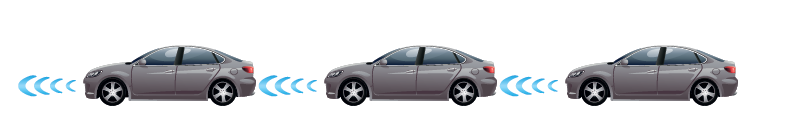
\includegraphics[width=1\textwidth]{figures/vehiclePlatoonusingACC.png}
    \centering
    \caption{Vehicle platoon using ACC}
    \label{fig:Vehicle Platoon using ACC}    
\end{figure}

\begin{figure}[h!]
    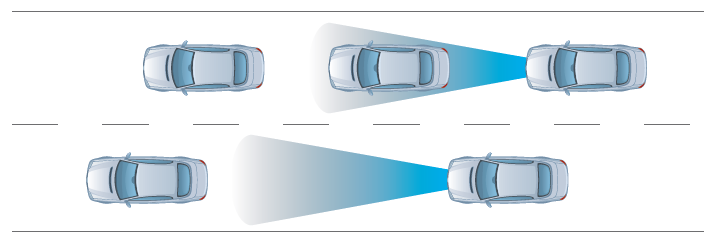
\includegraphics[width=1\textwidth]{figures/typicalviewoffrontradarusingACC.png}
    \centering
    \caption{A typical view of a front-radar used in ACC}
    \label{fig:A typical view of a front-radar used in ACC}    
\end{figure}

\begin{figure}[h!]
    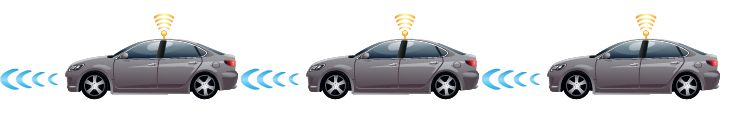
\includegraphics[width=1\textwidth]{figures/vehicleplatooningusingCACC.png}
    \centering
    \caption{Vehicle platoon using CACC}
    \label{fig:vehicleplatooningusingCACC}    
\end{figure}

\subsubsection{Cooperative Adaptive Cruise Control}
CACC augments ACC with wireless communication, new control logic and GPS as illustrated in Figure \ref{fig:vehicleplatooningusingCACC}. Wireless communication allows vehicles to extend their view beyond the LOS of the radar. With CACC, the third vehicle in the illustration of Figure \ref{fig:vehicleplatooningusingCACC} is notified via wireless communication of the behavior of the leading vehicle. The third vehicle can almost instantly react to speed changes of the first vehicle and as a result, a CACC system enables to drive with closer headways.

\subsubsection{Automated Highway System (AHS)}
With both ACC and CACC, the driver is (partly) responsible for the operation of the vehicle. The driver is for example still responsible for steering the vehicle. The next step in vehicle platooning is a system in which vehicles are fully automated. AHS platoons are similar to CACC platoon as illustrated in Figure \ref{fig:vehicleplatooningusingCACC}. However, AHS platoons rely heavily on wireless communication to create automated and high cooperative vehicles.

\subsubsection{Advantages and Risks of Platooning}
The advantages of vehicle platooning include \cite{de1997behavioral} an increase in road capacity, reduction of environmental impacts, improved safety, improved driver comfort, highly cooperative groups, decrease in fuel consumption (reduced air resistance), shorter commutes during peak periods, etc. 

The risks of platooning include the driver is less in control being at the hands of computer software or lead driver and the driver is inattentive than usual hence not able to react as quickly to adverse situations if software or hardware fails.

\subsubsection{Vehicle Platooning Control Functions}
The most basic functionality for automated vehicles in vehicle platoons, being respectively longitudinal control, lateral control and maneuver control \cite{shladover2005automated}.

Longitudinal control of a vehicle is the feature that controls the speed and distance to the preceding vehicle using powertrain and brakes. Implementations of the longitudinal control rely heavily on measurements of headway and the speed of the preceding vehicle. Longitudinal controllers that control the speed of a vehicle, purely based on the vehicle's sensors are classified as autonomous. Autonomous controllers are capable of maintaining string stability i.e. headway errors do not flow down the platoon, under constant time gaps between vehicles. Another type of longitudinal control is cooperative control. These controllers typically complement radar and image-processing sensors with wireless communication to collect state information (position, speed, acceleration, and maneuver information) of close operating vehicles. These type of controllers are not only able to maintain string stability under constant time gap, like autonomous controllers, but also under constant distance gaps.

The primary functionality of lateral control is keeping the vehicle in the center of the lane. Lateral control is also concerned with lane changing wherein lane changing is the feature to steer a vehicle from the current lane to an adjacent lane.

Vehicle platooning involves, apart from longitudinal and lateral control, the coordination of vehicle maneuvers. These maneuvers are typically the formation and splitting of platoons, the merging of traffic streams and coordination of changing lanes.\\

Additional details on platooning and its implementation can be obtained by referring to SARTRE Report on Fuel Consumption, SARTRE Report on Infrastructure and Environment, \cite{bergenhem2010challenges}, \cite{chan2012cooperative}, \cite{davila2010sartre}, etc.

\section{Vehicular RF Channel} 
Key characteristics of vehicular channels are shadowing by other vehicles, high Doppler shifts, and inherent non-stationarity \cite{mecklenbrauker2011vehicular}. All have a major impact on the data packet transmission reliability and latency. For vehicular channels, it is customary to distinguish between V2V and V2I channels. These channels not only
differ from each other but also deviate significantly from those in cellular communication. In cellular scenarios, the base station (BS) is fixed, elevated, and located at or above rooftop level, such that its close surroundings are free of scatterers. Furthermore, most of the relevant scatterers are
immobile or move relatively slowly. The distance between the BS and the user span roughly from 10 m to 10 km. In a V2V communication scenario, there is neither an access point (AP) nor BS and both the Rx and the Tx may move with high velocities. The antennas are mounted at a the height of 1-2 m, many relevant scatterers (i.e., vehicles) move, and the distances between the Tx, the Rx, and principal scatterers are in the range of a few hundred meters. Depending on whether the scenario includes a the road in an open field or a busy street in an urban environment, the number of relevant scatterers might vary significantly.

The following five properties mainly characterize wireless channels.
\begin{itemize}
    \item Pathloss: How does the average received power level vary with distance to the transmitter?
    \item Signal fading: How does the instantaneous signal level fluctuate over time, frequency, and space?
    \item Delay spread: How is the signal smeared in time by echoes?
    \item Doppler spread: How is the transmitted signal smeared in frequency due to movements of the Rx, the Tx, and scatterers?
    \item Angular spread: How is the transmitted signal smeared over directions by antennas and scatterers?
\end{itemize}

The propagation conditions in particular for V2V communications
are influenced by the antennas and their placement on the vehicle. The roof of the vehicle can strongly affect the antenna pattern; if the antenna is placed on a backward-slanted roof, it has difficulties seeing vehicles in front of it.

The region over which the transmitter provides coverage is smaller than the area in which it creates interference. Due to high speeds involved, V2V channels show substantial time variance (the channel state changes) and non-stationarity (the channel statistics change). These effects are more pronounced for cars approaching each other or approaching intersections, while they are less severe for vehicles driving in convoys or V2I communications.

\section{WiFi-p}
An international standard, IEEE 802.11p \cite{ieee1997wireless}, which is part of the WAVE initiative, has gained considerable importance. Based on popular WiFi standard, it is intended for both V2I and V2V traffic telematics applications and operates in the 5.9-GHz band. Its importance is further highlighted by the European decision on the use of the 5875-5905 MHz frequency band for safety-related ITS applications \cite{reding2007commission}. IEEE 802.11p is an amendment to the IEEE 802.11 standard for vehicular networks. Modifications to the original standard were needed as the MAC, and PHY layers were never designed for mobile environments. We note that a 700 MHz band is devoted to advanced driving safety support systems in Japan \cite{mecklenbrauker2011vehicular}. IEEE 802.11p is also one mode of communication access for land mobiles, a framework for heterogeneous packet-switched communication in mobile environments approved by the International Standards Organization (ISO). Summarizing, the IEEE 802.11p standard has established itself as the key technology for V2V and safety-critical V2I communications.

Figure \ref{fig:DSRC spectrum band and channels} shows the DSRC spectrum band and its channels as allocated by the FCC. This allocation consists of 7 channels with a bandwidth of 10 MHz each. Some of these channels are restricted to be used for the transmission of a particular type of information. For instance, channel 178 is the control channel and can only be utilized for the transmission of safety-related data. The outer channels number 172 and 184 are reserved for special purpose communication, and the remaining four channels can be used for both safety and non-safety related communication \cite{chen2009ieee}.


\begin{figure}[h!]
    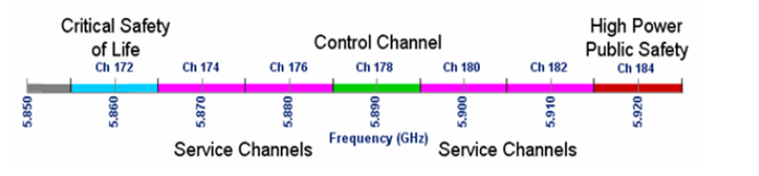
\includegraphics[width=1\textwidth]{figures/DSRC spectrum band and channels.png}
    \centering
    \caption[DSRC spectrum band and channels]{DSRC spectrum band and channels \protect\cite{chen2009ieee}}
%    \protect\citeA{chen2009ieee}
    \label{fig:DSRC spectrum band and channels}    
\end{figure}



\section{UWB}
UWB differs substantially from conventional narrowband radio frequency (RF) and spread spectrum technologies (SS), such as Bluetooth Technology and 802.11 a/g. UWB uses an extremely wide band of RF spectrum to transmit data as shown in Figure \ref{fig:Comparision of narrowband, spread spectrum, and ultra-wideband signal concepts}.

\begin{figure}[h!]
    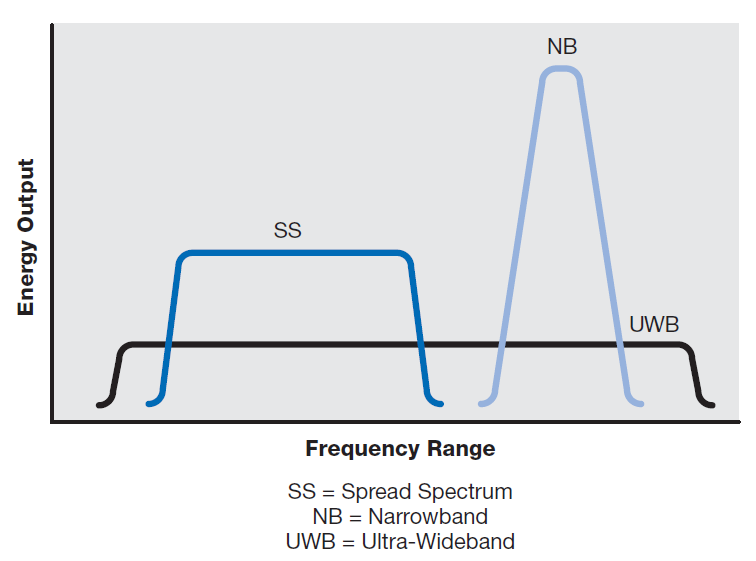
\includegraphics[width=0.7\textwidth]{figures/UWBcomparedtoNB.png}
    \centering
    \caption[Comparision of narrowband, spread spectrum, and ultra-wideband signal concepts]{Comparision of narrowband, spread spectrum, and ultra-wideband signal concepts   \protect \cite{IntelUWB}}
 
    
    \label{fig:Comparision of narrowband, spread spectrum, and ultra-wideband signal concepts}    
\end{figure}

The potential data rate over a given RF link is proportional to the bandwidth of the channel and the logarithm of the signal-to-noise ratio (Shannon’s Law) \cite{haykin2008communication}. RF design engineers typically have little control over the bandwidth parameter, because this is dictated by FCC regulations that stipulate the allowable bandwidth of the signal for a given radio type and application. Bluetooth technology, 802.11a/g Wi-Fi, cordless phones, and numerous other devices are relegated to the unlicensed frequency bands that are provided at 900 MHz, 2.4 GHz, and 5.1 GHz. Each radio channel is constrained to occupy only a narrow band of frequencies, relative to what is allowed for UWB.

UWB is a unique and new usage of a recently legalized frequency spectrum. UWB radios can use frequencies from 3.1 GHz to 10.6 GHz - a band more than 7 GHz wide. Each radio channel can have a bandwidth of more than 500 MHz, depending on its center frequency. To allow for such a large signal bandwidth, the FCC put in place severe broadcast power restrictions. By doing so, UWB devices can make use of an extremely wide frequency band while not emitting enough energy to be noticed by narrower band devices nearby, such as 802.11a/g radios \cite{karapistoli2010overview}. Figure \ref{fig:IEEE 802.15.4a UWB Frequency Bands} denotes the center frequencies and bandwidths of the defined bands, as well as the regulatory domains in which they are admissible. Frequency bands (channel numbers) 4, 7, 11, 15 have the same center frequency as bands 2, 5, 9, 13 respectively. This is due to the fact that bands 4, 7, 11, 15 are all "wide-band" channels whose bandwidth is larger than 1 GHz, and these bands, in fact, overlay the other 500 MHz wide bands.

\begin{figure}[h!]
    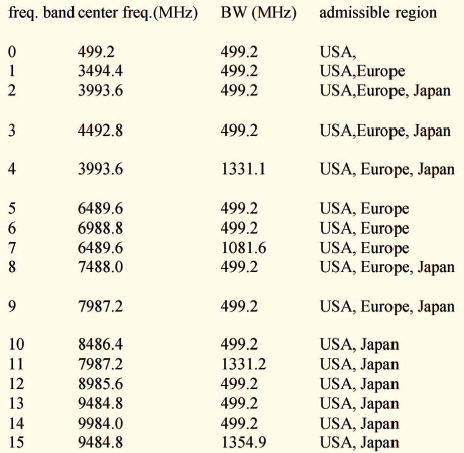
\includegraphics[width=0.8\textwidth]{figures/uwbchannels.png}
    \centering
   \caption[IEEE 802.15.4a UWB Frequency Bands]{IEEE 802.15.4a UWB Frequency Bands \protect\cite{zhang2009uwb}}
%    \protect\citeA{zhang2009uwb}
    \label{fig:IEEE 802.15.4a UWB Frequency Bands}    
\end{figure}

UWB communications are based on the transmission and reception of frames. Figure \ref{fig:UWB PHY Frame structure} shows the general structure of the UWB frame. It begins with a synchronization header consisting of the preamble and the Start of the Frame Delimiter (SFD), after which the PHY header (PHR) defines the length (and data rate) of the data payload part of the frame.

\begin{figure}[h!]
    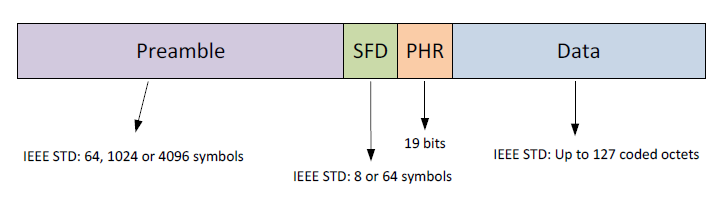
\includegraphics[width=0.8\textwidth]{figures/UWBPHYFrameStructure.png}
    \centering
    \caption[UWB PHY Frame structure]{UWB PHY Frame structure \protect\cite{DW1000UserManual}}
%    \protect\citeA{DW1000UserManual}
    \label{fig:UWB PHY Frame structure}    
\end{figure}

\begin{figure}[h!]
    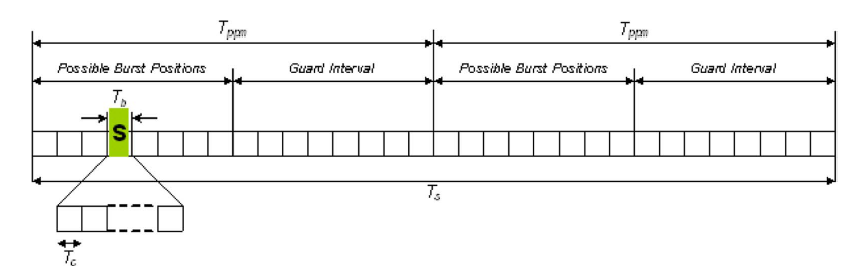
\includegraphics[width=0.8\textwidth]{figures/ModulationandTimehoppingof802.15.4a.png}
    \centering
    \caption[UWB Symbol duration]{UWB Symbol duration \protect\cite{gutierrez2004low}}
%    \protect\citeA{gutierrez2004low}
    \label{fig:UWB Symbol duration}    
\end{figure}

Figure \ref{fig:UWB Symbol duration} shows the UWB Symbol duration, $T_c$ is the chip (pulse) duration of approximately 2 ns, $T_b$ is the burst-hopping duration, which equals, $T_b$ = N$T_c$ = 32 ns, n indexes the N=16 pulses that are transmitted during each data burst. $T_{ppm}$ is the modulation interval for the pulse position modulation $T_{ppm}$ = 16$T_b$, and $T_s$ is the symbol duration.

The UWB used in 802.15.4 is also called impulse radio UWB because it is based on high-speed pulses of RF energy. During the PHR and data parts of the frame, information bits are signaled by the position of the burst, in a modulation scheme termed Burst Position Modulation (BPM). Each data bit passes through a convolution encoder to generate a "parity bit" used to set the phase of the burst as either positive or negative, this component of the modulation is termed binary phase-shift keying (BPSK). 

Also, the quarter symbol interval is sub-divided into 2, 4, or 8 sub-intervals and a pseudo random sequence used to determine both the burst shape and which of the sub-intervals are used for the burst transmission. This gives more immunity to interference and whitens the output spectrum allowing a higher signal power to be utilized in the transmitter.


To ensure that the signals can still be decoded by noncoherent receivers, a systematic code is used wherein the systematic code is one in which the information bits are transmitted unchanged along with the parity check bits. The systematic bits are used to determine the PPM position of the burst and are visible to both noncoherent and coherent receivers. The parity bits are modulated onto the burst phase and are thus visible only to coherent receivers. Forward error correction (FEC) is also included in the PHR and data parts of the frame. The 19-bit PHR includes a 6-bit Single-Error-Correct-Double-Error-Detect (SECDED) code and the data part of the frame has a Reed-Solomon (RS) code applied. Both SECDED and RS codes are systematic \cite{zhang2009uwb}.

The synchronization header consists of the preamble sequence and the SFD. In contrast to the BPM/BPSK modulation used for the PHR and data, the synchronization header is made up of single pulses. The symbol is divided into approximately 500 "chip" time intervals, (496/508 depending on 16/64 MHz PRF), in which either a negative or a positive pulse may be sent, or no pulse. The "chip" interval is 499.2 MHz, a fundamental frequency within the UWB PHY, and so the resultant symbol times are thus 496/499.2 us for 16 MHz PRF, 508/499.2 us for 64 MHz PRF. It is to be noted that number of chips per burst change for PRF of 16 or 64 MHz. The number of chips per burst for 64 MHz PRF will be four times greater than the number of chips per burst for 16 MHz PRF  \cite{gutierrez2004low}.

The sequence of pulses sent during the symbol interval is determined by preamble code. The standard defines eight different length-31 preamble codes for use at 16 MHz PRF and 16 different length-127 preamble codes for use at 64 MHz PRF. 

The standard nominates particular codes for specific channels so that at 16 MHz PRF there are just two to choose from per channel, while at 64 MHz PRF there is a choice of four codes per channel. The length-31 codes are spread by inserting 15 zeros for each code point to give the 496 chip times per symbol while the length-127 codes are spread by adding three zeros for each code point to give the 508 chip times per symbol. The preamble length is defined by how many times (i.e. for how many symbols) the sequence is repeated. This is determined by the configuration of Preamble Symbol Repetitions (PSR).

The standard defines PSR settings of 16, 64, 1024 and 4096. The preamble sequence has a property of perfect periodic autocorrelation \cite{ipatov1979ternary} which in essence allows a coherent receiver to determine the exact impulse response of the RF channel between transmitter and receiver. This brings two significant benefits. Firstly, it allows the receiver to make use of the received energy from multiple paths, turning multipath from an interference source into a positive affect extending operating range. Secondly, it lets the receiver resolve the channel in detail and determine the arrival time of the first (most direct) path, even when attenuated, which brings precision advantages for Real Time Location System (RTLS) applications. 
The SFD marks the end of the preamble and the precise start of the switch into the BPM/BPSK modulation of the PHR. The time-stamping of this event is very deterministic in terms of symbol times, and it is this in conjunction with determining the first arriving ray within that symbol time that allows the accurate time-stamping needed for precision RTLS applications.

The standard specifies the SFD, which consists of the preamble symbols either not sent, or sent as normal or sent inverted (i.e. positive and negative pulses reversed) in a defined pattern eight symbol times long for data rates other than 110 kbps, and 64 symbols long for the 110 kbps mode.

The PHY header (PHR) is modulated using the BPM/BPSK modulation scheme, but it does not employ the Reed-Solomon code used for data, instead is employs a 6-bit SECDED parity check sequence as part of its 19-bit length.

The preamble codes specified by the standard for use on a particular channel were chosen to have a low cross-correlation factor with each other with the intention that the complex channels could operate independently from each other as separate networks.

The IEEE 802.15.4 UWB PHY standard includes a feature called Dynamic Preamble Select (DPS) intended for use in a security mechanism for two-way ranging, where devices switch to using one of the DPS specific preamble codes for the ranging exchange, and perhaps a different one for each direction of communication. The idea is to make it harder to eavesdrop or spoof, by randomly changing the DPS preamble codes in a mutually agreed sequence only known to the valid participants.


\section{UWB Ranging}
In all of the schemes that follow one node acts as Initiator, initiating a range measurement, while the other node acts as a Responder listening and responding to the initiator, and calculating the range. 

Single-sided two-way ranging (SS-TWR) involves a simple measurement of the round trip delay of a single message from one node to another, and a response sent back to the original node. 

\begin{figure}[h!]
    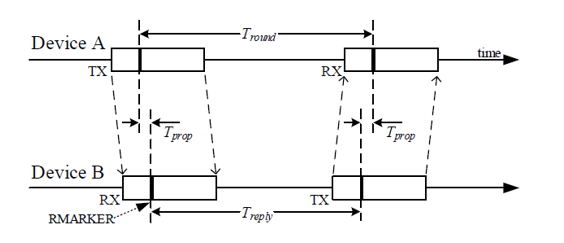
\includegraphics[width=0.8\textwidth]{figures/SSTWR.png}
    \centering
    \caption[Single-sided Two-way ranging]{Single-sided Two-way ranging \protect\cite{DW1000UserManual}}
%    \cite{DW1000UserManual}
    \label{fig:Single-sided Two-way ranging}    
\end{figure}

The operation of SS-TWR is as shown in Figure \ref{fig:Single-sided Two-way ranging}, where device A initiates the exchange and device B responds to complete the exchange and each device precisely timestamps the transmission and reception times of the message frames, and so can calculate times $T_{round}$ and $T_{reply}$ by simple subtraction.  And the resultant time-of-flight, $T_{prop}$ may be estimated by the equation:  
\begin{equation}
 T_{prop} = 0.5 (T_{round} - T_{reply})
\end{equation}

The times $T_{round}$ and $T_{reply}$ are measured independently by device A and B using their respective local clocks, wherein both have some clock offset error eA and eB from their nominal frequency, and so the resulting time-of-flight estimate has a considerable error that increases as $T_{reply}$ increases.  Depending on the size of ranging error that is acceptable to the application, SS-TWR may be an appropriate choice for range measurement especially if the reply time $T_{reply}$ is minimized and the clock error is low.  It should be noted that the reply time $T_{reply}$ is not just the RX-to-TX turnaround time but also includes the message length. 

It can be seen that as $T_{reply}$ increases and as the clock offset increases the error in the time-of-flight estimation increases to the point where the error is such as to render the estimation very inaccurate.  For this reason, SS-TWR is not commonly used, but it is worthy of examination for particular use cases where tight tolerance clocks are used, and the communication range is relatively short \cite{gutierrez2004low}.

Double-sided two-way ranging (DS-TWR), is an extension of the basic single-sided two-way ranging in which two round trip time measurements are used and combined to give a time-of-flight result which has a reduced error even for quite long response delays.  The operation of DS-TWR is as shown in Figure \ref{fig:Double-sided Two-way ranging}, where device A initiates the first round trip measurement to which device B responds, after which device B starts the second round trip measurement to which device A responds completing the full DS-TWR exchange.  Each device precisely timestamps the transmission and reception times of the messages. The four messages of DS-TWR, shown in Figure \ref{fig:Double-sided Two-way ranging}, can be reduced to three messages by using the reply of the first round-trip measurement as the initiator of the second round-trip measurement. The resultant time-of-flight estimate, $T_{prop}$, in both the three and four message cases may be calculated using the expression: 
\begin{equation}
T_{prop}=(T_{round1} \times T_{round2}-T_{reply1} \times T_{reply2})/(T_{round1}+T_{round2}+T_{reply1}+T_{reply2})
\end{equation}



\begin{figure}[h!]
    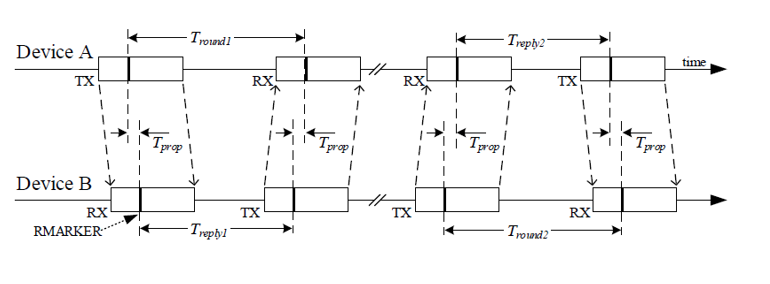
\includegraphics[width=0.8\textwidth]{figures/DSTWR.png}
    \centering
    \caption[Double-sided Two-way ranging]{Double-sided Two-way ranging \protect\cite{DW1000UserManual}}
%    \cite{DW1000UserManual}
    \label{fig:Double-sided Two-way ranging}    
\end{figure}

Both of the above schemes are denoted ASYMMETRIC because they do not require the reply times from each device to be the same.   
Using this scheme, the typical clock induced error is in the low picosecond range even with 20 ppm crystals. At these error levels, the precision of determining the arrival time of the messages at each of the receivers is a more significant contributor to overall $T_{prop}$ error than the clock-induced error. 

There is a special case of the double sided scheme known as SYMMETRIC Double-sided Two-way ranging in which $T_{reply1}$ and $T_{reply2}$ are restrained to be equal (or as close to equal as possible).  In this case: 

\begin{equation}
T_{prop}=(T_{round1} - T_{reply2} + T_{round2} + T_{reply1})/4
\end{equation}

This scheme requires only addition, subtraction, and division by four which is easily achieved in low power microcontrollers however it results in the entire exchange taking longer than necessary. 

The sources of error for ranging include Clock drift, Frequency drift, $T_{reply}$ (turnaround time from receiver to transmitter or vice versa, including the time required for creation of message), ranging transaction performed while one of the devices is transitioning through the crystal warm-up phase (during duty cycling) and bias which varies with received signal strength.

\section{LPCXpresso4337 development board}
The LPCXpresso4337 board {\cite{LPCUserManual}} has been developed by NXP to enable evaluation of and prototyping with the LPC4300 family of MCUs and features the LPC4337 in its 100 PIN BGA package option. LPCXpresso is a low-cost development platform available from NXP supporting NXP's ARM-based microcontrollers. The platform is comprised of a simplified Eclipse-based IDE and low-cost target boards which include an attached SWD debugger. LPC4337 has a dual core (M4 and M0) MCU running at up to 208 MHz. It includes up to 264 KB of SRAM. 
The LPCXpresso4337 board includes the following features: 
\begin{itemize}
    \item On-board, high-speed USB based, Link2 debug probe with support for ARM’s CMSIS-DAP, LPCXpresso IDE Redlink and SEGGER J-Link protocol options 
    \item Link2 probe can be used with on-board Target MCU or external target 
    \item Support for external debug probes 
    \item Tri-color LED 
    \item Target Reset, ISP and WAKE buttons 
    \item Expansion options based on Arduino UNO and PMod, plus additional expansion port pins 
    \item UART, I2C, and SPI port bridging from Target MCU to USB via the on-board debug probe 
    \item UART connector 
\end{itemize}

More information about the peripherals available on the chip can be found in the user manual \cite{LPCUserManual}.

\section{DecaWave DW1000}
DW1000 \cite{DW1000UserManual} is an IEEE 802.15.4-2011 UWB compliant wireless transceiver module. Its features include high data rate communications, low power consumption, small physical size, highly immune to fading, etc. The DecaWave DW1000 transceiver is embedded on to the LPCXpresso4337 board. It spans 6 RF bands from 3.5 GHz to 6.5 GHz and supports data rates of 110 kbps, 850 kbps, and 6.8 Mbps.

The DW1000 consists of an analog front-end (both RF and baseband) containing a receiver and transmitter and a digital backend that interfaces to a host processor, controls the analog front-end, accepts data from the host processor for transmission and provides received data to the host processor over an industry standard SPI interface. 

The DW1000 provides capabilities to take accurate transmission timestamp, supports delayed transmission, extended length data frames, cyclic redundancy check, frame filtering, automatic acknowledgment, automatic receiver re-enable, etc.

DW1000 supports Smart transmit power control. The power output regulations typically specify limits as -41 dBm in each 1 MHz bandwidth and generally measure this using a 1 ms dwell time in each 1 MHz segment.  When sending short frames at 6.8 Mbps, it is possible for a single frame to be transmitted in a fraction of a millisecond. So long as the transmitter does not transmit again within that same millisecond, the power of that transmission can be increased while complying with the regulations.  This power increase will increase the transmission range. Smart TX power control acts at the 6.8 Mbps data rate. DW1000 allows operating using different channels, preamble codes, preamble lengths, with Standard SFD or non-standard SFD, PRF, etc.

More information about DW1000 can be found in the datasheet \cite{DW1000DataSheet} and user manual \cite{DW1000UserManual}.
\clearemptydoublepage

\chapter{Related Work}\label{chapter:relatedWork}
\nomenclature[A]{SIC}{Successive Interference Cancellation}
\nomenclature[A]{BER}{Bit Error Rate}
\nomenclature[A]{UMTS}{Universal Mobile Telecommunication System}
\nomenclature[A]{CSMA}{Code Division Multiple Access}
\nomenclature[A]{EIRP}{Equivalent Isotropically Radiated Power}
\nomenclature[A]{SIR}{Signal to Interference Ratio}
\nomenclature[A]{DAA}{Detect and Avoid}
\nomenclature[A]{IVC}{Inter-vehicle Communication}

In Section 3.1, we present the related work about the use of UWB for inter-vehicle communication, interference of UWB to other narrowband communication protocols and vice-versa, and UWB Ranging. In Section 3.2, we highlight the novel aspects of the current work.

\section{Summary}
There have been several studies conducted on UWB radars for inter-vehicle communication, interference of UWB on other narrowband communication protocols and vice-versa, the coexistence of UWB with other narrowband communication protocols and UWB ranging as indicated below.

\subsection{UWB for inter-vehicle communication}

The authors of \cite{kohno2008latest} state that UWB is a promising technology for both communications and ranging in highly reliable systems such as ITS and medical healthcare. The authors of \cite{sakkila2008uwb} propose a road radar to be embedded on the vehicles based on UWB technology which provides good resolution and increased precision for detection and localization of obstacles, attributed to the high degree of accuracy that UWB provides and its capability to differentiate between various obstacles like cars, plates, pedestrians, etc. The authors of \cite{doi2004frequency} propose an inter-vehicle UWB radar system using chirp waveforms instead of the conventional UWB-IR system that uses a modulated Gaussian pulse wherein the transmitted signal consists of a linear combination of chirp signals with the same time duration but different frequency bands. They show that this system has a lower non-detected rate than the conventional UWB-IR system, and hence suitable for ITS applications. 

The authors of \cite{takahara2012study} propose a UWB radar system assisted by communication to improve safety by obtaining additional information of the target vehicle by communication. They show that it is possible to improve the precision of ranging against the distant vehicles by following this approach through computer simulations. In the proposed scheme, the data for communication is appended to the UWB radar signal and the preceding target vehicle that receives the radar signal obtains information of the following vehicle. Moreover, the target vehicle transmits its driving information to the following vehicle after specific time duration. The following vehicle receives not only the reflected radar signal but also the following communication signal from the target vehicle. By using these two signals, more precise ranging and information collection can be performed. They indicate that in a conventional UWB radar, the precision of ranging usually degrades against distant targets because of degradation of the signal to noise ratio of the reflected signal from the target vehicle. However, using the proposed scheme, it is possible to improve ranging precision by detecting the communication signal that is transmitted just after the reflected signal from the target vehicle. 

In \cite{takahara2013study}, the authors discuss the problems encountered as a result of the proposed system presented above. They state that near-far problem due to the difference of signal power from each vehicle and inter-symbol interference while communicating with multiple devices was encountered and propose an iterative detection system using Successive Interference Cancellation (SIC) to improve the detection rate of the signal and the bit error rate (BER) performance. In the iterative detection system, the signals except the desired signal detected by SIC is subtracted from the original received signal leading to improved performance in simulations. The authors of \cite{takahara2014study} determine that the data to be transmitted through communication should include vehicle ID and the transmission time of the signal.

The authors of \cite{elbahhar2005using} propose an inter-vehicle communication system based on UWB. They study two types of UWB waveforms: coded Gaussian and monocycle pulses and state that Gaussian pulses waveform was the better of the two since the obtained BER was lower than that for monocycle pulses during simulations.

\subsection{Interference of UWB on narrowband communication and vice-versa}
In \cite{hamalainen2003ultra}, the authors investigated the level of impact of UWB devices on IEEE 802.11b and Bluetooth networks using a UWB device corresponding to hundreds of FCC-compliant UWB devices because of its high transmitted power level, in the 2.4-GHz ISM band. They state that under the extreme interference conditions examined, the UWB devices can have an impact on both IEEE 802.11b and Bluetooth networks, depending on the separation from the victim system. For interference distances of less than 50 cm, the UWB interferers affected the reported SNR for both LOS and NLOS cases. The worst case degradation of the received SNR in the IEEE 802.11b was less than 15 dB for 20 UWB devices (equivalent to several thousand FCC-complaint UWB devices) at 10 cm distance. A corresponding drop in the network throughput was observed only for the NLOS case and only for distances of less than 35 cm. In the LOS case, the impact of the UWB devices was insignificant. With respect to the Bluetooth connection, they state that it does not suffer significantly from the UWB interferers. The resulting decrease in throughput was approximately 20 Kbps in the worst case.

The authors of \cite{sadowski2011narrowband} measured the narrowband transmission quality in the presence of impulse radio UWB interference with unmodified IEEE 802.15.4a and modified IEEE 802.15.4a IR UWB signal. They state that selective reduction of UWB power spectral density at the frequency of narrowband transmission allowed to reduce bit error rate without the need to decrease the power of UWB interferer. 

In \cite{findikli2011performance}, the authors assess the UWB-IR system performance in the presence of an active narrow-band system. They show that while the BER performances of coherent and non-coherent receiving structures may be slightly degraded with the use of a linear combination of pulses when there is no active narrow-band system, the performances can be significantly improved with appropriate filtering techniques at the receiver when a narrow-band system is active. The authors of \cite{taha2002theoretical} state that interference coming from external sources degrade the UWB radio performance and depending on the frequency of narrowband interferers, they degrade the performance differently. They state that those narrow band interferers with frequencies concentrated at regions where the UWB radio pulse has stronger frequency contents, degrade the performance more severely. Moreover, they state that careful design of UWB pulse shape can mitigate the narrowband interference.

In \cite{ahmed2008impact}, the authors assess the effect of UWB on the Universal Mobile Telecommunication System (UMTS) and Code Division Multiple Access systems (CSMA-450). They show that, for the case of a single UWB transmitter, the UMTS can easily tolerate UWB interference when the UWB Equivalent Isotropically Radiated Power (EIRP) is -92.5 dBm/MHz or less for a distance between the UWB transmitter and the UMTS mobile of 1 m or higher. Also, they show that, for the case of multi-UWB transmitters, the UMTS can easily tolerate the UWB interference when the UWB EIRP is -94.5 dBm/MHz. For the single UWB transmitter case, the CDMA-450 downlink can tolerate UWB interference when the UWB power density is in the order of -106 dBm/MHz. For the case of multi-UWB transmitters, the power density that can be tolerated by the downlink of the CDMA-450 system is in the order of -108 dBm/MHz.

In \cite{chiani2009coexistence}, the authors assess the coexistence between UWB and narrowband wireless communication systems. Concerning UWB systems affected by narrowband interference, they show that the impact of narrowband interference strongly depends on, for a UWB-IR coherent receiver, on the carrier frequency of the interferer, the UWB pulse shape, and the spreading code adopted. They found that there was no significant performance degradation in the UWB link for Signal to Interference Ratio (SIR) on the order of -20 dB or greater. However, they state that the low transmitted power level currently allowed for UWB systems, which is typically much lower than that for narrowband transmitters could lead to a scenario wherein strong narrowband interferers could produce very small SIR at the UWB receiver. Similarly, for the dual case of narrowband systems affected by UWB interference, they show that the effects of a single UWB interferer are almost negligible, and the performance of the narrowband links are practically unchanged for sufficiently large SIR values. However, they state that in situations where the narrowband receiver is much closer to the UWB transmitter than to narrowband transmitter, can lead to very low SIR, with a consequent performance degradation in the narrowband link.

The authors of \cite{lewandowski2010coexistence} examine the coexistence of 802.11b and 802.15.4a-CSS through simulations and show that an error free coexistence of IEEE 802.11b and IEEE 802.15.4a-CSS is not feasible. The authors of \cite{mishra2007detect} show that in their UWB/WiMax coexistence experiments conducted by using a single UWB device with WiMax system, it is indeed feasible for UWB and WiMax system to co-exist by using Detect and Avoid (DAA) mechanism.

\subsection{UWB Ranging}

In \cite{soganci2011accurate}, the authors observe that time-based ranging is well suited for UWB systems. In \cite{lanzisera2009rf}, the authors tested outdoor ranging using two Waldo nodes in a parking lot with some cars but mostly open space. The environment was providing a baseline for ranging performance in an atmosphere where there is relatively little multipath interference. The method of communication between the nodes was through a wireless link. Range estimates were taken at distances ranging from 1 m to 45 m, and the received signal strength estimates were considered as well. They found that the received signal strength range estimates did not provide good range estimates compared to the time of flight estimates even in a mild multipath environment, but the time of flight measurements performed much better. They found that approximately 80\% of the time of the flight measurements were accurate to within 1 m, but not even 20\% of the received signal strength based estimates were within 1m. The authors of \cite{kristem2014experimental} carried out UWB ranging measurement in a dense urban environment at distances of 20 m,30 m, and 40 m, with two different antenna heights. They observed that the root mean square error in the range increased from 0.12 m to 0.14 m for LOS measurements and from 7.9 m to 9.8 m in NLOS measurements when the antenna height reduced from 100 cm to 10 cm.

The authors of \cite{petovello2012demonstration} propose the concept of differential GPS relative navigation augmented with UWB and bearing measurements. They found that combining GPS pseudo range, UWB range, and bearing measurements can significantly improve horizontal positioning accuracy, particularly in environments where GPS availability is reduced. The UWB measurements contributed to an improved along-track relative position while the bearing measurements improved the across-track position. 

The authors of \cite{ye2011experimental} examine the effect of LOS and NLOS ranging in indoor and outdoor environments using IEEE 802.15.4a impulse UWB transceiver. They found that the average ranging error was less than 20 cm when measured outdoors for a distance of 10 m in LOS. In the NLOS case, they found that the ranging error varied from 6 cm (Glass) to 29 cm (Door) when measured with a 3 m testing point.

\section{Novelty}
In this Section, we describe the limitations of the existing work and the novel aspects of our work in the field of inter-vehicle communication.

\subsubsection{Limitations}
\begin{enumerate}
	
	\item Interference of UWB to WiFi-p or vice-versa has not been studied.
	\item The influence of Channel, Preamble length, PRF, Standard SFD, Non-standard SFD, Smart Power enablement, Preamble code on UWB link in the presence of WiFi-p interference has not been studied.
	\item The feasibility of using UWB as a secondary independent backup channel for platooning has not been studied.
	\item The performance of IR-UWB link in the presence of speed or acceleration difference has not been documented.
	\item Effect of speed or acceleration on ranging accuracy with respect to platooning has not been documented.
	\item Existence of UWB Nulls has not been documented.
	\item Effect of Standard SFD and Non-standard SFD on ranging accuracy has not been documented.
	\item UWB for Inter-Vehicle Communication (IVC) has been evaluated only through UWB radars and simulations. UWB communication for IVC through actual experiments has not been documented.
\end{enumerate}

IEEE 802.15.4a is a relatively new standard, which has not been tested in an inter-vehicle and outdoor environment for platooning. This thesis focuses on handling all the above limitations except limitation 5. We design a set of measurement goals in Chapter 4 to study the feasibility of using UWB as a secondary independent backup channel for platooning. We implement a test platform (Chapter 5) to study the measurement goals in different test set-ups. We study the LDC requirements of UWB in (Chapter 6). We conduct experiments (Chapter 7) in various test set-ups under different experimental scenarios and analyze the outcomes to study the above-mentioned measurement goals.


\clearemptydoublepage

\chapter{Test Platform Requirements}\label{chapter:testPlatformRequirements}
\nomenclature[A]{VFM}{Vehicle Following Message}
\nomenclature[A]{PSM}{Platoon Status Message}
\nomenclature[A]{PRR}{Packet Reception Ratio = 100 - PER}
\nomenclature[A]{CSS}{Chirp Signal Spectrum}
\nomenclature[A]{LOS}{Line Of Sight}
\nomenclature[A]{CIRP}{Channel Impulse Response Power}
\nomenclature[A]{PAC}{Preamble Accumulation Count}

In Section 4.1, we define the link quality metrics used for our experimental analysis.
In Section 4.2, we list the set of goals to determine the suitability of using UWB as a secondary independent backup channel for platooning derived from our research questions. In Section 4.3, we explain the role of both the nodes in the network. In Section 4.4, we describe the data communication primitive that will be used to study the link quality. In Section 4.5, we design measurement plans. In Section 4.6, we list the set of requirements of the test platform TP-UWB that enables us to execute the developed measurement plans. In Section 4.7, we list the set of post-processing requirements.

\section{Communication Performance Metrics}
Below we define the various metrics that we use to perform the comparative analysis of different configurations.

\subsection{Packet Error Ratio}
The Packet Error Ratio gives a measure of the relative number of packets lost in a link. We define the following variables:
\begin{itemize}
    \item A = Total number of packets transmitted by the leading truck during the data communication state at the link layer.
    \item B = Total number of packets received by the following truck during the data communication state at the link layer.
    \item C = Total number of packets transmitted by the following truck during the data communication state at the link layer
    \item D = Total number of packets received by the leading truck during the data communication state at the link layer.
    
    We define the packet error ratio (PER) of the leading truck and the following truck using the above variables.
    
    \begin{equation}
    PER_{LeadingTruck} = (C-D)/C
    \label{eq: PERLeadingTruck}
    \end{equation}
    \begin{equation}
    PER_{FollowingTruck} = (A-B)/A
    \label{eq: PERFollowingTruck}
    \end{equation}
    
\end{itemize}

\subsection{Message Error Ratio}
The Message Error Ratio gives a measure of the relative number of messages lost in a link wherein a message is a combination of several packets. We define the following variables:
\begin{itemize}
    \item A = Total number of messages transmitted by the leading truck during data communication state at the application layer.
    \item B = Total number of messages received by the following truck during data communication state at the application layer.
    \item C = Total number of messages transmitted by the following truck during data communication state at the application layer
    \item D = Total number of messages received by the leading truck during data communication state at the application layer.
    
    We define the Message Error Ratio (MER) of the leading truck and the following truck using the above variables.
    
    \begin{equation}
    MER_{LeadingTruck} = (C-D)/C
    \label{eq: MERLeadingTruck}
    \end{equation}
    \begin{equation}
    MER_{FollowingTruck} = (A-B)/A
    \label{eq: MERFollowingTruck}
    \end{equation}
    
\end{itemize}

\subsection{Packet Latency}
It is to be noted that in this thesis, we do not retransmit the packets in the communication state. Hence the message latency and the packet latency provide an indication about the typical latencies involved when this system is integrated with any other system, the number of packets that can be transmitted and received in a given time slot, and an indication about the proper functioning of the system. A message comprises of several packets. Packet latency is the time taken to transfer a packet from the link layer of leading truck to the link layer of following truck or vice versa.
We define the following variables:
\begin{itemize}
    \item Buffer time at the leading truck when transmitting a packet, \emph{$B_{LTX}$}: In the case of a packet sent from the leading truck to the following truck, the time required to copy the payload of a packet to the broadcast packet along with the time taken to write it to the transfer buffer.
    
    \item Buffer time at the leading truck when receiving a packet, \emph{$B_{LRX}$}:  In the case of a packet sent from the following truck to the leading truck, the time required to read the received buffer.
    
    \item Buffer time at the following truck when receiving a packet, \emph{$B_{FRX}$}: In the case of a packet sent from the leading truck to the following truck, the time required to read the received buffer.
    
    \item Buffer time at the following truck when transmitting a packet, \emph{$B_{FTX}$}: In the case of a packet sent from the following truck to the leading truck, the time required to copy the payload of a packet to the broadcast packet along with the time taken to write it to the transfer buffer.
    
    \item Propagation time + Transmission time, \emph{$P_{t}$} = Time taken for a packet to travel from the the leading truck to following truck or vice versa. 
\end{itemize}
As shown in Figure \ref{fig:messageLatencyLeadingtoFollowing} and Figure \ref{fig:messageLatencyFollowingtoLeading}, the packet latency for the leading truck transmitting a packet and following truck transmitting a packet can be calculated using the Equation \ref{eq: packetLatencyLeading} and \ref{eq: packetLatencyFollowing} respectively. 
\begin{equation}
Packet\_Latency_{LTX} = B_{LTX}  +  P_{t} +  B_{FRX}
\label{eq: packetLatencyLeading}
\end{equation}
\begin{equation}
Packet\_Latency_{FTX} = B_{FTX}  +  P_{t} +  B_{LRX}
\label{eq: packetLatencyFollowing}
\end{equation}
\begin{figure}[h!]
	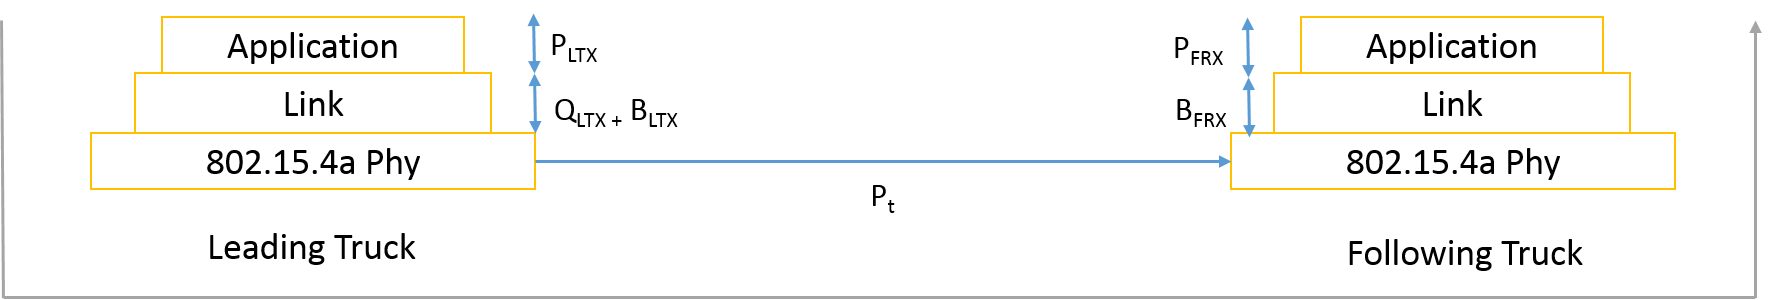
\includegraphics[width=1\textwidth]{figures/messageLatencyLeadingtoFollowing.png}
	\centering
	\caption{End to End latency when a message is transmitted from leading truck to the following truck}
	\label{fig:messageLatencyLeadingtoFollowing}    
\end{figure}
\begin{figure}[h!]
	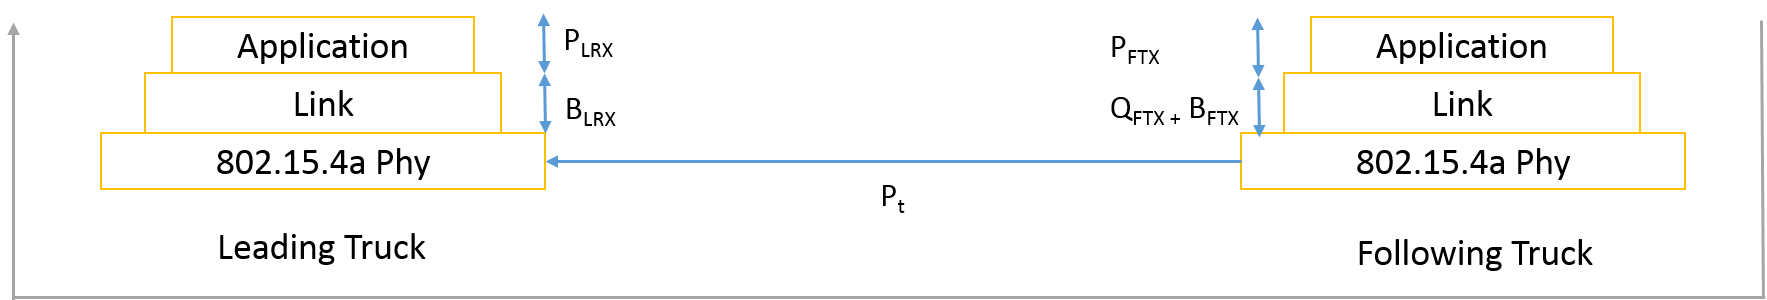
\includegraphics[width=1\textwidth]{figures/messageLatencyFollowingtoLeading.png}
	\centering
	\caption{End to End latency when a message is transmitted from following truck to the leading truck}
	\label{fig:messageLatencyFollowingtoLeading}    
\end{figure}

\subsection{End-to-End Latency/Message Latency}
The end-to-end latency/Message Latency is the time taken for a message to travel from the application layer of the leading truck to the application layer of the following truck or vice versa. We define the following variables:

    \begin{itemize}
    \item Processing time at the leading truck when transmitting a message, \emph{$P_{LTX}$}: In case of a message sent from the leading truck to the following truck,the  time taken to split a message into several packets and push it to the link layer of the leading truck.
    
    \item Processing time at the leading truck when receiving a packet, \emph{$P_{LRX}$}: In the case of a message sent from the following truck to the leading truck, the time taken for the received message to be completely processed by the application layer of the leading truck after the reception interrupt.
    
    \item Queuing time at the leading truck when transmitting a packet, \emph{$Q_{LTX} $}: When packets of a message are transmitted from the leading truck to the following truck, the time spent between transmission of each packet in the link layer of the leading truck.
    
    \item Queuing time at the following truck when transmitting a packet, \emph{$Q_{FTX} $}: When packets of a message are transmitted from the following truck to the leading truck, the time spent between transmissions of each packet in the link layer of the following truck.
    
    \item Processing time at the following truck when transmitting a message, \emph{$P_{FTX}$}:
    In the case of a message sent from the following truck to leading truck, time taken to split a message into several packets and push it to the link layer of the leading truck.
    
    \item Processing time at the following truck when receiving a packet, \emph{$P_{FRX}$}: In the case of a message sent from leading truck to the following truck, the time taken for the received message to be completely processed by the application layer of the following truck after the reception interrupt.
\end{itemize}

As shown in Figure \ref{fig:messageLatencyLeadingtoFollowing} and Figure \ref{fig:messageLatencyFollowingtoLeading}, the end-to-end/message latency for the leading truck transmitting a message and the following truck transmitting a message can be calculated using the Equation \ref{eq: messageLatencyLeading} and \ref{eq: messageLatencyFollowing} respectively wherein No\_of\_packets\_per\_message indicates the number of packets to be transmitted in a message. 
\begin{equation}
Message\_Latency_{LTX} = P_{LTX} + Q_{LTX} + No\_of\_packets\_per\_message * (B_{LTX}  +  P_{t} +  B_{FRX}) + P_{FRX}
\label{eq: messageLatencyLeading}
\end{equation}
\begin{equation}
Message\_Latency_{FTX} = P_{FTX} + Q_{FTX} + No\_of\_packets\_per\_message * (B_{FTX}  +  P_{t} +  B_{LRX}) + P_{LRX}
\label{eq: messageLatencyFollowing}
\end{equation}

\subsection{Reliable and Unreliable link}
We consider the links with MER less than 1\% as a reliable link because we are speaking about a secondary independent channel, wherein a loss of ten message for every thousand messages is acceptable for platooning.

\section{Measurement Goals}
To answer each of our research questions introduced in Section 1.4, we design a set of measurement goals corresponding to each question.

\subsection{Research Question RQ\_01}
What is the impact on the performance (Packet Error Ratio, Message Error Ratio, message latency, packet latency) of UWB in the presence of WiFi-p and vice-versa?

\subsubsection{Measurement Goal MG\_Interference}
In the measurement goal MG\_Interference, we investigate the performance of the UWB link in the presence of WiFi-p and vice versa based on link quality metrics PER, MER, message latency, and packet latency. Besides, we investigate the effect of Channel, Preamble Length, PRF (Pulse Repetition Frequency), Standard SFD, Non-standard SFD, Smart Power enablement, Preamble code on the performance of the UWB link in the presence of interference.

\subsubsection{Measurement Goal MG\_Distance\_Between\_Transceivers}
In the measurement goal MG\_Distance\_Between\_Transceivers, we study the influence of distance between UWB transceiver and WiFi-p transceiver on the links based on link quality metrics.


\subsubsection{Measurement Goal MG\_Worst\_Case\_Interference}
In the measurement goal MG\_Worst\_Case\_Interference, we investigate the performance of UWB link in the presence of WiFi-p and vice versa, by maximizing the time domain overlap of transmission instants, based on link quality metrics.

\subsection{Research Question RQ\_02}
Sensitivity analysis of performance under various conditions:

\subsubsection{Measurement Goal MG\_Speed\_Or\_Acceleration\_Difference}
In the measurement goal MG\_Speed\_Or\_Acceleration\_Difference, we investigate the performance of UWB link in the presence of speed or acceleration difference, based on link quality metrics.

\subsubsection{Measurement Goal MG\_Nulls}
In the measurement goal MG\_Nulls, we investigate the performance of UWB link at a distance of 20-30 m, based on link quality metrics. A null could arise because of negative interference from different multipaths. If the Line Of Sight (LOS) signal and the multipath signal, arrive at the destination at the same instant of time, negative interference could lead to no signal being received resulting in a null.

\subsection{Research Question RQ\_03}
What is the ranging accuracy that can be achieved through UWB when the trucks are operating in platooning mode?

\subsubsection{Measurement Goal MG\_Ranging\_Accuracy}
In the measurement goal MG\_Ranging\_Accuracy, we investigate the static ranging accuracy that can be achieved through UWB based on the difference between calculated distance and actual distance. Besides, we also examine the effect of Standard SFD and Non-Standard SFD on ranging accuracy.

\subsection{Research Question RQ\_04}
Which is the best configuration of UWB for platooning application?

Analyzing all the results, we determine the best configuration of UWB for platooning application.

\section{Network Topology}
We use point to point topology (Figure: \ref{fig:NetworkTopology}), wherein we have two nodes, namely the leading truck and the following truck. We use point to point topology as we consider platooning between two trucks as the situation under test and the existing EcoTwin Platooning project (project collaboratively developed by NXP, DAF Trucks and TNO) operates on the same topology \cite{euTPC}.

Below we describe the functions of each component present in our network topology (shown in Figure: \ref{fig:NetworkTopology}):

\begin{itemize}
    \item \textbf{Leading Truck}: In the communication state, the Vehicle Following Message (VFM) is sent from the leading truck to the following truck every 40 milliseconds starting from the instant of 0 millisecond. Also, it receives the Platoon Status Message (PSM) from the following truck. The node is an LPCXpresso 4337 board with DecaWave DW1000 transceiver.
    \item \textbf{Following Truck}: In the communication state, the PSM is sent from the following truck to the leading truck every 40 milliseconds starting from the instant of 20 milliseconds. Also, it receives the VFM from the leading truck. The node is an LPCXpresso 4337 board with DecaWave DW1000 transceiver.
    \item \textbf{Laptop/PC}: Laptop/PC is used as the human interface to log the data exported by the leading truck via the serial interface. The leading truck is interfaced to a laptop/PC through a USB port.
\end{itemize}

\begin{figure}[h!]
    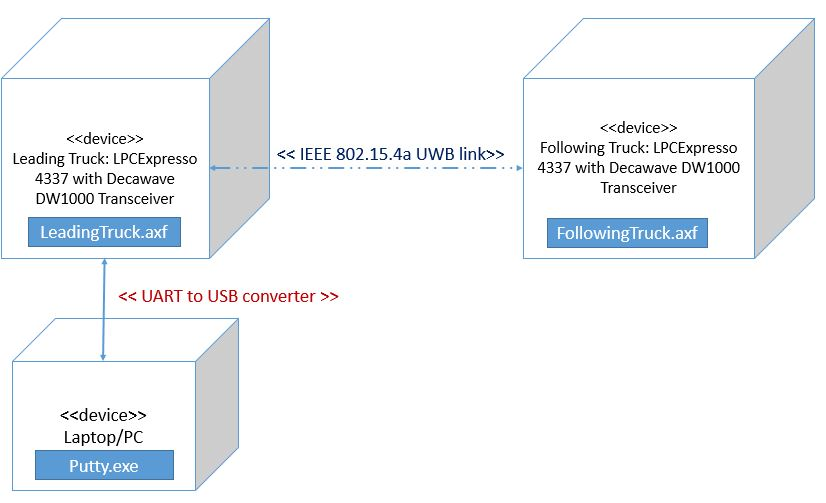
\includegraphics[width=1\textwidth]{figures/networkTopologyDeployment.JPG}
    \centering
    \caption{Point to Point topology deployment diagram}
    \label{fig:NetworkTopology}    
\end{figure}

\section{Data Communication Primitive}
We consider the data communication primitive to quantify the link characteristics in both directions: i. Uplink: leading truck to the following truck, and ii. Downlink: following truck to the leading truck.

    \textbf{Data Communication}: In the case of data communication state, VFM is sent from leading truck to the following truck every 40 milliseconds starting from the instant of 0 millisecond, PSM is sent from the following truck to leading truck every 40 milliseconds starting from the instant of 20 milliseconds. This communication primitive is designed to mimic the actual exchange of messages that occurs during platooning as shown in Figure \ref{fig:MessageExchangePlatooningApplication}.
    
    \begin{figure}[htbp]
        \begin{center}
            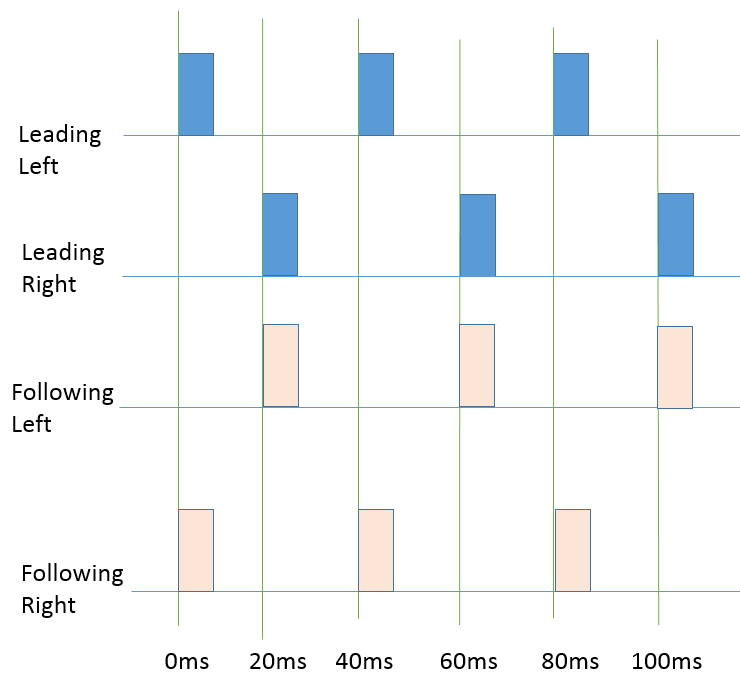
\includegraphics[width=0.8\textwidth]{figures/Picture6.png}
            \caption{Message Exchange in Platooning Application}
            \label{fig:MessageExchangePlatooningApplication}
        \end{center}
    \end{figure}

\section{Measurement Plan}
The measurement goals defined in Section 4.2 necessitate the need for varying different parameters such as packets per message, channels, PRF, preamble lengths, preamble codes, Standard or non-standard SFD, Smart Power enablement, distance, speed or acceleration, etc. to study their influence on the link quality. We design three measurement plans, to explore these measurement goals by sweeping a parameter over a range of values while keeping the other parameters constant. We use the measurement plan as a tool to perform experiments with/without vehicles and on the table top. Below we describe the measurement plans in detail.

\subsection{Measurement Plan MP\_Interference}
In measurement plan MP\_Interference, we investigate the performance of UWB in the presence of WiFi-p and vice versa based on link quality metrics. This measurement plan helps us to study measurement goals MG\_Interference, MG\_Distance\_Between\_Transceivers, and MG\_Worst\_Case\_Interference.

To introduce WiFi-p signals, we use equipment from Cohda wireless. Python scripts are used to monitor the sent and received messages. We operate WiFi-p in channel 184 corresponding to 5.920 GHz so that we get closest to channel 7 of UWB.

UWB transceivers are placed at an appropriate distance (0cm and 80cm) to the WiFi-p antennas, and we sweep several parameters as shown in Table \ref{configurationsMPInterference}. UWB transceiver - leading truck transmits every 40 ms starting at the 0 ms instant, and the UWB transceiver - following truck transmits every 40 ms starting at the 20 ms instant. We run a total of 44 configurations (\ref{app:ConfigurationsforMeasurementPlanMPInterference}) in this measurement plan varying several parameters as indicated in the Table \ref{configurationsMPInterference}.
% Please add the following required packages to your document preamble:
% \usepackage{graphicx}
\begin{table}[]
    \centering
    \caption{Configurations for measurement plan MP\_Interference}
    \label{configurationsMPInterference}
    \resizebox{\textwidth}{!}{%
        \begin{tabular}{|l|l|}
            \hline
            \textbf{Sweep Parameter}                            & \textbf{Value}                                \\ \hline
            Channels                                            & Channel 1, Channel 3, Channel 5 and Channel 7 \\ \hline
            PRF                                                 & 16Mhz and 64 MHz                              \\ \hline
            Data Rate                                           & 6.8 Mbps                                      \\ \hline
            Preamble Lengths                                    & 256, 128 and 64                               \\ \hline
            SFD                                                 & Standard or Non-Standard SFD                  \\ \hline
            Distance between WiFi-p antenna and UWB transceiver & 80 cm and 0 cm                                \\ \hline
            Smart Power Enablement                              & With and Without Smart Power Enablement       \\ \hline
            Preamble Code                                       & According to the Channel                      \\ \hline
        \end{tabular}%
    }
    
\end{table}

We conduct this measurement plan keeping the distance between UWB transceivers and WiFi-p Antenna at 80 cm and 0 cm to evaluate measurement goal MG\_Distance\_Between\_Transceivers. To assess MG\_Worst\_Case\_Interference, we transmit as quickly as possible (one message every 8 ms) from the UWB transceiver-leading truck and receive them at the UWB transceiver-following truck without adhering to the 40 ms constraint, so that we increase the time domain overlap between WiFi-p transmission and UWB transmission. 

\subsection{Measurement Plan MP\_Speed\_Or\_Acceleration\_Difference}
In measurement plan MP\_Speed\_Or\_Acceleration\_Difference, we mount the UWB transceivers on the mirrors of two cars. We make static measurements, following which we move one of the cars at 5-15 Km/hr to determine the influence of speed or acceleration difference on the performance of UWB link based on the link quality metrics. In this measurement plan, we vary parameters according to Table \ref{table:configurationsformeasurementplanMPSpeedDifference}. To overcome the major drawback of short range when using 6.8 Mbps data rate, we make use of 110 Kbps as the data rate in this measurement plan. This measurement plan helps us to study the measurement goals MG\_Nulls and MG\_Speed\_Or\_Acceleration\_Difference. 

% Please add the following required packages to your document preamble:
% \usepackage{graphicx}
\begin{table}[]
    \centering
    \caption{Configurations for measurement plan MP\_Speed\_Or\_Acceleration\_Difference}
    \label{table:configurationsformeasurementplanMPSpeedDifference}
    \begin{tabular}{|l|l|}
        \hline
        \textbf{Sweep Parameter} & \textbf{Value}               \\ \hline
        Channel                  & Channel 1                    \\ \hline
        PRF                      & 64 MHz                       \\ \hline
        Data Rate                & 110 Kbps                     \\ \hline
        Preamble Lengths         & 2048, 4096                   \\ \hline
        SFD                      & Standard or Non-Standard SFD \\ \hline
        Preamble Code            & According to the Channel     \\ \hline
    \end{tabular}
\end{table}


\subsection{Measurement Plan MP\_Distance}
In measurement plan MP\_Distance, we investigate the influence of distance on UWB link, based on the link quality metrics. Here, we keep the UWB transceivers at various distances and measure the link quality. In this measurement plan, we vary parameters according to the Table \ref{tab:configurationsforMPDistance}. This measurement plan helps us to study the measurement goals MG\_Ranging\_Accuracy and MG\_Nulls. We also determine the effect of antenna position on the link quality.

\begin{table}[]
    \centering
    \caption{Configurations for measurement plan MP\_Distance}
    \label{tab:configurationsforMPDistance}
    \begin{tabular}{|l|l|}
        \hline
        \textbf{Sweep Parameter} & \textbf{Value}                               \\ \hline
        Channel                  & Channel 1, Channel 4                         \\ \hline
        PRF                      & 16 MHz, 64 MHz                               \\ \hline
        Smart Power              & Enabled or Not Enabled                       \\ \hline
        Data Rate                & 110 Kbps, 850 Kbps, 6.8 Mbps                 \\ \hline
        Preamble Lengths         & 2048, 4096, 1024, 256                        \\ \hline
        SFD                      & Standard or Non-Standard SFD                 \\ \hline
        Preamble Code            & According to the Channel                     \\ \hline
        Antenna Position         & 0, 45, 90, 135, 180, 225, 270, 315 (degrees) \\ \hline
        Distance                 & 10, 15, 20, 25, 30, 35, 40, 45, 50 (meters)  \\ \hline
    \end{tabular}
\end{table}
\section{Test Platform Requirements}

The test platform implements the necessary functionalities to execute the measurement plans discussed in Section 4.5. Based on our measurement plans and measurement goals defined in the previous Sections, we develop the following set of requirements for our test platform.

\begin{enumerate}
    \item It must support point to point topology with one transceiver-leading truck and another transceiver-following truck. 
    \item It must implement data communication workload and transmit/receive according to the 40 ms schedule.
    \item It must enable us to vary parameters such as packets per message, channels, PRF, preamble lengths, preamble codes, Standard or non-standard SFD and Smart Power enablement.
    \item It must capture physical layer metrics such as Channel Impulse Response Power (CIRP), Preamble Accumulation Count (PAC), accurate time stamps for ranging, and sequence numbers of the test payload, at both transceivers.
    \item It must enable the following truck to store the logging information and communicate this information to the leading truck.
    \item It must allow the transceivers to send the logging information and print the log via the serial interface connection to the laptop/PC.
    \item It should run autonomously without human intervention and execute all possible test combinations of parameters based on the selected measurement plan so that the manual effort required for the same can be significantly reduced.
\end{enumerate}

\section{Post Processing Requirements}
The task of the post-processing scripts is to parse and extract useful information from the logs created during the experiments.

For the post processing we have the following requirements:
\begin{enumerate}
    \item It must be able to process logs resulting from a full night test.
    \item It should parse the log files and store the data appropriately so that desired kind of graphs such as PER vs. Channel, MER vs. Channel, MER vs. Distance, Measured Distance vs. Calculated Distance, etc. can be created.
\end{enumerate}
\clearemptydoublepage

\chapter{Test Platform Implementation}\label{chapter:testPlatformImplementation}
\nomenclature[A]{CRC}{Cyclic Redundancy Check}
\nomenclature[A]{TOF}{Time of Flight}
\nomenclature[A]{DS-TWR}{Double Sided Two Way Ranging}
\nomenclature[A]{API}{Application Programming Interface}
\nomenclature[A]{SPI}{Serial Peripheral Interface Bus}
\nomenclature[A]{IRQ}{Interrupt Request}
\nomenclature[A]{GPIO}{General Purpose Input/Output Pin}
In this chapter, we describe in detail the design (Section 5.1), key design choices (Section 5.2), and the implementation details (Section 5.3) of the Test Platform for evaluation and analysis of UWB (TP-UWB).

\section{Test Platform Design}
The test platform as shown in Figure \ref{fig:phasesOfTestPlatform} consists of five phases:
\begin{figure}[h!]
	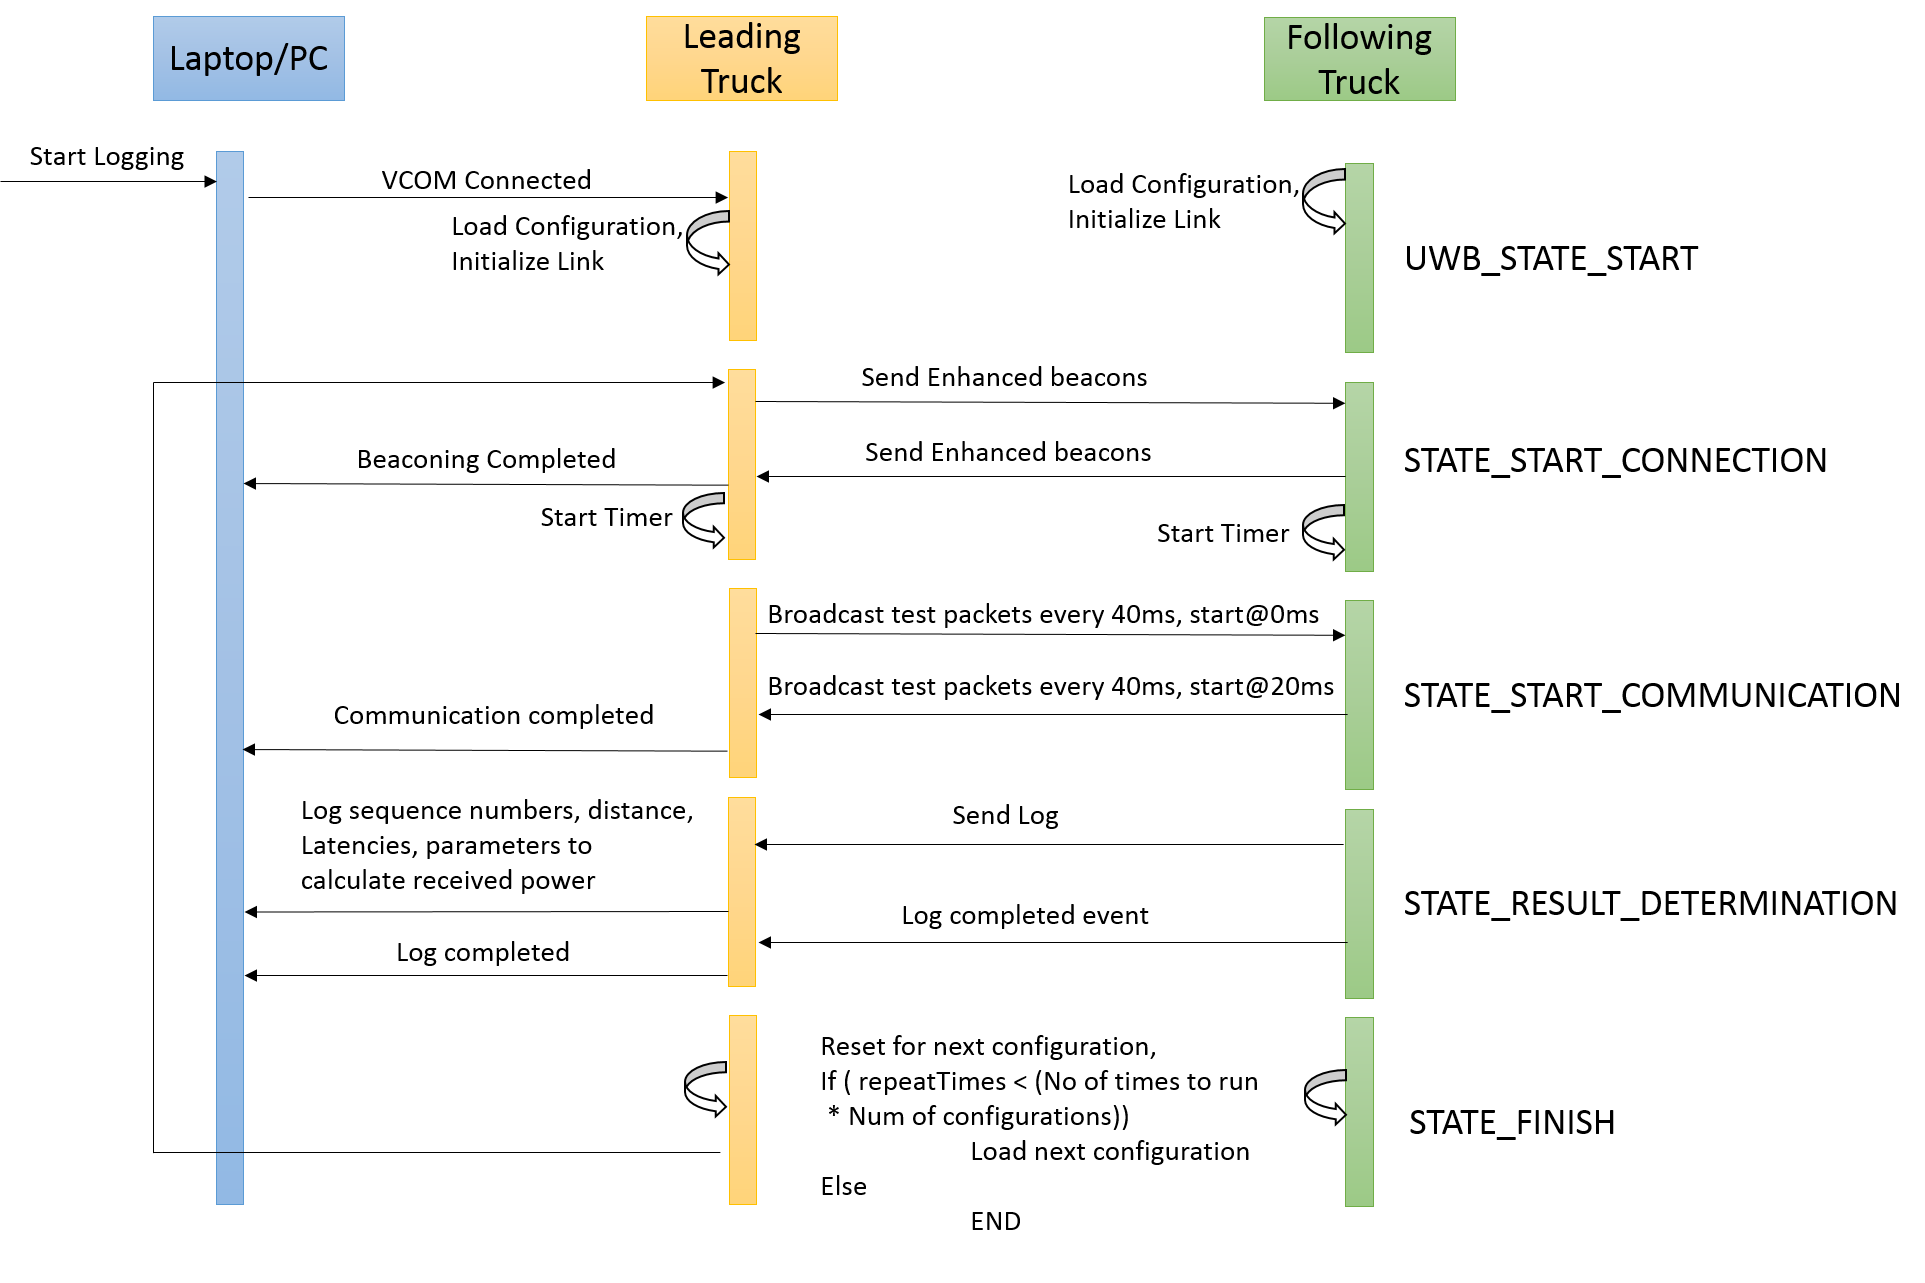
\includegraphics[width=1\textwidth,keepaspectratio]{figures/PhasesofTestPlatform}
	\centering
	\caption{Phases of test platform}
	\label{fig:phasesOfTestPlatform}    
\end{figure}
\begin{enumerate}
    \item \textbf{UWB\_STATE\_START}: In this phase, the leading truck will be waiting for the VCOM connected event from the laptop/PC to start execution. Once it receives this event, the first configuration is loaded, and the link is initialized. The following truck does not wait for the VCOM connected event and starts execution on power-up wherein the first configuration is loaded, and the link is initialized. In link initialization, we set the MAC address of the node, configure event counters, set the receiver to infinite timeout, set preamble detect to infinite timeout, enable frame filtering only to accept acknowledgment, data and beacon frames destined to that particular node. Also, we enable interrupts for frame sent, frame received with good CRC, receiver PHY header error, receiver CRC error, receiver sync loss error, frame wait timeout, preamble detect timeout, SFD timeout and frame rejected. Moreover, we set the pointer to the TX callback function that gets executed after the transfer of a packet and set the pointer to the RX callback function that gets executed after the reception of a packet.
    
    \item \textbf{STATE\_START\_CONNECTION}: In this phase, the following truck will be waiting infinitely for the first beacon. The leading truck will transmit a beacon every 10 ms starting at 0 ms instant and wait for the reception of a beacon from the following truck until the next transmission. In each beacon, it transmits the remaining number of beacons it requires to go to next state. Similarly, the following truck sends a beacon (indicating the required remaining number of beacons) every 5 ms and waits for the reception of a beacon from the leading truck until next transmission. Once a defined number of beacons are received sequentially, the leading truck and the following truck go into the next state respectively.  
    
    \item \textbf{STATE\_START\_COMMUNICATION}: In this phase, the leading truck broadcasts test messages every 40 ms starting at 0 ms time instant and the following truck broadcasts text messages every 40 ms starting at 20 ms time instant. We synchronize on the reception of the first packet from the leading truck to the following truck. The following truck stores the log information (sequence numbers, message latency, packet latency, distance and values for calculation of received power level) of the test packet received from the leading truck.
    
    \item \textbf{STATE\_RESULT\_DETERMINATION}: In this phase, the following truck sends the stored log information of the received test packets to the leading truck. The leading truck on receiving this log information, sends it serially to the laptop, along with its log information of the received test packets from the following truck.
    
    \item \textbf{STATE\_FINISH}: During this phase, we reset for execution of the next configuration, if (repeatTimes \textless (No of times to run * Number of configurations)), we load the next configuration and go to the STATE\_START\_CONNECTION phase, else the test is stopped.
    
\end{enumerate}

%Phases of Test Platform
%Ranging
%State Machine of Leading Truck
%State Machine of Following Truck
%For each phase, process flow
%What happens during Transmission
%What happens during Reception etc...


\section{Important Design Choices}
Below we list the key design choices of the test platform:
\begin{enumerate}
    \item Suitable ranging method: We have three different ways, the pros and cons of each method are provided in Table \ref{table:DesignChoiceRanging}. We choose Double Sided Two Way Ranging (DS-TWR) as the method for implementing ranging attributed to the facts that the number of packets required for ranging is small when the application is considered for a large number of following trucks, reply times can be asymmetric, and error in calculated TOF is minimized. Also, the processor on LPCXpresso4337 can easily handle multiplication and division operations in a short duration of time.
   \begin{table}
       \centering
       \begin{longtable}{@{\extracolsep{\fill}}| p{2.55cm}  | p{4.8cm} | p{5cm} | p{5cm} |@{}}
           \hline
           \centering {\textbf{Design Choice}} &\centering {\textbf{Pros}   }                                                                                                                                                                                                   & \centering {\textbf{Cons}}                                                                                                                                                                                                                                                                                                                                                                                                                                                                                                     \\ \vspace{-3mm}\hline
           Single Sided Two way Ranging  & \vspace{-7mm} \begin{itemize}[leftmargin=*]
               \item Only one message exchange required which saves time \& power (within approx. 40 ms + delta time, the ranging value can be determined).\end{itemize}   & \vspace{-7mm} \begin{itemize}[leftmargin=*]
               \item Time of Flight (TOF) estimate error increases as Treply increases (turn around time) and as clock offset increases. 
               \item If tight tolerance clocks are used, Treply is short \& communication range is relatively short then it might be worthy of examination.   \end{itemize}\\                                                                                                                                                                                        \hline
           Double Sided Two way Ranging          &  \vspace{-7mm} \begin{itemize}[leftmargin=*] \item Reply times need not be the same. \item Error in calculated TOF is minimized. \item In case of platooning, the number of packets required to determine the range = N+2 (N=Number of following trucks). \end{itemize}& \vspace{-7mm} \begin{itemize}[leftmargin=*] \item Requires multiplication and division operations. \item Requires 4 messages to determine the range \item Within approx. 80 ms + delta time, the ranging value can be determined.  \end{itemize}                                                                                                      \\ \hline
           Symmetric Double-Sided Two way Ranging  & \vspace{-7mm} \begin{itemize}[leftmargin=*] \item Requires only simple math operations to derive a result. \end{itemize}                                                                                                                                                                                & \vspace{-7mm} \begin{itemize}[leftmargin=*] \item Does not seem suitable for platooning when the number of trucks in the platoon is increased as the number of packets required for ranging = 3N (N= Number of following trucks). \item Reply times must be the same - difficult to achieve. \item Error induced is proportional to difference between the reply times. \item The ranging exchange is longer than necessary because all reply times must be as long as the longest reply time. \item Increase in latency. \end{itemize} \\ \hline
           \caption{Design Choice - Ranging}
           \label{table:DesignChoiceRanging}
       \end{longtable}
   \end{table}
    \item Compliance to standards or non-compliance to standards: This question arises due to the additional 39 bytes (maximum value) of MAC header for each packet. The pros and cons of these two options are indicated in the Table \ref{table:ComplianceStandardsvsNonCompliance}. We choose to comply to the IEEE 802.15.4 standard so as to support interoperability, and hence break messages (\textgreater 127 bytes) into several 127 byte packets. 
    % Please add the following required packages to your document preamble:
    % \usepackage{graphicx}
   % Please add the following required packages to your document preamble:
   % \usepackage{graphicx}
   \begin{table}
       \centering
       \begin{longtable}{| p{2.55cm}  | p{4.8cm} | p{5cm} | p{5cm} |}
           \hline
           \centering {\textbf{Design Choice}} &\centering {\textbf{Pros}   }                                                                                                                                                                          & \centering {\textbf{Cons}}                                                                                                                                                                                                                                                                                                                                                                                                                                                                                                                                                                                                                                                               \\ \vspace{-3mm}\hline
           Compliance to Standards     &  \vspace{-7mm} \begin{itemize}[leftmargin=*] \item Interoperability: Ability of devices to work together relies on products and services complying with standards. \item Reliability \& Safety: More dependable. \item Foundation for new features \item Business benefits: Market access, awareness, etc.\end{itemize} & 
           \vspace{-7mm} \begin{itemize}[leftmargin=*] \item Additional latency during communication. \item Increase in coding complexity as messages (\textgreater 127 bytes) need to be broken down into several 127 byte packets\end{itemize} \\ \hline
           Non Compliance to Standards & \vspace{-7mm} \begin{itemize}[leftmargin=*] \item Decrease in latency during communication. \item Decrease in coding complexity.\end{itemize}                                                                                                                                                                              & \vspace{-7mm} \begin{itemize}[leftmargin=*] \item Incompatibility with other equipment. \item Restricted to one manufacturer or supplier\end{itemize}                                                  \\ \hline
       \end{longtable}
       \caption{Compliance to Standards vs Non Compliance}
       \label{table:ComplianceStandardsvsNonCompliance}
   \end{table}
    
    \item Choice of data rate: The pros and cons for all the available three data rates are provided in the table \ref{table:prosconsdatarate}. We make use of all the three data rates in different measurement plans attributed to their respective advantages.
   % Please add the following required packages to your document preamble:
   % \usepackage{graphicx}
   \begin{table}
       \centering
       \begin{longtable}{| p{2.55cm}  | p{4.8cm} | p{5cm} | p{5cm} |}
           \hline
           \centering {\textbf{Data Rate Parameter} }& \centering {\textbf{Pros}     }                                                                                                                                                                                               & \centering {\textbf{Cons}      }                                                                                                          \\ \vspace{-3mm}\hline
           110 Kbps                     & \vspace{-7mm} \begin{itemize}[leftmargin=*] \item Range of signal increases. \item Ideal for better ranging results and high multipath environments.\end{itemize}                                                                       & \vspace{-7mm} \begin{itemize}[leftmargin=*] \item Very high latency (13.5424 ms). \end{itemize}                                                                                            \\ \hline
           850 Kbps                     & \vspace{-7mm} \begin{itemize}[leftmargin=*] \item Latency better than that of 110 kbps (2.2430 ms). \item Ranging accuracy better than that of 6.8 Mbps. \end{itemize}                                                                     & \vspace{-7mm} \begin{itemize}[leftmargin=*] \item Latency more than that of 6.8 Mbps. \item Ranging accuracy less than that of 110 Kbps.\end{itemize} \\ \hline
           6.8 Mbps                     & \vspace{-7mm} \begin{itemize}[leftmargin=*] \item Low latency (0.4404 ms). \item Data rate similar to that of 802.11p. \item Shortened Tx and Rx times, better battery \& appropriate for burst interference environments.\end{itemize} & \vspace{-7mm} \begin{itemize}[leftmargin=*] \item Ranging accuracy will be reduced, \item Range/distance reduces\end{itemize}                        \\ \hline
       \end{longtable}
       \caption{Pros/Cons - Data Rate}
       \label{table:prosconsdatarate}
   \end{table}
    
    \item Choice of Preamble Length and SFD or Non-standard SFD:  
    \begin{itemize}
        \item \textbf{Shorter preamble length}: Reduces transmission and reception time.
        \item \textbf{Longer preamble length}: Guarantees higher security, improves range and ranging accuracy.
        \item \textbf{Non-standard SFD sequence}: More robust than IEEE 802.15.4 standard, improved performance and improved ranging accuracy because of more accurate time stamps.
        \item \textbf{Standard SFD sequence}: If we use non-standard SFD, it will be impossible to inter-work with a device expecting a standard SFD sequence.
    \end{itemize}    
    From the above facts, instead of choosing a single preamble length or Standard SFD or non-standard SFD, we use them as a sweep parameter to determine the influence of these factors on the performance of UWB.   
    \item The test platform consists of two application binaries which will be flashed into the respective devices (leading truck and the following truck). One application implements the functions of the leading truck and will be flashed to the leading truck and other implements the functions of the following truck and will be flashed into the following truck.
    \item We send data communication packets from the leading truck to the following truck and vice-versa every 40 ms according to the typical platooning application requirement.
    \item We log the values onto the laptop/computer only at the end of configuration execution because printing the logs serially during communication causes deviation from the desired schedule when the COM port is busy. Hence we store the required values until the end of configuration execution.
    \item Limited by the logging information that can be stored in RAM, we send 250 messages when we have three or four packets per message and 500 messages when we have two or one packet per message.
    \item There exist state transitions in the leading truck and the following truck. We make use of the timeout mechanism in both leading truck and the following truck to come out of a phase if it does not receive within the maximum time window. For example, in the communication state, both nodes transmit messages at their respective time instants irrespective of whether a message is received or not and move into the next state as designed.
    \item We operate in two settings: reliable and test settings. We make use of 110 Kbps data rate in the reliable settings. We are in reliable settings during the STATE RESULT DETERMINATION. We use test settings during the STATE START COMMUNICATION. The test settings are based on the current test case.
    \item There are four types of messages exchanged between the nodes namely: MSG ID TEST DATA, MSG ID COMMUNICATION RESULT, ACK, BEACON in states STATE START COMMUNICATION, STATE RESULT DETERMINATION, STATE RESULT DETERMINATION, STATE START CONNECTION respectively.
    \item The following truck synchronizes on the first communication packet received in the STATE START COMMUNICATION. We do not use beacons to synchronize every message considering the additional packet that needs to be transmitted. The additional packet for every message plays a significant role considering the latency and LDC requirements of the system, and operation of the platooning application.
    
\end{enumerate}
\section{Architecture}
The system is designed to operate as a UWB subsystem in the platooning system as shown in Figure \ref{fig:integrationOfUWBToExistingSystem} wherein UWB acts as a secondary independent back up channel.
The software overview of TP\_UWB is shown in Figure \ref{fig:softwareOverview}. We use NXP LPCXpresso4337 development board, which has a dual-core: Cortex M4 and M0 MCU. The DW1000 UWB transceiver is connected to LPCXpresso4337. TP\_UWB software is organized as two files namely application and link. The link file makes use of DecaWave device Application Programming Interface (API) to interact with the transceiver. 'DW1000' file ports the DecaWave device API to the LPCXpresso4337. The interface between LPCXpresso4337 and DW1000 is through the DecaWave device API, which internally makes use of a Serial Peripheral Interface Bus (SPI), an Interrupt Request (IRQ) and a General Purpose Input/Output pin (GPIO).
\begin{figure}[h!]
	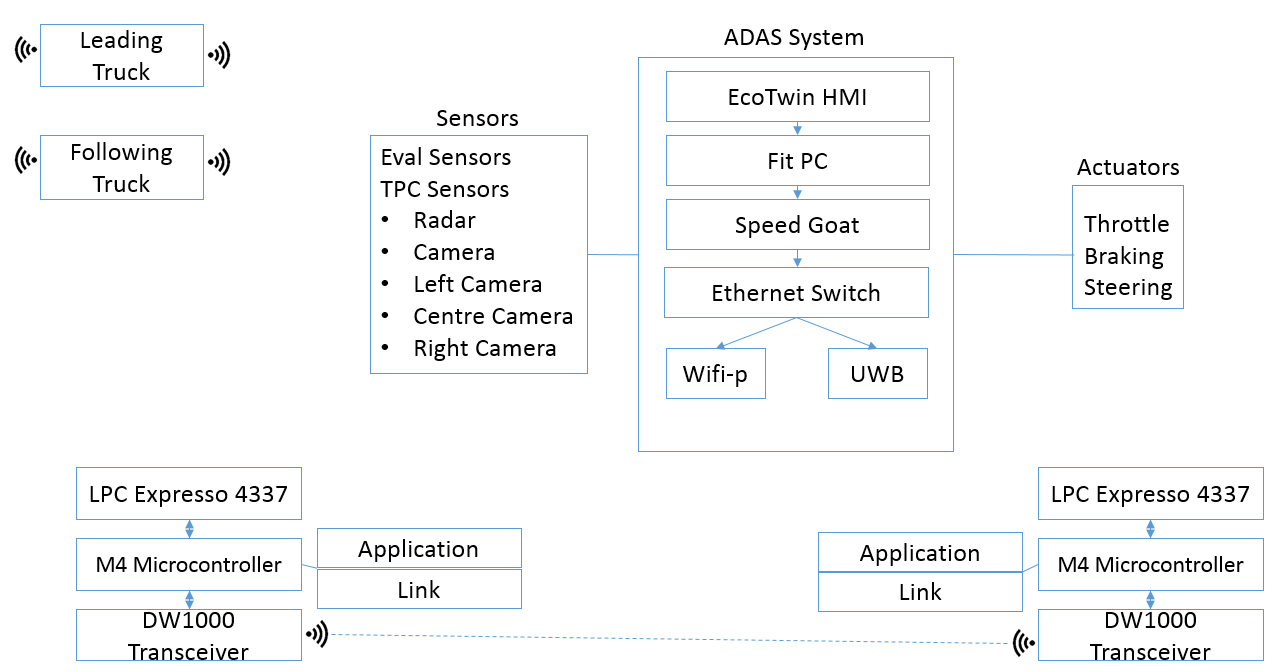
\includegraphics[width=1\textwidth]{figures/IntegrationOfUWBtoExistingSystem}
	\centering
	\caption{Wifi-p + UWB in platooning system}
	\label{fig:integrationOfUWBToExistingSystem}    
\end{figure}
\begin{figure}[h!]
    \includegraphics[width=3in]{figures/SoftwareOverview}
    \centering
    \caption{Software Overview}
    \label{fig:softwareOverview}    
\end{figure}

\section{Implementation}
Below we explain the set of actions executed in each state and the events which cause state transitions in detail.

\subsection{State Connection}
For this phase, several methods were tried. In the first method, the desired number of beacons were sent from the leading truck to the following truck, and the same number of desired beacons were sent from the following truck to the leading truck. In the latter case, the number of beacons received from the leading truck is sent in the beacons from the following truck to the leading truck. Finally, the number of beacons received from the following truck is sent in the beacons from leading to the following truck. The timeout for this phase was set to 300 ms and even on successful completion of all the above three transmissions and receptions, we wait for the elapse of this 300 ms. So that both the devices enter the next state at the same time. If the number of beacons received is more than the desired number, then the node goes to the next state, else repeat. This method did not work in all circumstances, in few special cases, the code went into infinite trials. Another method that was tried was to have 200 ms and 300 ms as respective timeout durations for leading truck and the following truck respectively. This method was also not effective.

Next method was to transmit a beacon every 10 ms from the leading truck to the following truck with the remaining number of beacons to be received to move to the next state and wait for reception of a beacon until its next transmission. Here, the following truck transmits a beacon every 5 ms to the leading truck with the remaining number of beacons to be received to move to the next state. The respective nodes were to receive a desired number of beacons to go to the next stage. This method of beaconing failed if the last beacon was received in the following truck but not in the leading truck.

The method that worked appropriately was to synchronize on the first packet that is received in the following truck from the leading truck in STATE\_COMMUNICATION. 

\subsection{State Communication}
The working of state communication phase is given in Figure \ref{fig:stateCommunication}. On entering this phase, we set a variable \emph{communicationMode} to 1 and on leaving this phase, we set it back to 0. This ensures that a part of the interrupt handler is executed only when executing in this particular phase. We set \emph{autorxreenable} to 1, so that in a case of an error during a reception, the receiver is re-enabled quickly. We set default antenna delay values for transmission and reception. 

In the case of the following truck, we set Timer2 to interrupt after 20 ms, Timer1 to interrupt every 40 ms and Timer 3 to tick every 1 $\mu$s. It is to be noted that we only set the three timers but do not enable them immediately. We enable reception for the first message. The following truck waits indefinitely for the first packet. On reception of the first packet, we enable Timer3 and Timer2. While waiting for the other packets of a message, if the Timer2 interrupt occurs then we go ahead and transmit the next message according to the schedule of every 40 ms with an offset of 20 ms from the leading truck. Even on the successful reception of the first message, we wait for Timer2 interrupt to occur. We enable Timer1, and if the messageCounter is less than or equal to \emph{NO\_OF\_MESSAGES}, then we transmit and enable reception. On the occurrence of every Timer1 interrupt, we enable Timer2 for reception timeout duration. Hence for the first instant when Timer1 is enabled, we define reception timeout for this instant using software defined timeout (Timer3). After successful/unsuccessful reception of this second message, we wait for the Timer1 interrupt to occur. It is to be noted that Timer2 is enabled in the interrupt handler of Timer1 interrupt, hence the occurrence of Timer1 interrupt indicates Timer2 is enabled for reception timeout duration. We transmit a message if messageCounter is less than or equal to \emph{NO\_OF\_MESSAGES} at this instant and enable the receiver until Timer2 interrupt. As a consequence of the successful/unsuccessful reception, we wait for Timer1 interrupt, transmit a message if messageCounter is less than or equal to \emph{NO\_OF\_MESSAGES}, and enable reception. This process continues until messageCounter is equal to the \emph{NO\_OF\_MESSAGES}.

In the case of the leading truck, we set Timer1 to interrupt every 40 ms, Timer3 to tick every 1 $\mu$s. On transmission of the first packet, we enable Timer3 and Timer1. Similar to the case of the following truck, on the occurrence of every Timer1 interrupt, we enable Timer2 for the reception timeout duration. Hence for the first instant when Timer1 is enabled, we define reception timeout for this instant using software defined timeout (Timer3). After successful/unsuccessful reception of this message, we wait for the Timer1 interrupt to occur. This process now continues very similar to that of the following truck indicated above. The test data structure data type is shown in Listing \ref{lst:testDataStructureDefinition}.

\begin{lstlisting}[caption={Test data structure definition}, label={lst:testDataStructureDefinition}, language=C]
typedef struct {
uint8 type;
uint8 timeStamp[4];
uint8 rangingMessage[32];
uint8 transferPayload[PAYLOAD_SIZE_CAN_TRANSMIT];
} msg_app_test_data;
\end{lstlisting}
\begin{figure}[h!]
    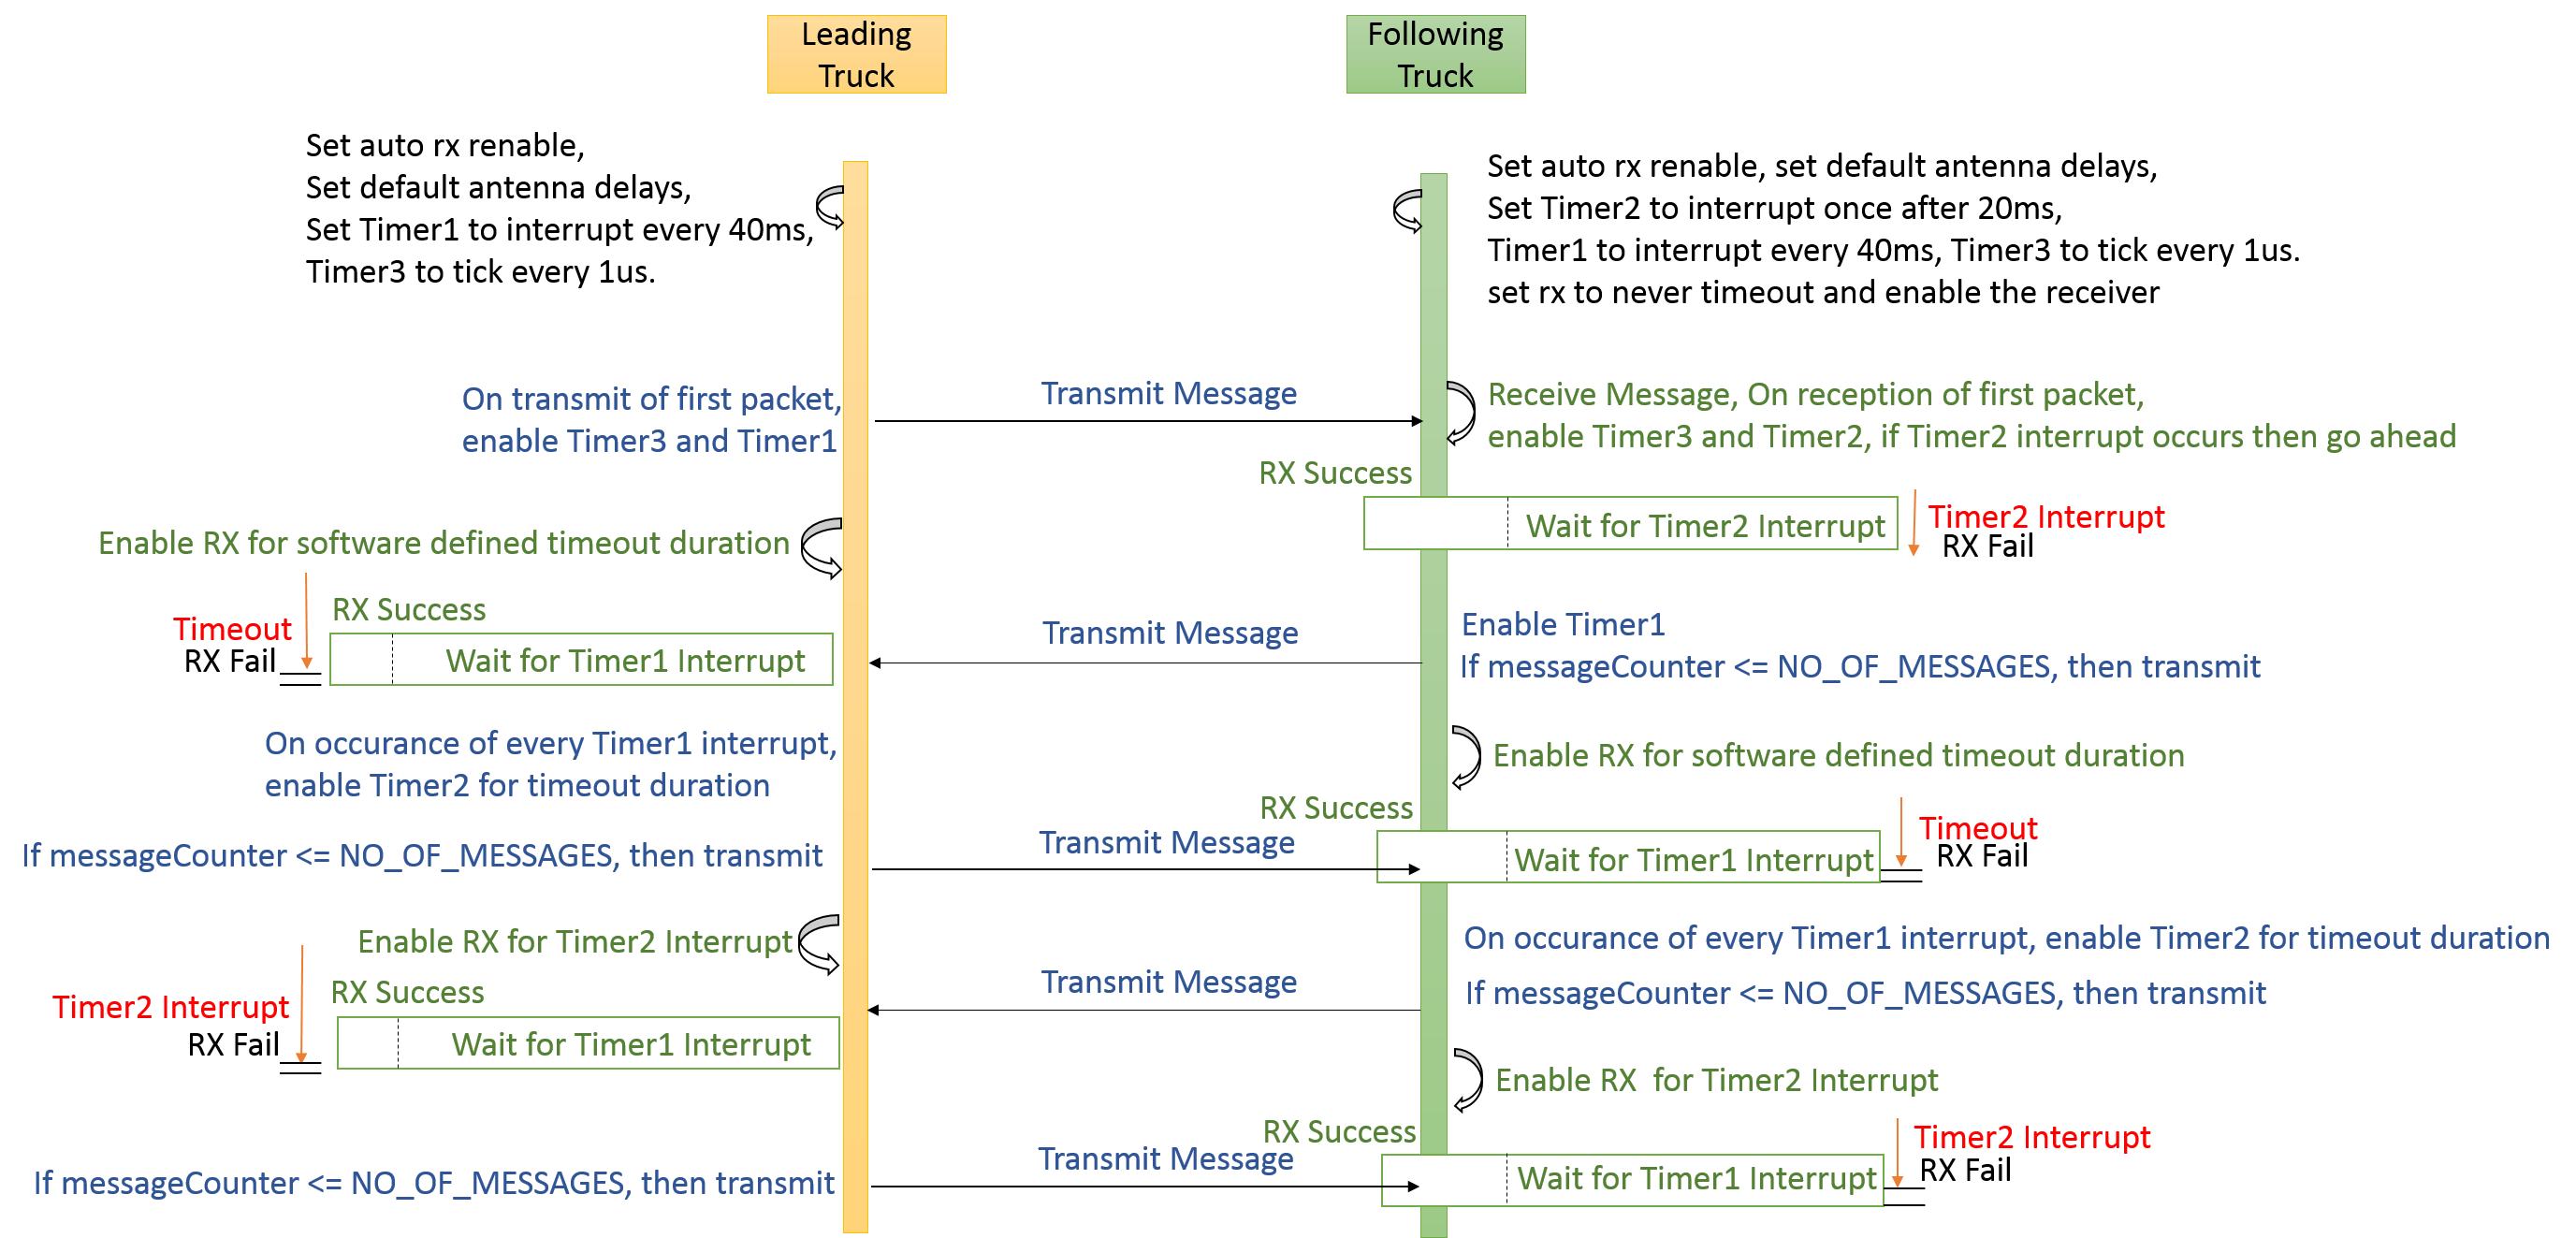
\includegraphics[width=1\textwidth]{figures/StateCommunicationPhase}
    \centering
    \caption{Process flow in State Communication}
    \label{fig:stateCommunication}    
\end{figure}
\begin{figure}[h!]
	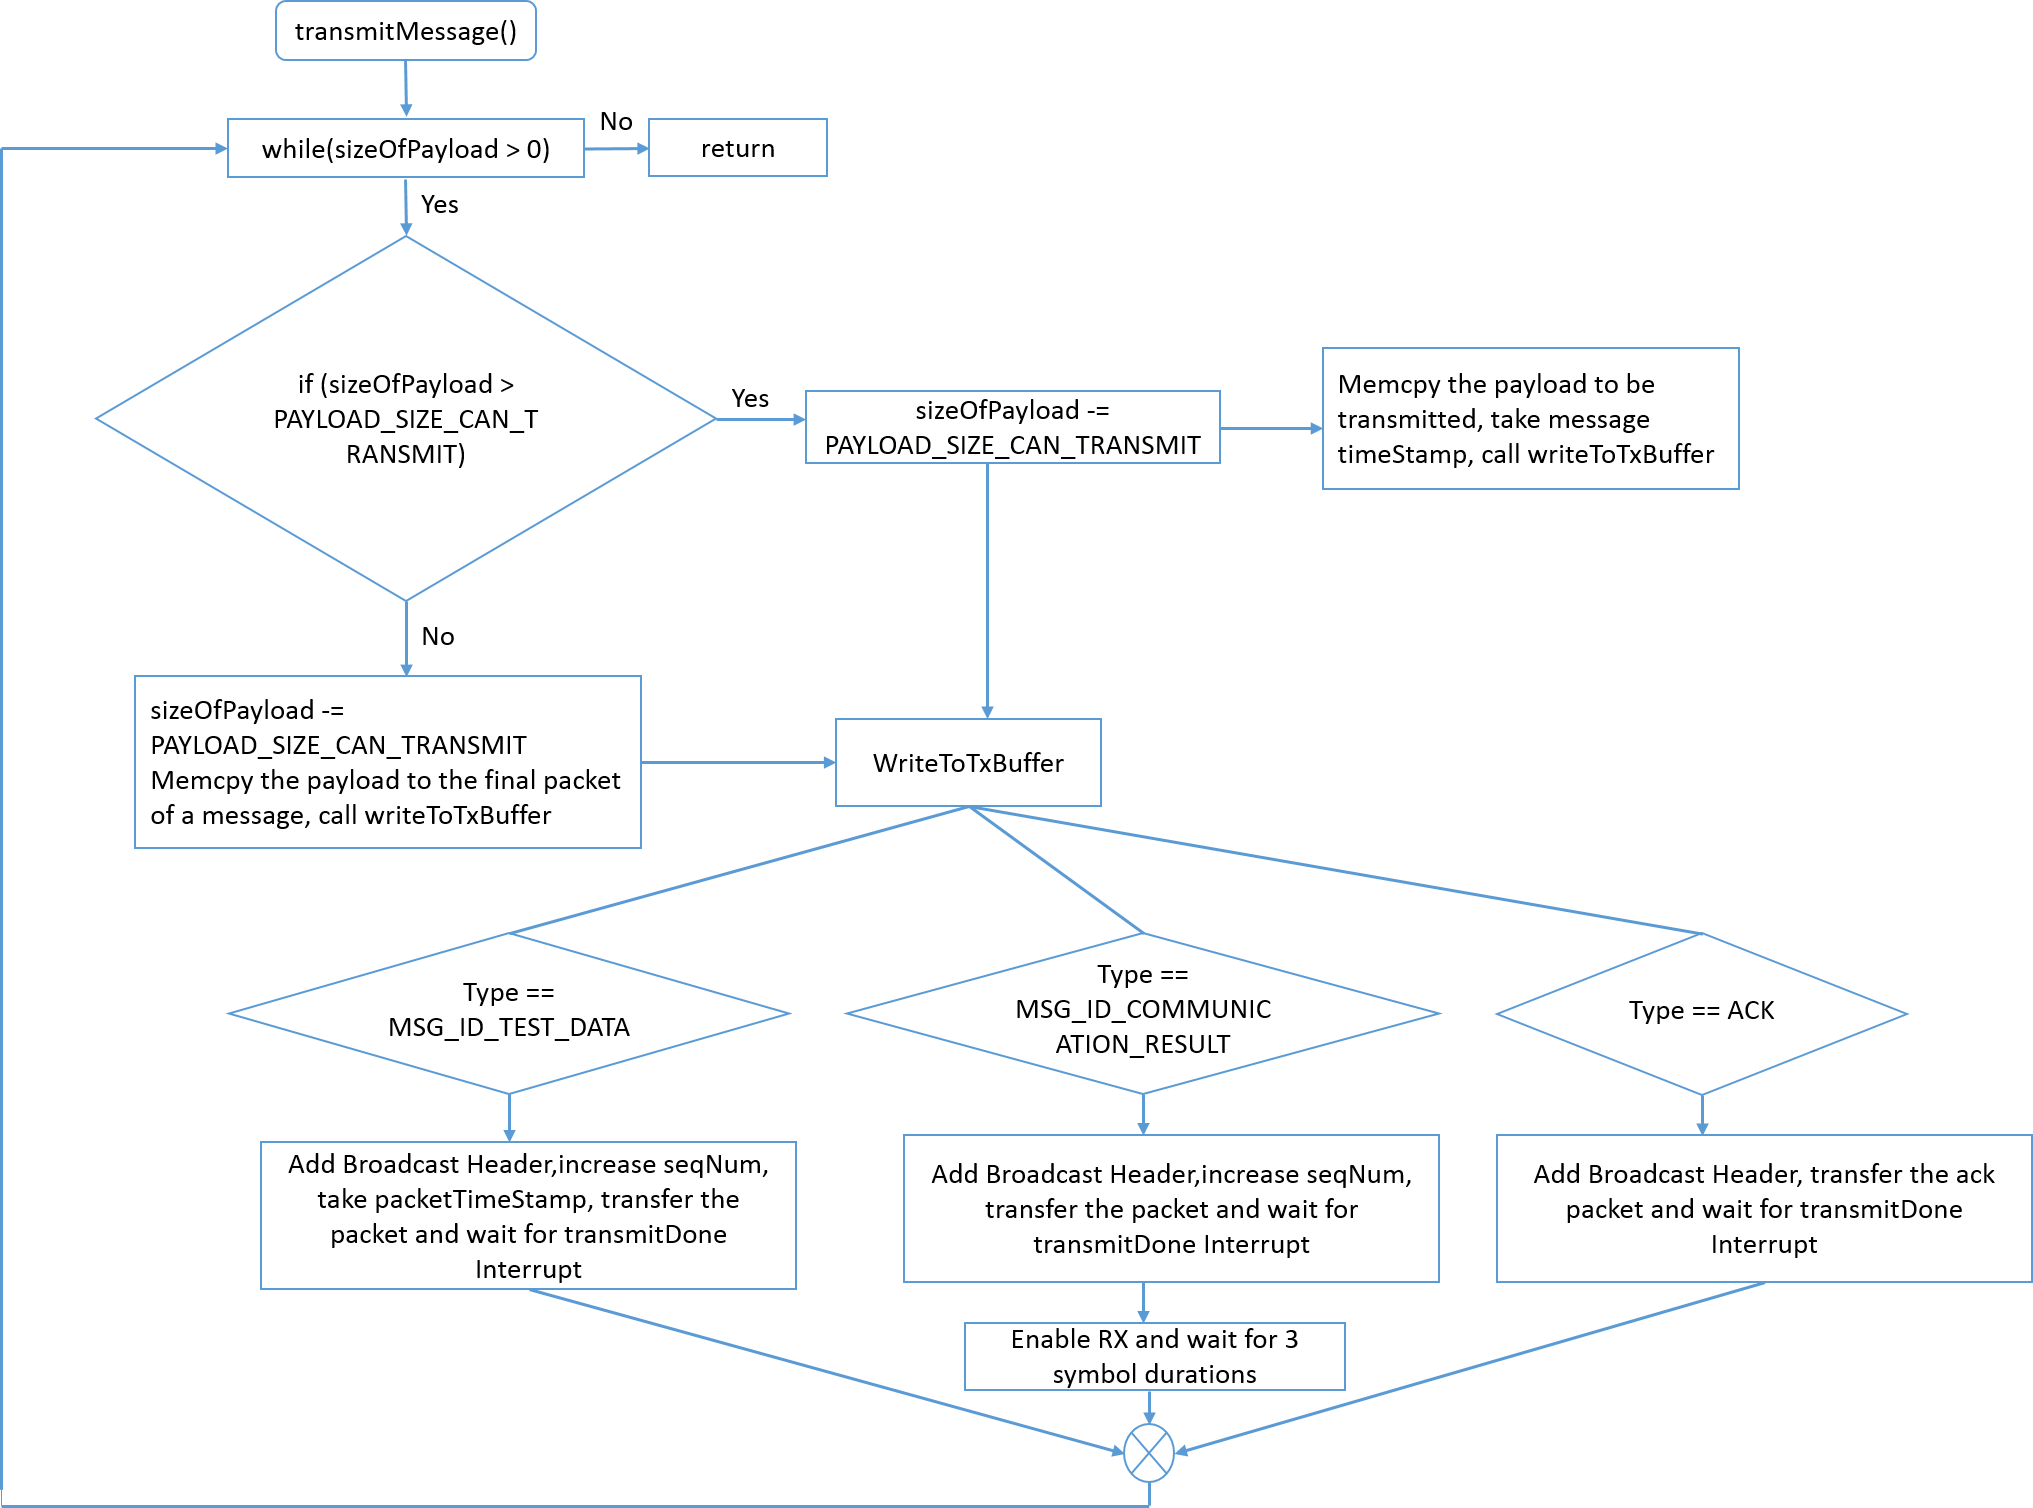
\includegraphics[width=1\textwidth]{figures/transmitMessage}
	\centering
	\caption{Process of transmission of a message}
	\label{fig:transmitMessage}    
\end{figure}
\begin{figure}[h!]
	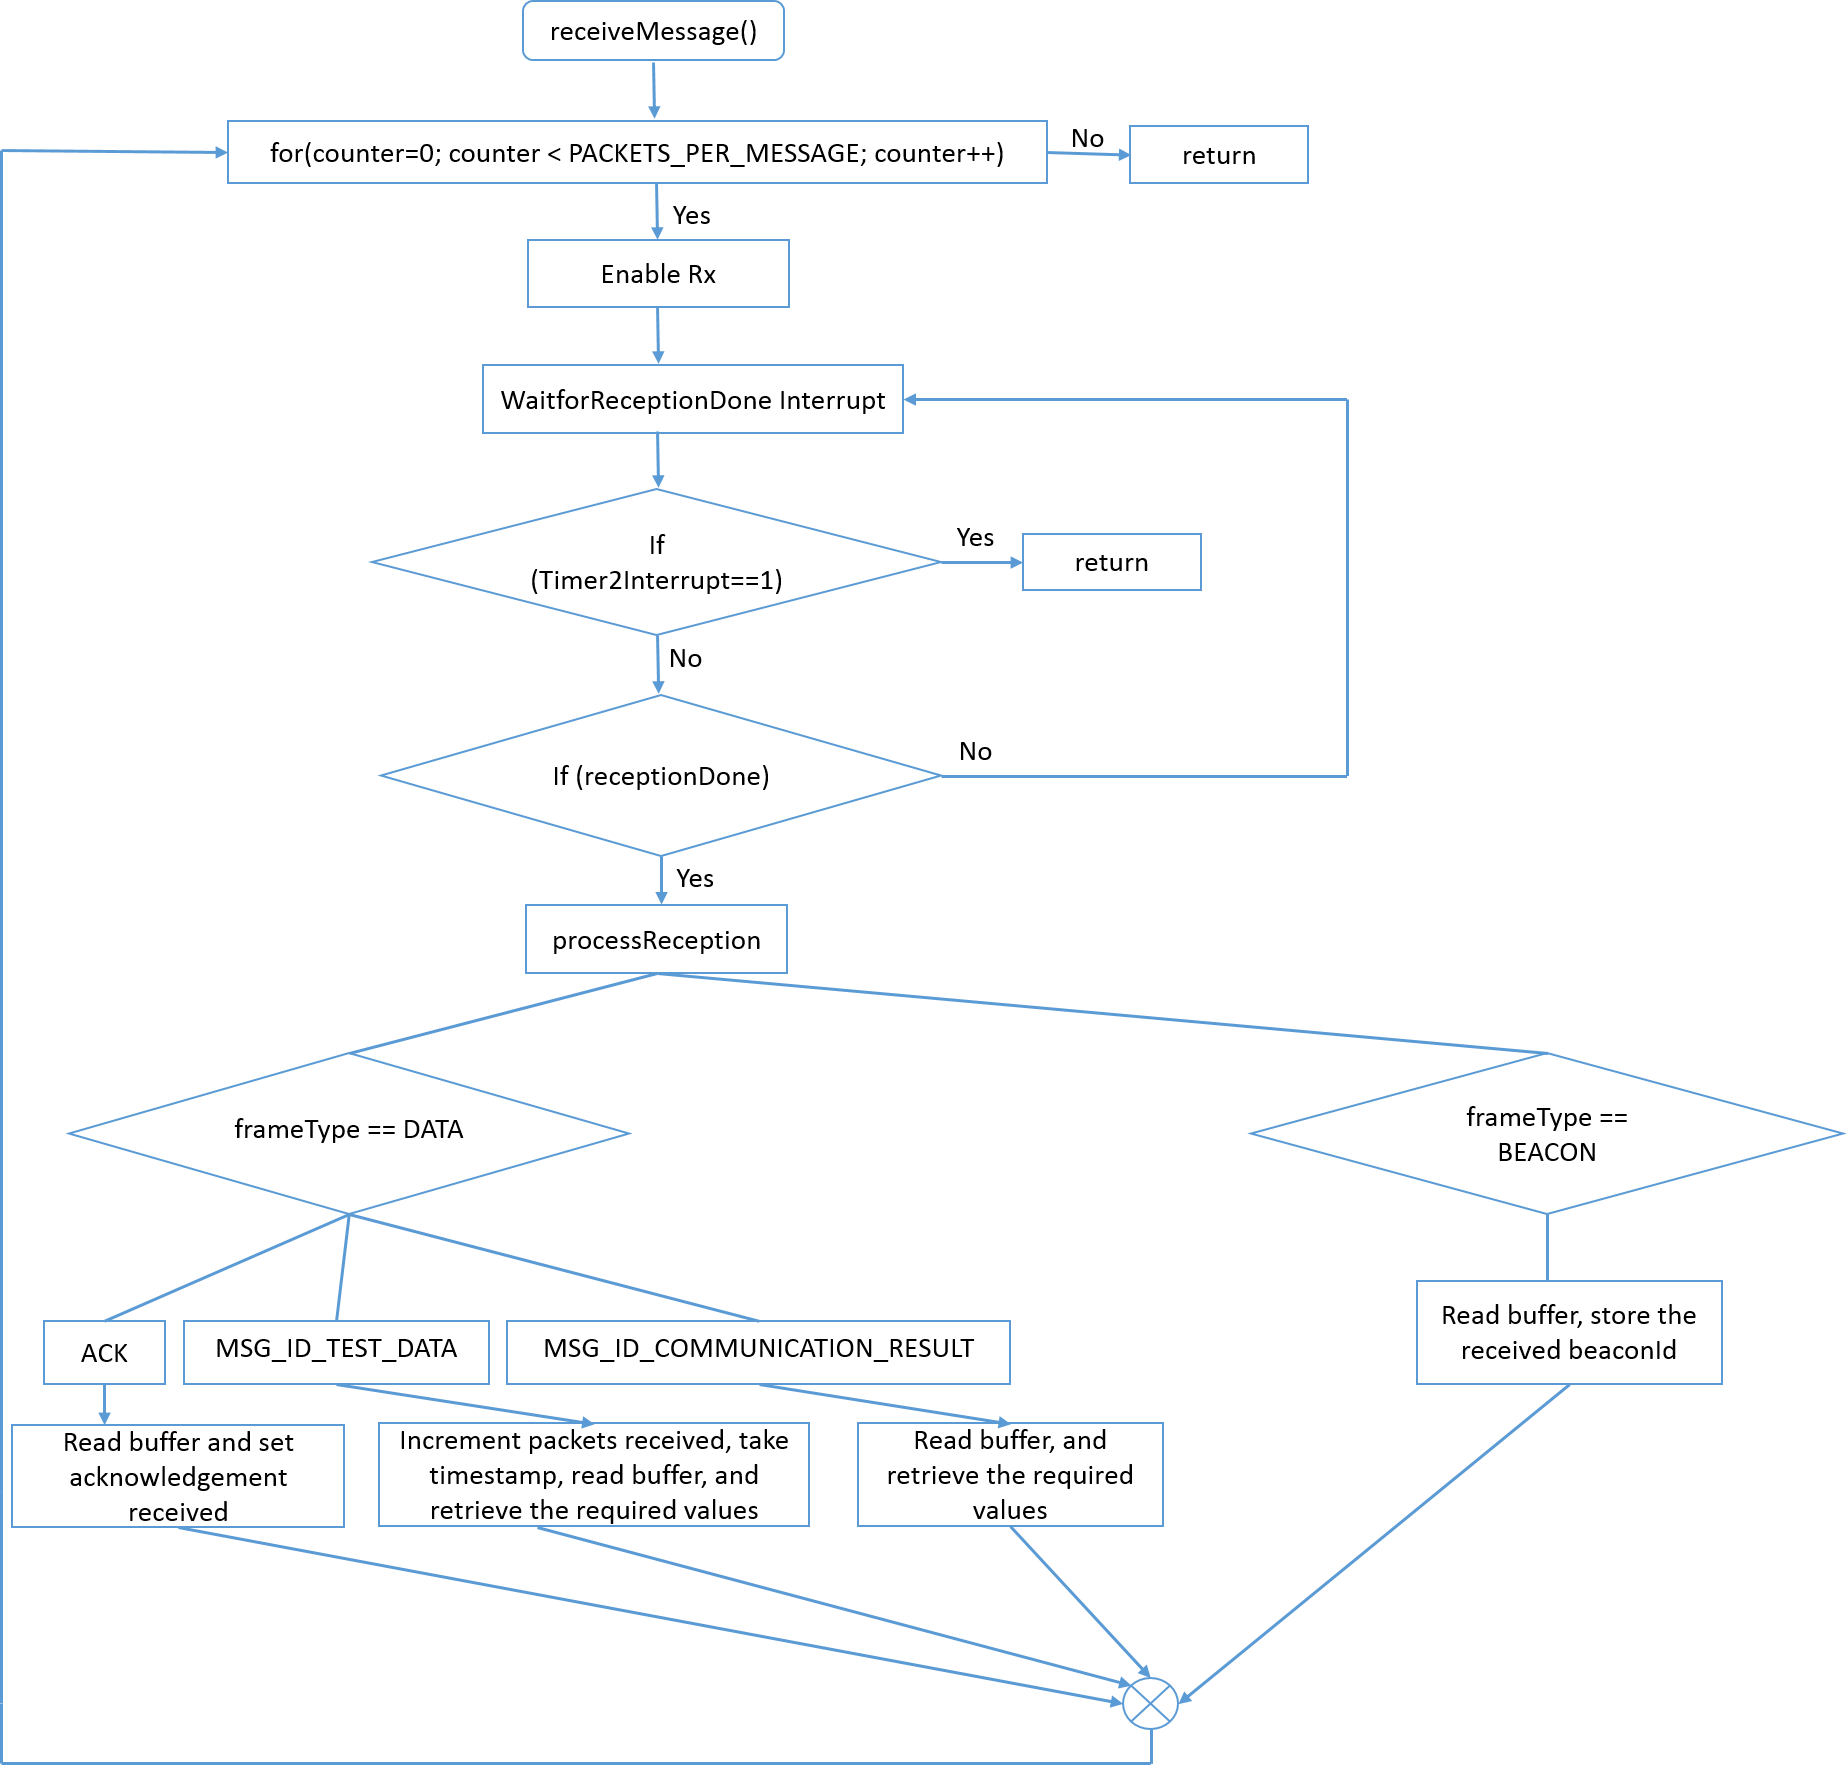
\includegraphics[width=1\textwidth]{figures/receiveMessage}
	\centering
	\caption{Process of reception of a message}
	\label{fig:receiveMessage}    
\end{figure}

\subsubsection{Transmission}
Now, let's consider in detail how the transmission works in the leading truck and the following truck which is indicated in the Figure \ref{fig:transmitMessage}. Inside a while loop, we check if the size of the payload is greater than 0. If so, we split the message into several 127-byte packets according to the IEEE 802.15.4 standard, copy the parts of a message appropriately to individual packets, take message timestamp and call \emph{writeToTxBuffer}. In \emph{writeToTxBuffer}, the transmission of MSG ID TEST DATA, MSG ID COMMUNICATION RESULT, and acknowledgment are handled in different ways. In the case of MSG ID TEST DATA we add the broadcast header, increase the sequence number, take the packet timestamp, transfer the packet and wait for the trasmitDone interrupt. In the case of MSG ID COMMUNICATION RESULT we add the broadcast header, increase the sequence number, transfer the packet and wait for the transmitDone Interrupt. Consequently, we enable RX and wait for three symbol durations for the reception of the acknowledgment. In the case of ACK, we add the broadcast header, transfer the acknowledgment packet and wait for the transmitDone interrupt. Once the size of the payload becomes 0, we exit from the while loop. In between two transmissions, we wait for 2 ms for successful reception of a packet at the receiver.


\subsubsection{Reception}
Figure \ref{fig:receiveMessage} shows how the reception is implemented. When the \emph{receiveMessage()} function is called, we enable the receiver for the first packet of a message and wait for the receptionDone interrupt. While waiting for the receptionDone interrupt, if the Timer2 interrupt occurs which indicates the reception timeout for that particular slot, we return and wait for the Timer1 interrupt, following which we transmit the next message according to the schedule. On the successful reception of the first packet of the message, we process the reception according to the type of the packet received. Since we can only differentiate between the BEACON and DATA message type, we identify the acknowledgment packet, test data and result communication packets based on the global volatile variables: acknow, final=false and final=true respectively. On reception of an acknowledgment packet, we read the buffer and set acknowledgment received to one. On the reception of a test data packet, we increment the number of packets received, take the time stamp, read the buffer and retrieve the required values. On the reception of communication result packet, we read the buffer and retrieve the required values. In the case of reception of a beacon packet, we read the buffer and store the received \emph{beaconId}. Once the reception of the first packet is processed, we enable reception for the second packet of a message, and the process repeats for all packets of a message and returns once all packets of a message are received or if the Timer2 interrupt occurs.

\subsubsection{Latency Calculation}    
We make use of Timer3 for the latency calculation. Figure \ref{fig:latencyCalculationLeadingTruck} and Figure \ref{fig:latencyCalculationFollowingTruck} show the latency calculation for the leading truck and following truck respectively. In order to obtain the message latency, we take the timestamp of the first packet of a message in the application layer before \emph{writeToTxBuffer} function is called and we take the timestamp of the last packet of a message in the application layer after obtaining its payloads, and take the difference between them.

For packet latency, we take the timestamp in the link layer for every packet, in the function \emph{writeToTxBuffer} before copying the payload to the broadcast payload, following which it is written to the transfer buffer and transmission started.  We take the timestamp in the link layer once the same packet has reached the other node, in the function \emph{processReception} that is called after a reception interrupt is handled. 

In Figure \ref{fig:latencyCalculationLeadingTruck}, the x-axis denotes the time, the top part of the figure indicates the leading truck and the bottom part of the figure indicates the following truck. The figure depicts the scenario of two packets per message being sent from the leading truck to the following truck. The message latency is the difference of timestamp $t6$ in the following truck and timestamp $t1$ in the leading truck. The packet latency is the difference of timestamp $t4$ in the following truck and timestamp $t2$ in the leading truck or difference of timestamp $t5$ in the following truck and timestamp $t3$ in the leading truck.

Similarly, the calculation of message latency and packet latency for the following truck is shown in the Figure \ref{fig:latencyCalculationFollowingTruck} wherein a message is transmitted from the following truck to the leading truck.
\begin{figure}[h!]
    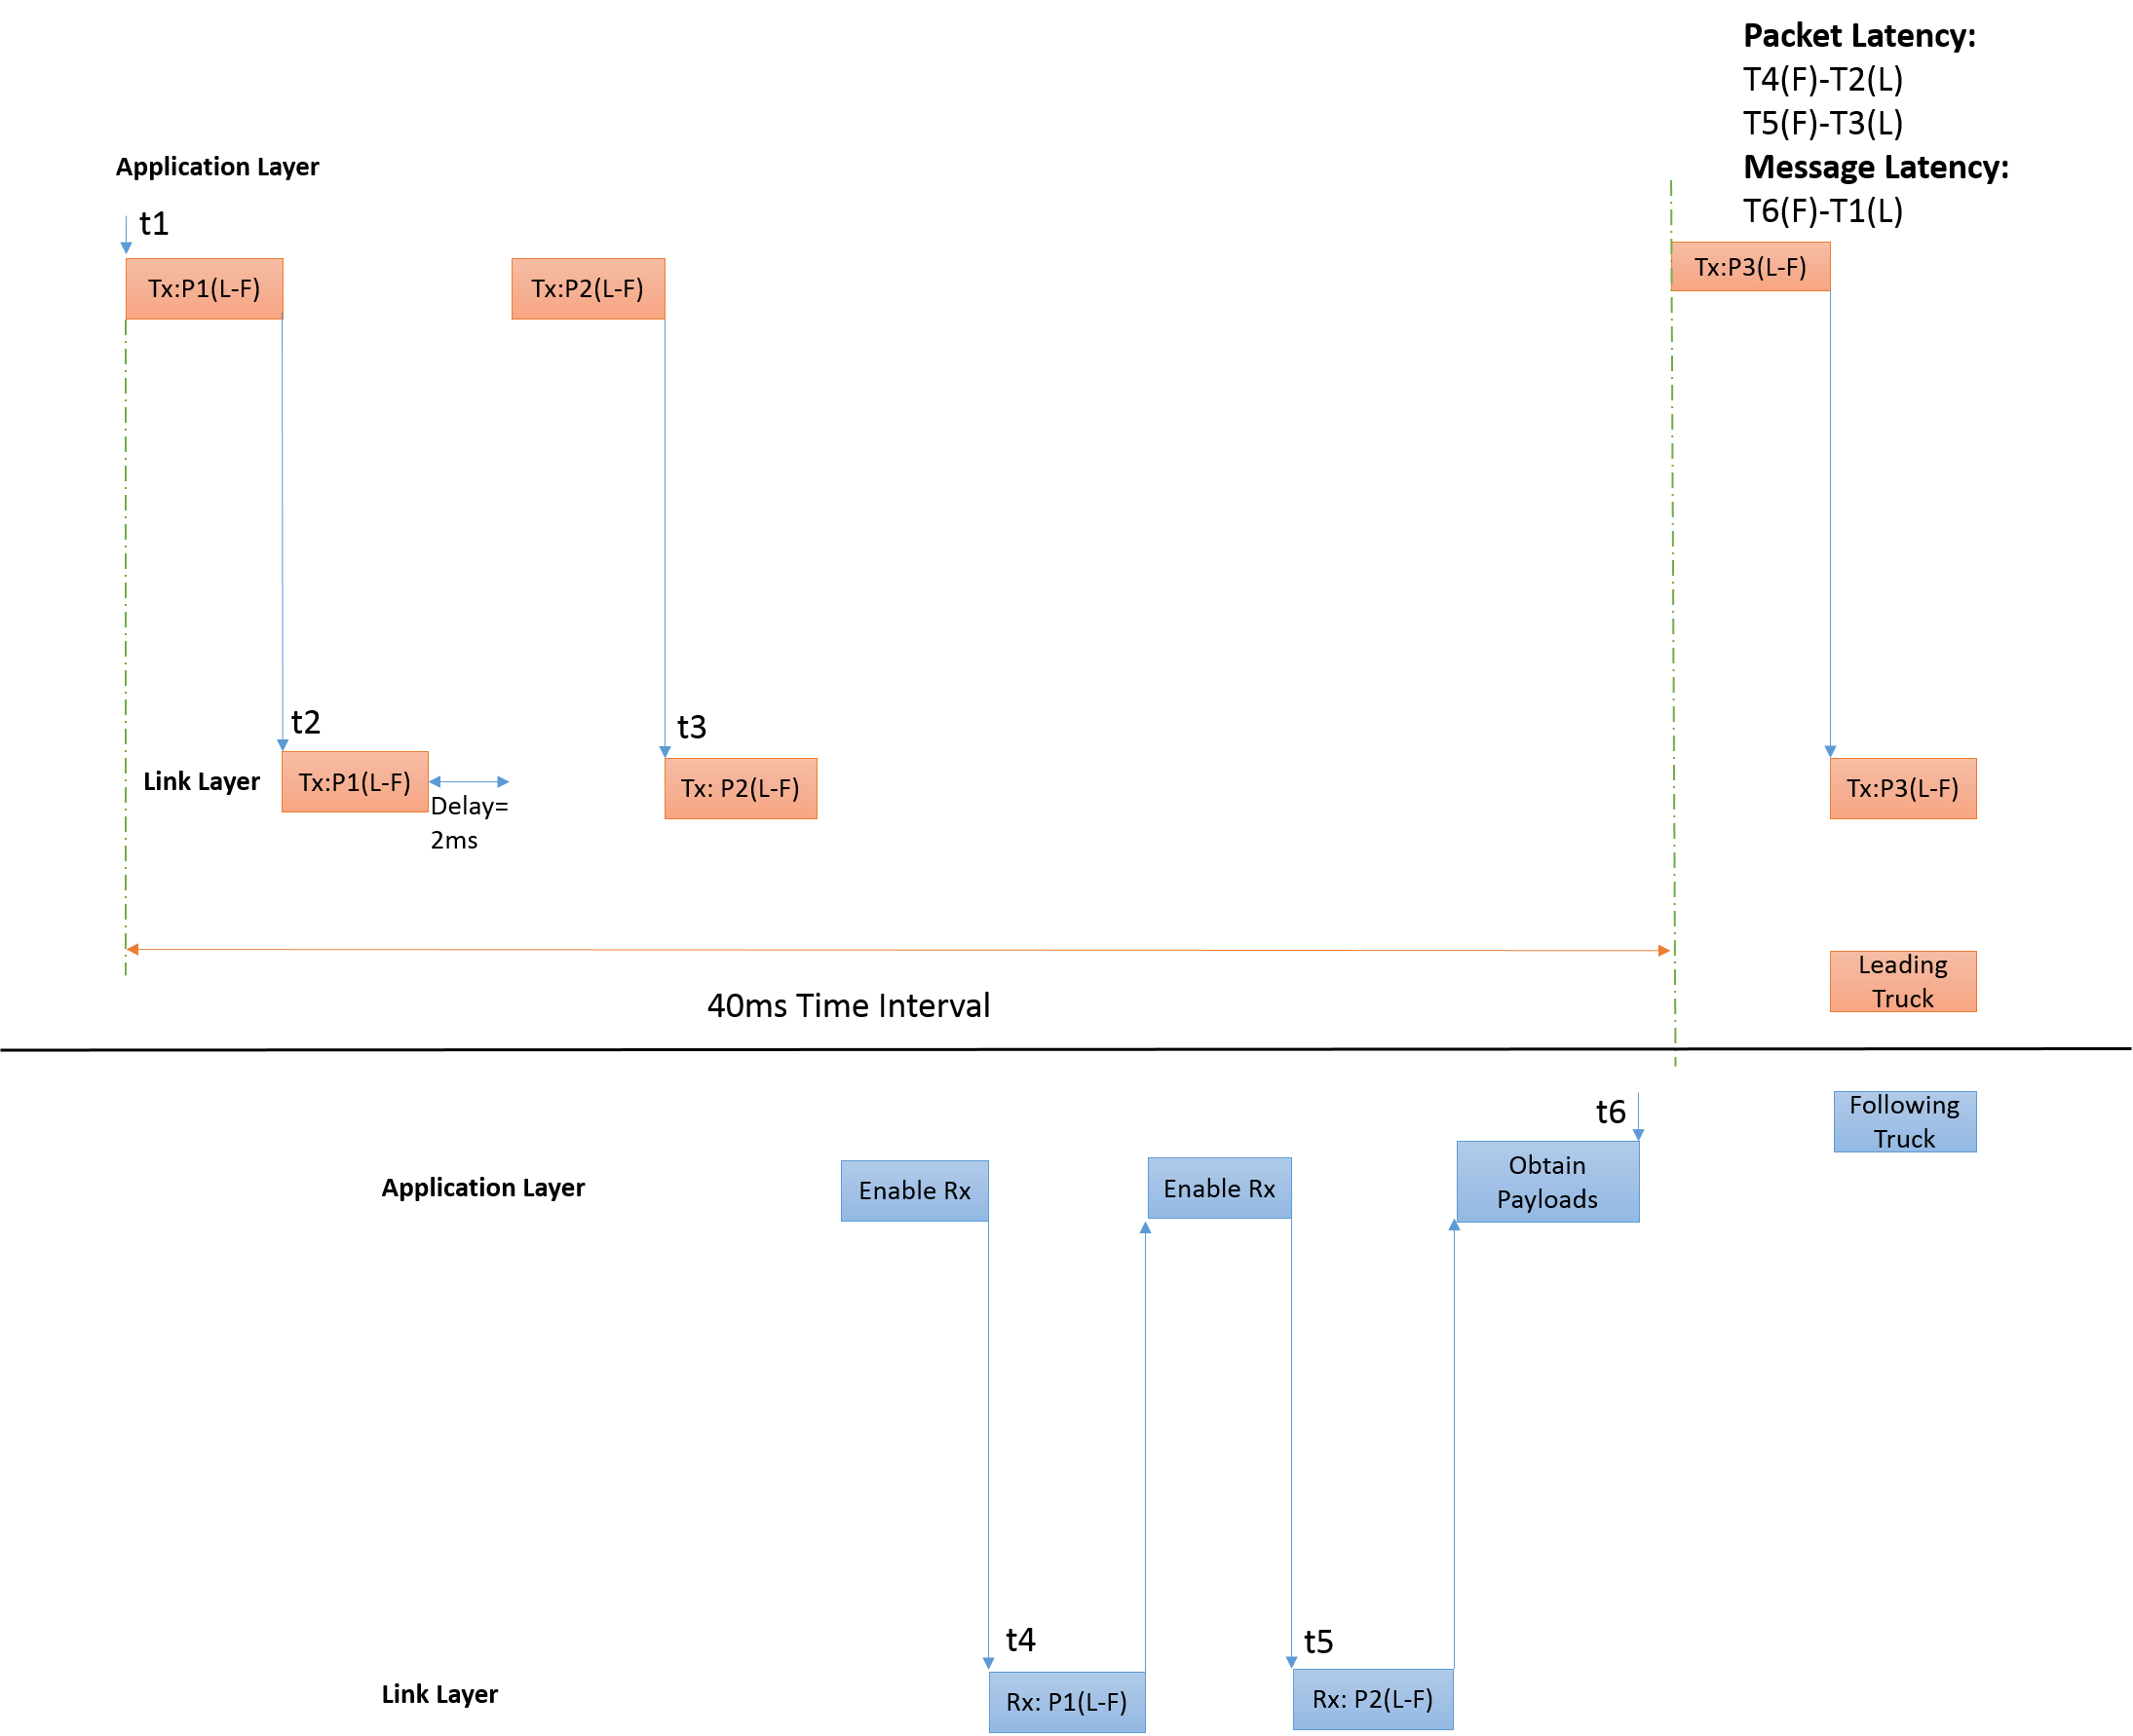
\includegraphics[width=1\textwidth]{figures/LatencyCalculationLeadingTruck}
    \centering
    \caption{Latency Calculation - Leading Truck}
    \label{fig:latencyCalculationLeadingTruck}    
\end{figure}

\begin{figure}[h!]
	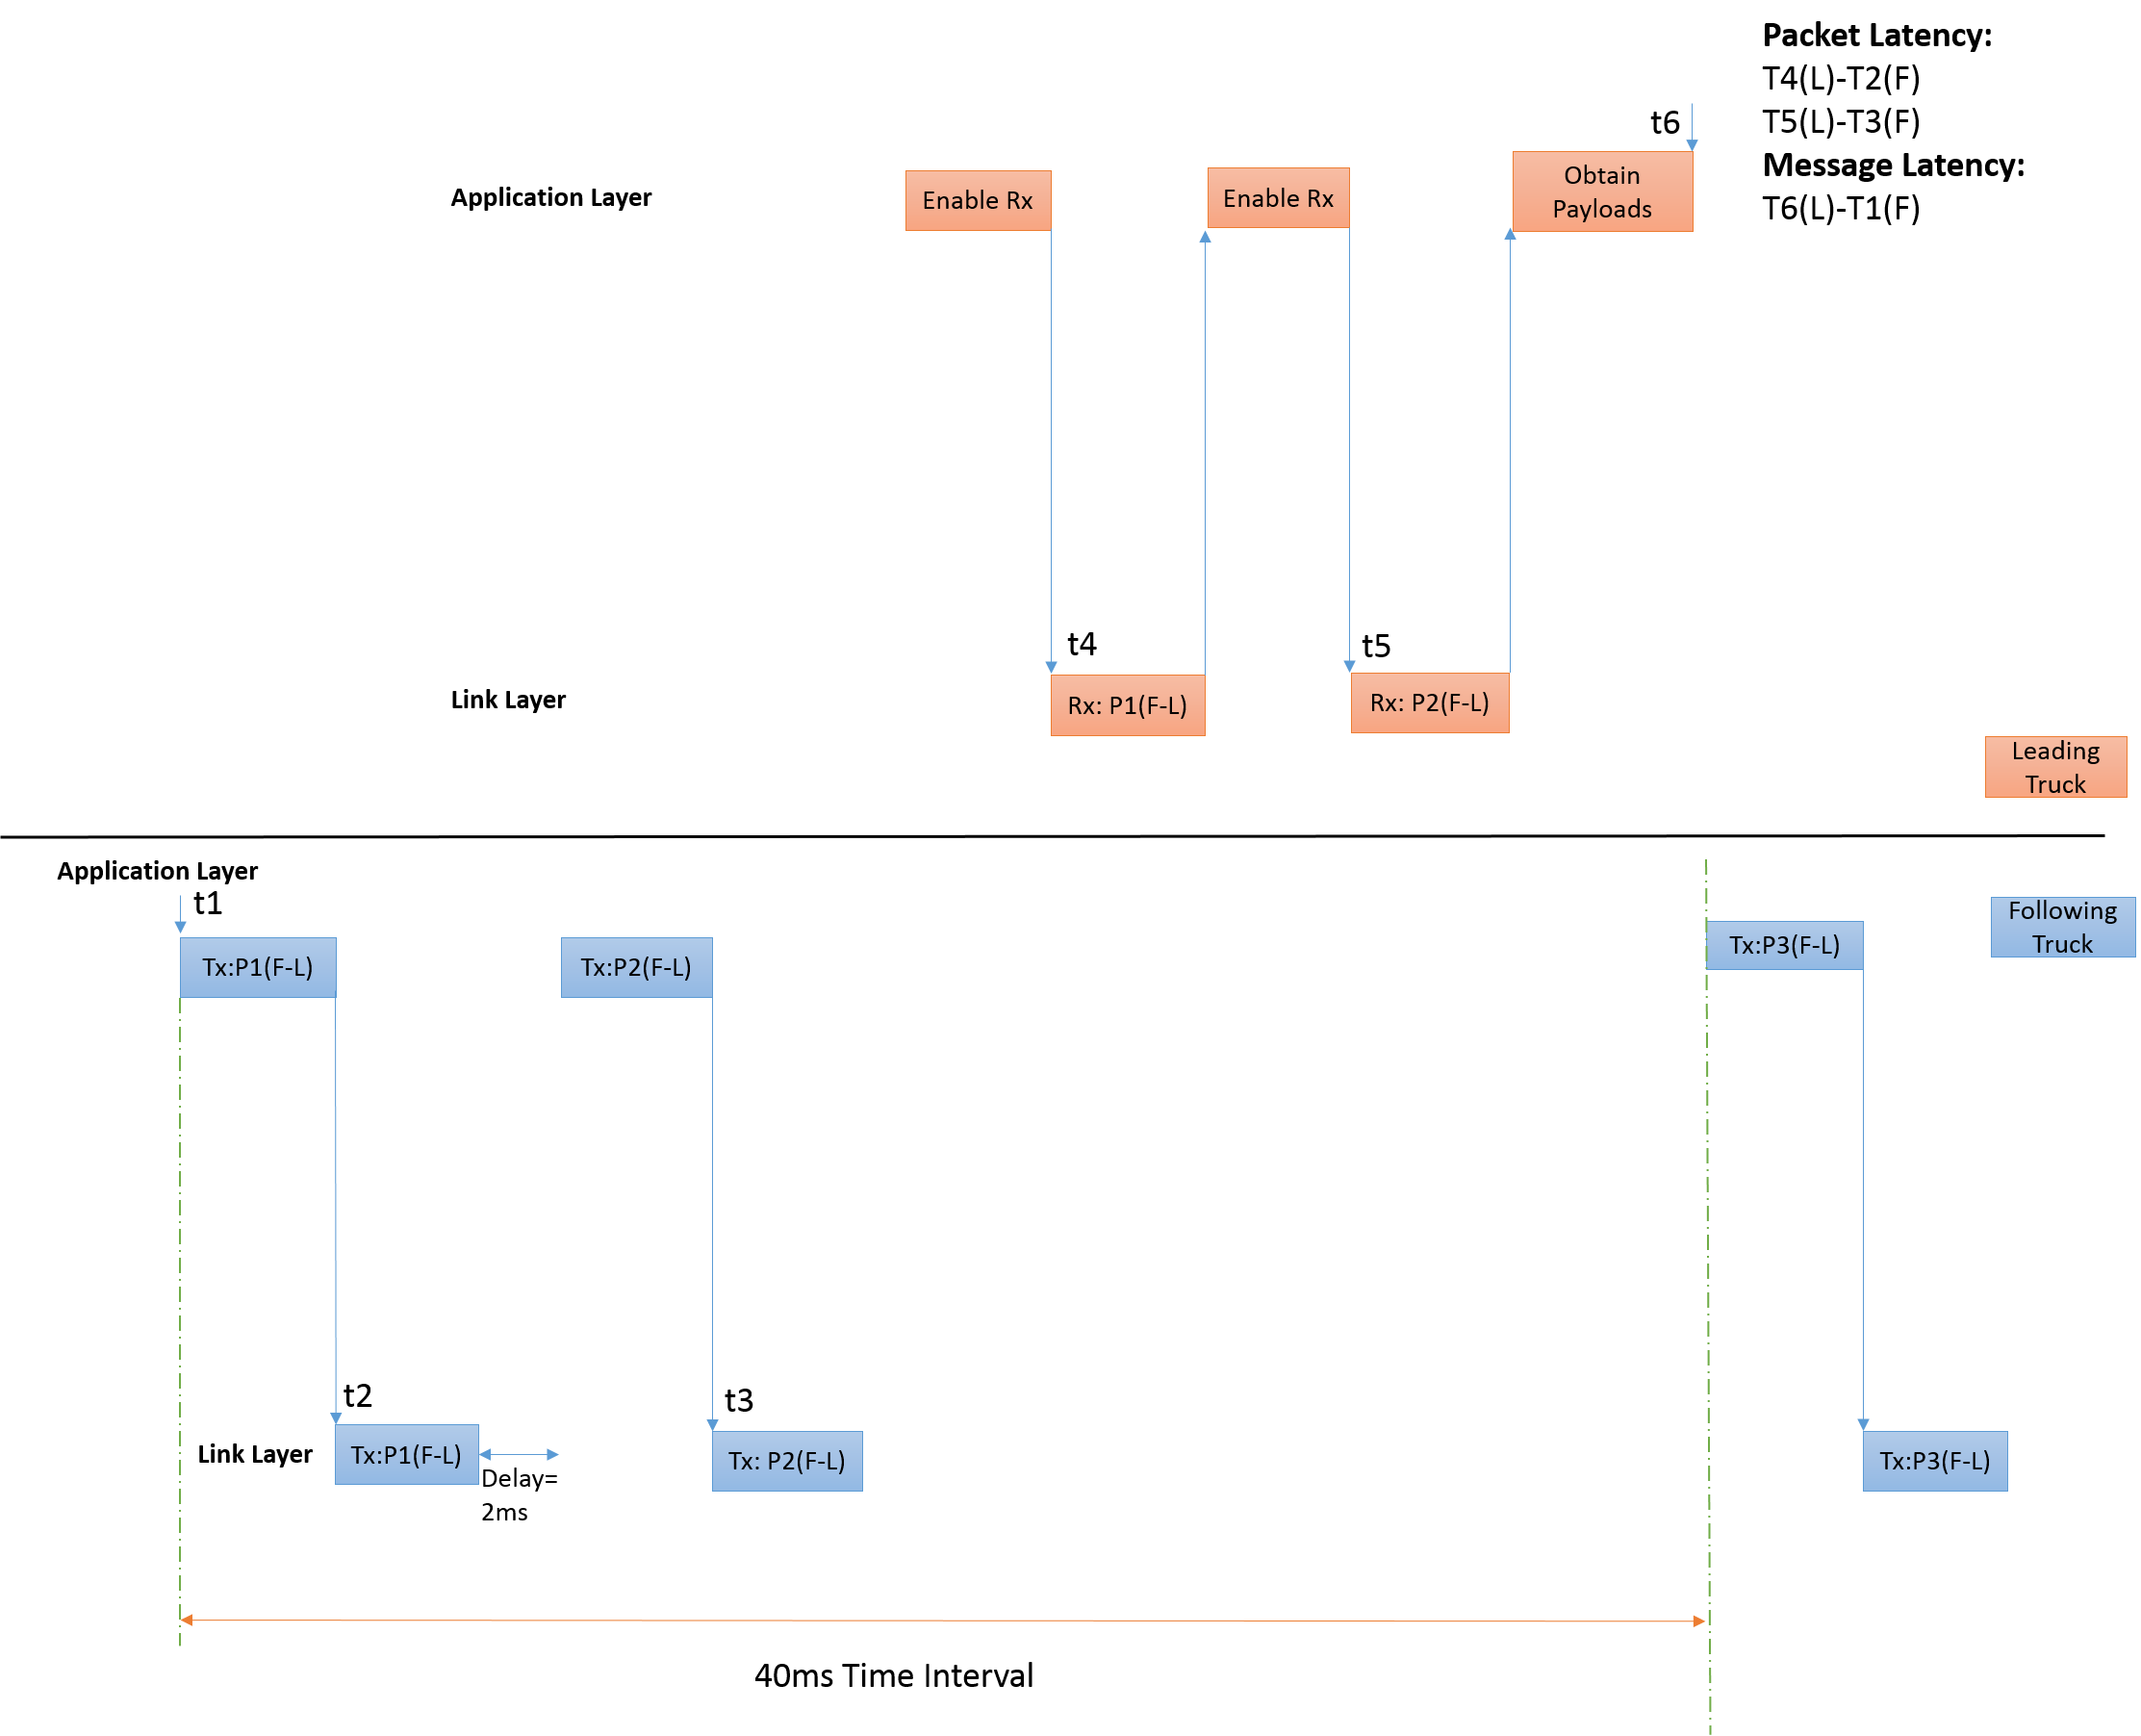
\includegraphics[width=1\textwidth]{figures/LatencyCalculationFollowingTruck}
	\centering
	\caption{Latency Calculation - Following Truck}
	\label{fig:latencyCalculationFollowingTruck}    
\end{figure}

\begin{figure}[h!]
	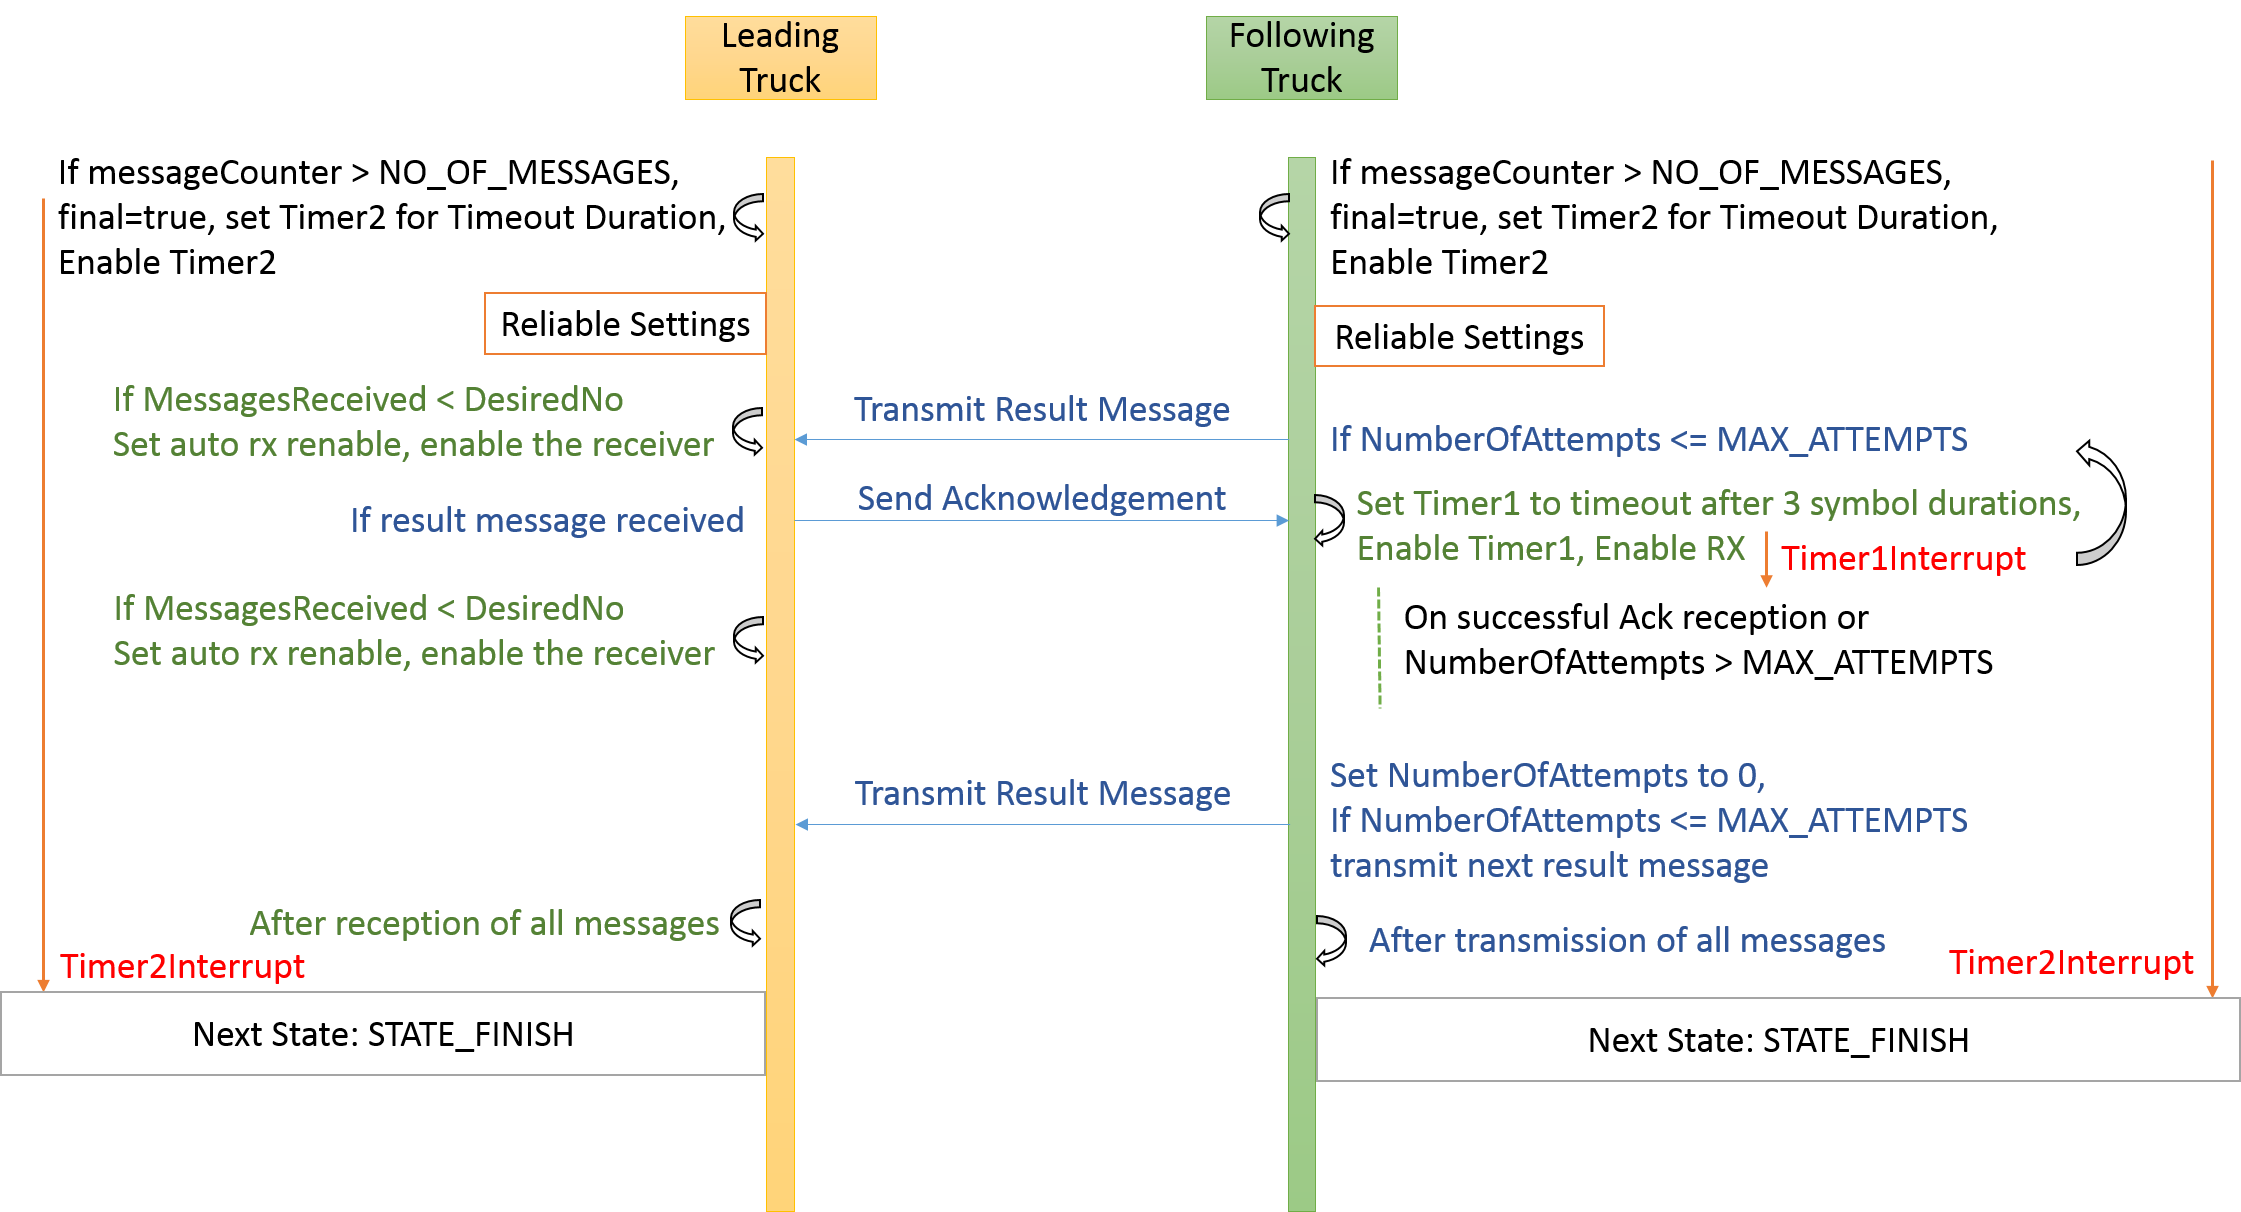
\includegraphics[width=1\textwidth]{figures/StateResultDetermination}
	\centering
	\caption{State Result Determination}
	\label{fig:StateResultDetermination}    
\end{figure}

\subsection{State Result Communication}
The working of State Result Communication is indicated in the Figure \ref{fig:StateResultDetermination}. If messageCounter \textgreater \emph{NO\_OF\_MESSAGES}, we set final=true and enter State Result Communication in both nodes. It is to be noted that the leading truck enters this state earlier than the following truck because of the 20 ms offset in the following truck. We set Timer2 for the timeout duration for the entire phase and enable timer2. We make use of the reliable settings in this phase, wherein we use the lowest data rate of 110 kbps and make use of acknowledgment for each log sent in this phase. 

In the case of the following truck, for a particular log, we define \emph{MAX\_ATTEMPTS} as the number of times to repeat sending that particular log until an acknowledgment is received. If the number of attempts is less than or equal to the \emph{MAX\_ATTEMPTS}, we transmit that particular log. Following which, we set Timer1 to timeout after three symbol durations, enable Timer1 and enable receiver for the reception of acknowledgment. On the occurrence of Timer1 interrupt, we increment the number of attempts, go back and transmit that particular log again if the number of attempts is less than or equal to the \emph{MAX\_ATTEMPTS}. On the reception of acknowledgment, we set the number of attempts to 0 and transmit the next result log if the number of attempts is less than or equal to \emph{MAX\_ATTEMPTS}. This process continues for all the result logs, and it enters the next phase STATE FINISH after transmission of all logs or if Timer2 interrupt occurs.

In the case of the leading truck, if the number of logs received is less than \emph{DesiredNo} we set \emph{autorxreenable} and enable the receiver. If the result log is received, we process that particular log and send an acknowledgment back. Following which we set \emph{autorxreenable} and enable the receiver if the number of messages received is less than \emph{DesiredNo}. This process continues for the reception of all the logs and it enters the next phase STATE FINISH after the reception of all logs or if Timer2 interrupt occurs. The test log structure definition is shown in Listing \ref{lst:testLogStructureDefinition}. Using the stored values of this structure for each log, a comma separated string is created as shown in Listing \ref{lst:loggingFormat} and printed on the laptop/computer using serial communication, which is further processed in MATLAB.

\begin{lstlisting}[caption={Logging Format},
label={lst:loggingFormat}, language=C]
Log,tseqno1,0,tseqno2,1,tseqno3,2,tseqno4,3,rseqno1,0,rseqno2,1,rseqno3,2,rseqno4,3,messageLatency,8.950,packetLatency1,0.843,packetLatency2,0.843,packetLatency3,0.843,packetLatency4,0.829,distance,0.00,C1,955,C2,1015,C3,1028,C4,925,N1,236,N2,236,N3,235,N4,229,F11,2716,F12,2385,F13,2883,F14,2420,F21,3033,F22,3369,F23,3040,F24,3099,F31,2971,F32,2439,F33,2869,F34,2290
\end{lstlisting}

\vspace{2cm}
\begin{lstlisting}[caption={Test Log structure definition}, label={lst:testLogStructureDefinition}, language=C]
typedef struct {
uint16_t tseqNo[PACKETS_PER_MESSAGE];
uint16_t rseqNo[PACKETS_PER_MESSAGE];
uint32_t messageLatency;
uint32_t packetLatency[PACKETS_PER_MESSAGE];
double distance;
uint16_t stdNoise[PACKETS_PER_MESSAGE];
uint16_t C[PACKETS_PER_MESSAGE];
uint16_t N[PACKETS_PER_MESSAGE];
uint16_t F1[PACKETS_PER_MESSAGE];
uint16_t F2[PACKETS_PER_MESSAGE];
uint16_t F3[PACKETS_PER_MESSAGE];
}logging;
\end{lstlisting}





\subsection{State Finish}
In the phase STATE FINISH, we reset for the next configuration and stop the link. Wherein we disable all interrupts which were set in STATE START, disable all the three timers, reset them and reset the transceiver. If the number of times to repeat is less than (NO OF TIMES TO RUN * NUM OF DW1000 CONFIGS) we load the next configuration ((configuration + 1) \% NUM OF DW1000 CONFIGS) and return to STATE START, else we stop the execution.

\subsection{Ranging Method}
For the implementation of ranging, we make use of Double-Sided Two-Way Ranging (DS-TWR), which is an extension of the basic single-sided two-way ranging in which two round trip time measurements are used and combined to give a time-of-flight result which has a reduced error even for quite long response delays. The operation of DS-TWR used in our implementation is shown in Figure \ref{fig:rangingMethod}. The leading truck sends a POLL packet to the following truck, for which the following truck sends a response packet to the leading truck. Consequently, the leading truck sends a final packet to the following truck. Lastly, the following truck sends the result packet to the leading truck with all the required time stamps from the following truck (POLL RX time stamp, RESPONSE TX time stamp and FINAL RX time stamp). The leading truck makes use of the time stamps sent in the result packet and its own time stamps (POLL TX time stamp, RESPONSE RX time stamp and FINAL TX time stamp) to calculate the time-of-flight estimate according to  Equation \ref{eq:tofestimate}. Using this time-of-flight estimate, distance is calculated according to  Equation \ref{eq:distanceEstimate}.

\begin{equation}
\label{eq:tofestimate}
T_{prop}=\dfrac{T_{round1}*T_{round2}-T_{reply1}*T_{reply2}}{T_{round1}+T_{round2}+T_{reply1}+T_{reply2}}
\end{equation}

\begin{equation}
\label{eq:distanceEstimate}
Distance = T_{prop} * SPEED\_OF\_LIGHT
\end{equation}

\begin{figure}[h!]
    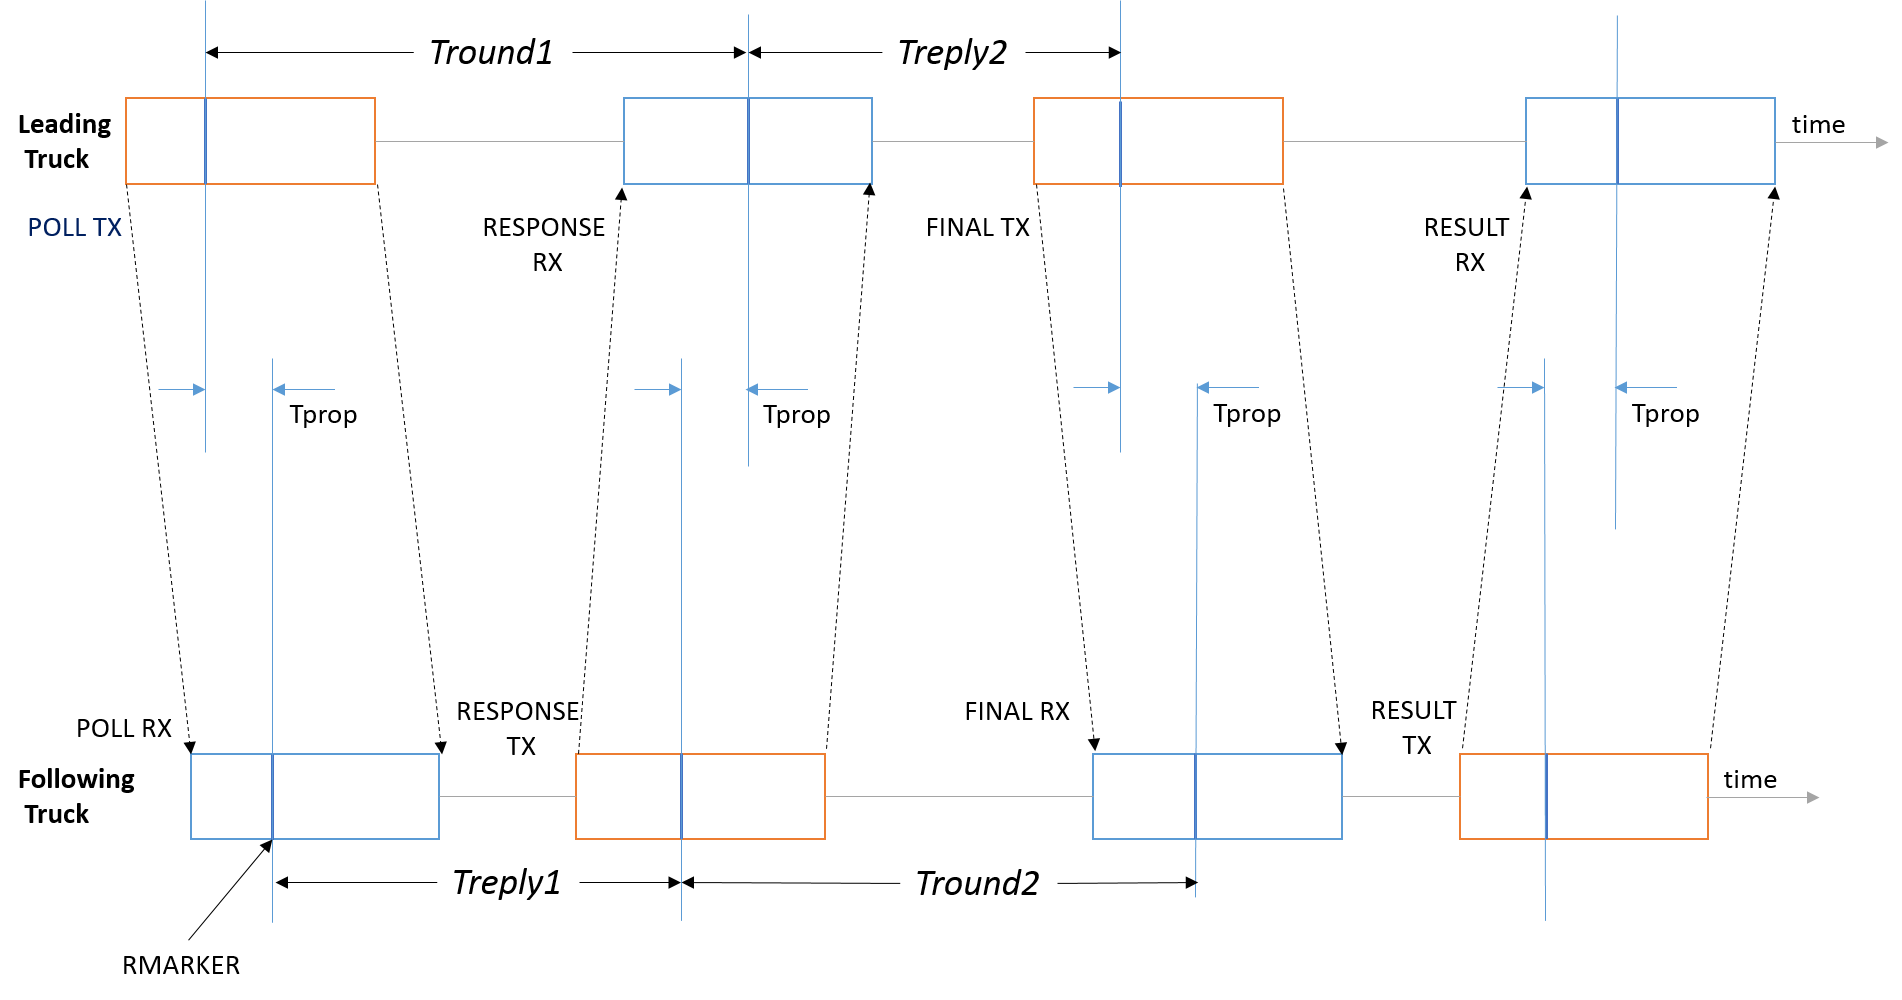
\includegraphics[width=1\textwidth]{figures/RangingMethod}
    \centering
    \caption{Ranging Method}
    \label{fig:rangingMethod}    
\end{figure}

\subsection{Ranging Implementation}
Figure \ref{fig:implementationOfRanging} shows how we integrate ranging along with communication. We refer to the last packet of a message to send/receive ranging related information. Initially, we reset the parameters for range calculation in both the leading truck and the following truck. 

In the case of the following truck, on the reception of ranging POLL information, it resets the parameters and gets the POLL RX time stamp. It sends the ranging RESPONSE information when \emph{rangeType}\%2==0. On the reception of the ranging FINAL information, it gets the RESPONSE TX time stamp and the FINAL RX time stamp. It sends the ranging RESULT information along with the POLL RX time stamp, the RESPONSE TX time stamp and the FINAL RX time stamp when \emph{rangeType}\%2==1.

In the case of the leading truck, it sends the Ranging POLL information when \emph{rangeType}\%2==0. On reception of the ranging RESPONSE information from the following truck, it resets the parameters and gets the POLL TX time stamp and the RESPONSE RX time stamp. It sends the ranging FINAL information when \emph{rangeType}\%2==1. On reception of the ranging RESULT information from the following truck, it gets the FINAL TX time stamp, retrieves the POLL RX time stamp, the RESPONSE TX time stamp and the FINAL RX time stamp from the ranging RESULT information and calculates the distance between the trucks. The reset of the parameters is done to ensure the distance is calculated appropriately even in the case of packet loss. To calculate the distance, the time-of-flight estimate calculated according to the equation \ref{eq:tofestimate} is multiplied by DWT TIME UNITS since these time stamps are given by the DecaWave device and finally the distance is calculated according to the equation \ref{eq:distanceEstimate}.
   
\begin{figure}[h!]
    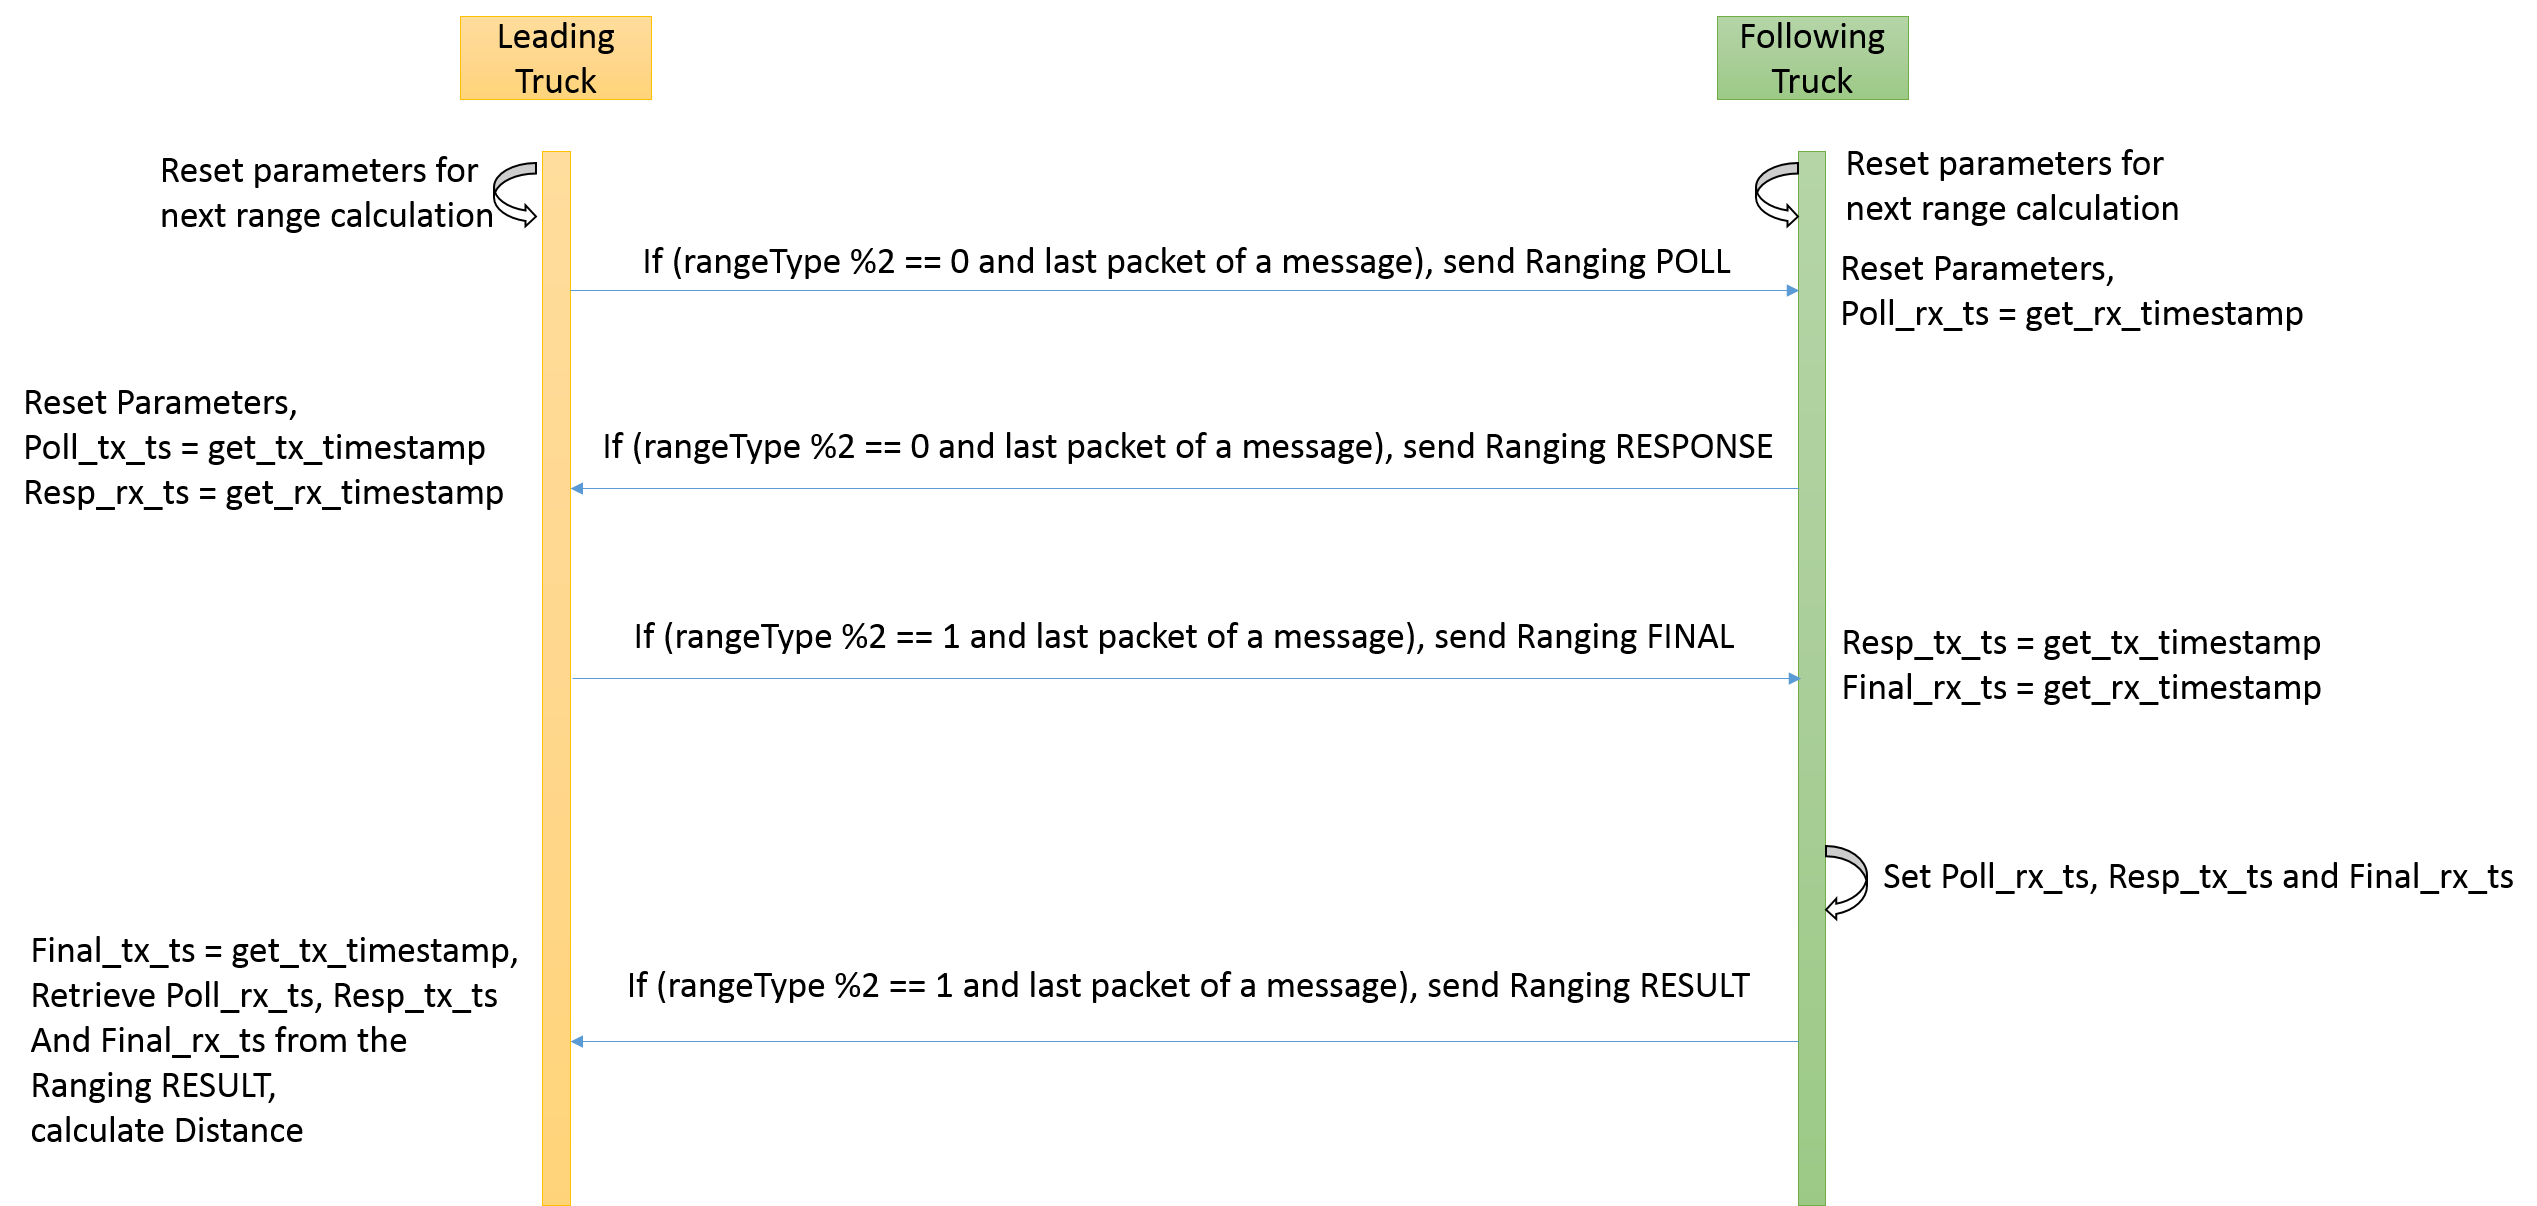
\includegraphics[width=1\textwidth]{figures/RangingCalculation}
    \centering
    \caption{Implementation of Ranging}
    \label{fig:implementationOfRanging}    
\end{figure}

\vspace{2cm}

\subsection{Cross Verification of Design}

To cross verify if the system is designed accurately, additional parameters were logged for the packets as shown in Listing \ref{lst:testLogStructureVerificationOfDesign} in the unit testing phase. An indication of the parameters logged is provided in Figure \ref{fig:LoggedParametersDetermineAppWorking}. 
\begin{lstlisting}[caption={Test Log structure for verification of design}, label={lst:testLogStructureVerificationOfDesign}, language=C]
typedef struct {
uint16_t tseqNo[PACKETS_PER_MESSAGE];
uint16_t rseqNo[PACKETS_PER_MESSAGE];
uint32_t tonTimePacket[4];
uint32_t ronTimePacket[4];
uint32_t tcompletiontimePacket[4];
uint32_t rcompletiontimePacket[4];
uint32_t messageLatency;
uint32_t packetLatency[PACKETS_PER_MESSAGE];
uint8_t timeout[PACKETS_PER_MESSAGE];
uint32_t errorcompletiontimePacket[4];
double distance;
uint16_t stdNoise[PACKETS_PER_MESSAGE];
uint16_t C[PACKETS_PER_MESSAGE];
uint16_t N[PACKETS_PER_MESSAGE];
uint16_t F1[PACKETS_PER_MESSAGE];
uint16_t F2[PACKETS_PER_MESSAGE];
uint16_t F3[PACKETS_PER_MESSAGE];
} logging;
\end{lstlisting}
Here the parameter 'timeout' indicates if a timeout occurred during the reception of a packet and 'errorcompletiontimePacket' indicates the timestamp if any errors like Rx Frame timeout, Rx SFD timeout, Rx Preamble timeout, RX PHR error, Rx Reed-Solomon error (Sync loss),or Rx Bad CRC occur. Using these parameters we checked if the receiver of the following truck is turned on before the transmission from the leading truck for every packet of a message and similarly we checked if the receiver of the leading truck is turned on before the transmission from the following truck for every packet of a message. We also checked if the time between the transmission of packets was 2 ms and the time between the reception completion of one packet and enablement of reception for the next packet is less than 2 ms. We verified if the system worked as designed during timeouts or when errors occurred. We also verified that the nodes are synchronized when they enter the communication phase through an oscilloscope by creating a pulse on the GPIO Pin on entering the communication phase. It was observed that the difference in synchronization was less than 200 $\mu$s, which is ok for our application.

During the cross verification of the design, two major issues were found when the code was run for long durations of time. The first issue was that the schedule of transmission was getting affected in few cases wherein the receiver of the following truck was not getting turned on before the transmission of a packet from the leading truck and vice versa. This error was not reproducible and hence it was tough to identify the source of the problem. To solve this problem, flags were used to identify in what phase the node was when Timer1 interrupt of 40 ms occurred. It was observed that the node was always in the logging state when Timer1 occurred. At that point of time when this error occurred, the sequence of the code was to transmit a message, receive a message, log that particular message and then go to the next transmission. Having identified that the issue was associated with logging, we turned off all logging and printed an error only if a packet reception was missed. We found that the code worked as desired. Digging deep into the issue we found that the issue was associated with the COM port interrupts interfering with the Timer1 and Timer2 Interrupts. To solve this issue, we stored all the logging information in a structure array and handled the printing of the log after the communication phase.

Another issue that was identified is that the code crashed at times. This error too was not reproducible. The approach used to solve this issue was to store values of certain variables in RAM and print the values of these variables on pressing reset after the crash occurred. To do this, we changed the settings in LPCXpresso IDE to trick the microcontroller to believe that there is lesser memory space available while creating the makefile and used that part of memory for storing the values of these variables. It was identified that the issue was caused due to the reception of an unexpected packet which could occur if the reception and timeout interrupt occurred at the same point in time. This exception was handled to solve this problem, and the system was cross-verified for the designed functioning before going into the experimentation.

\begin{figure}[h!]
    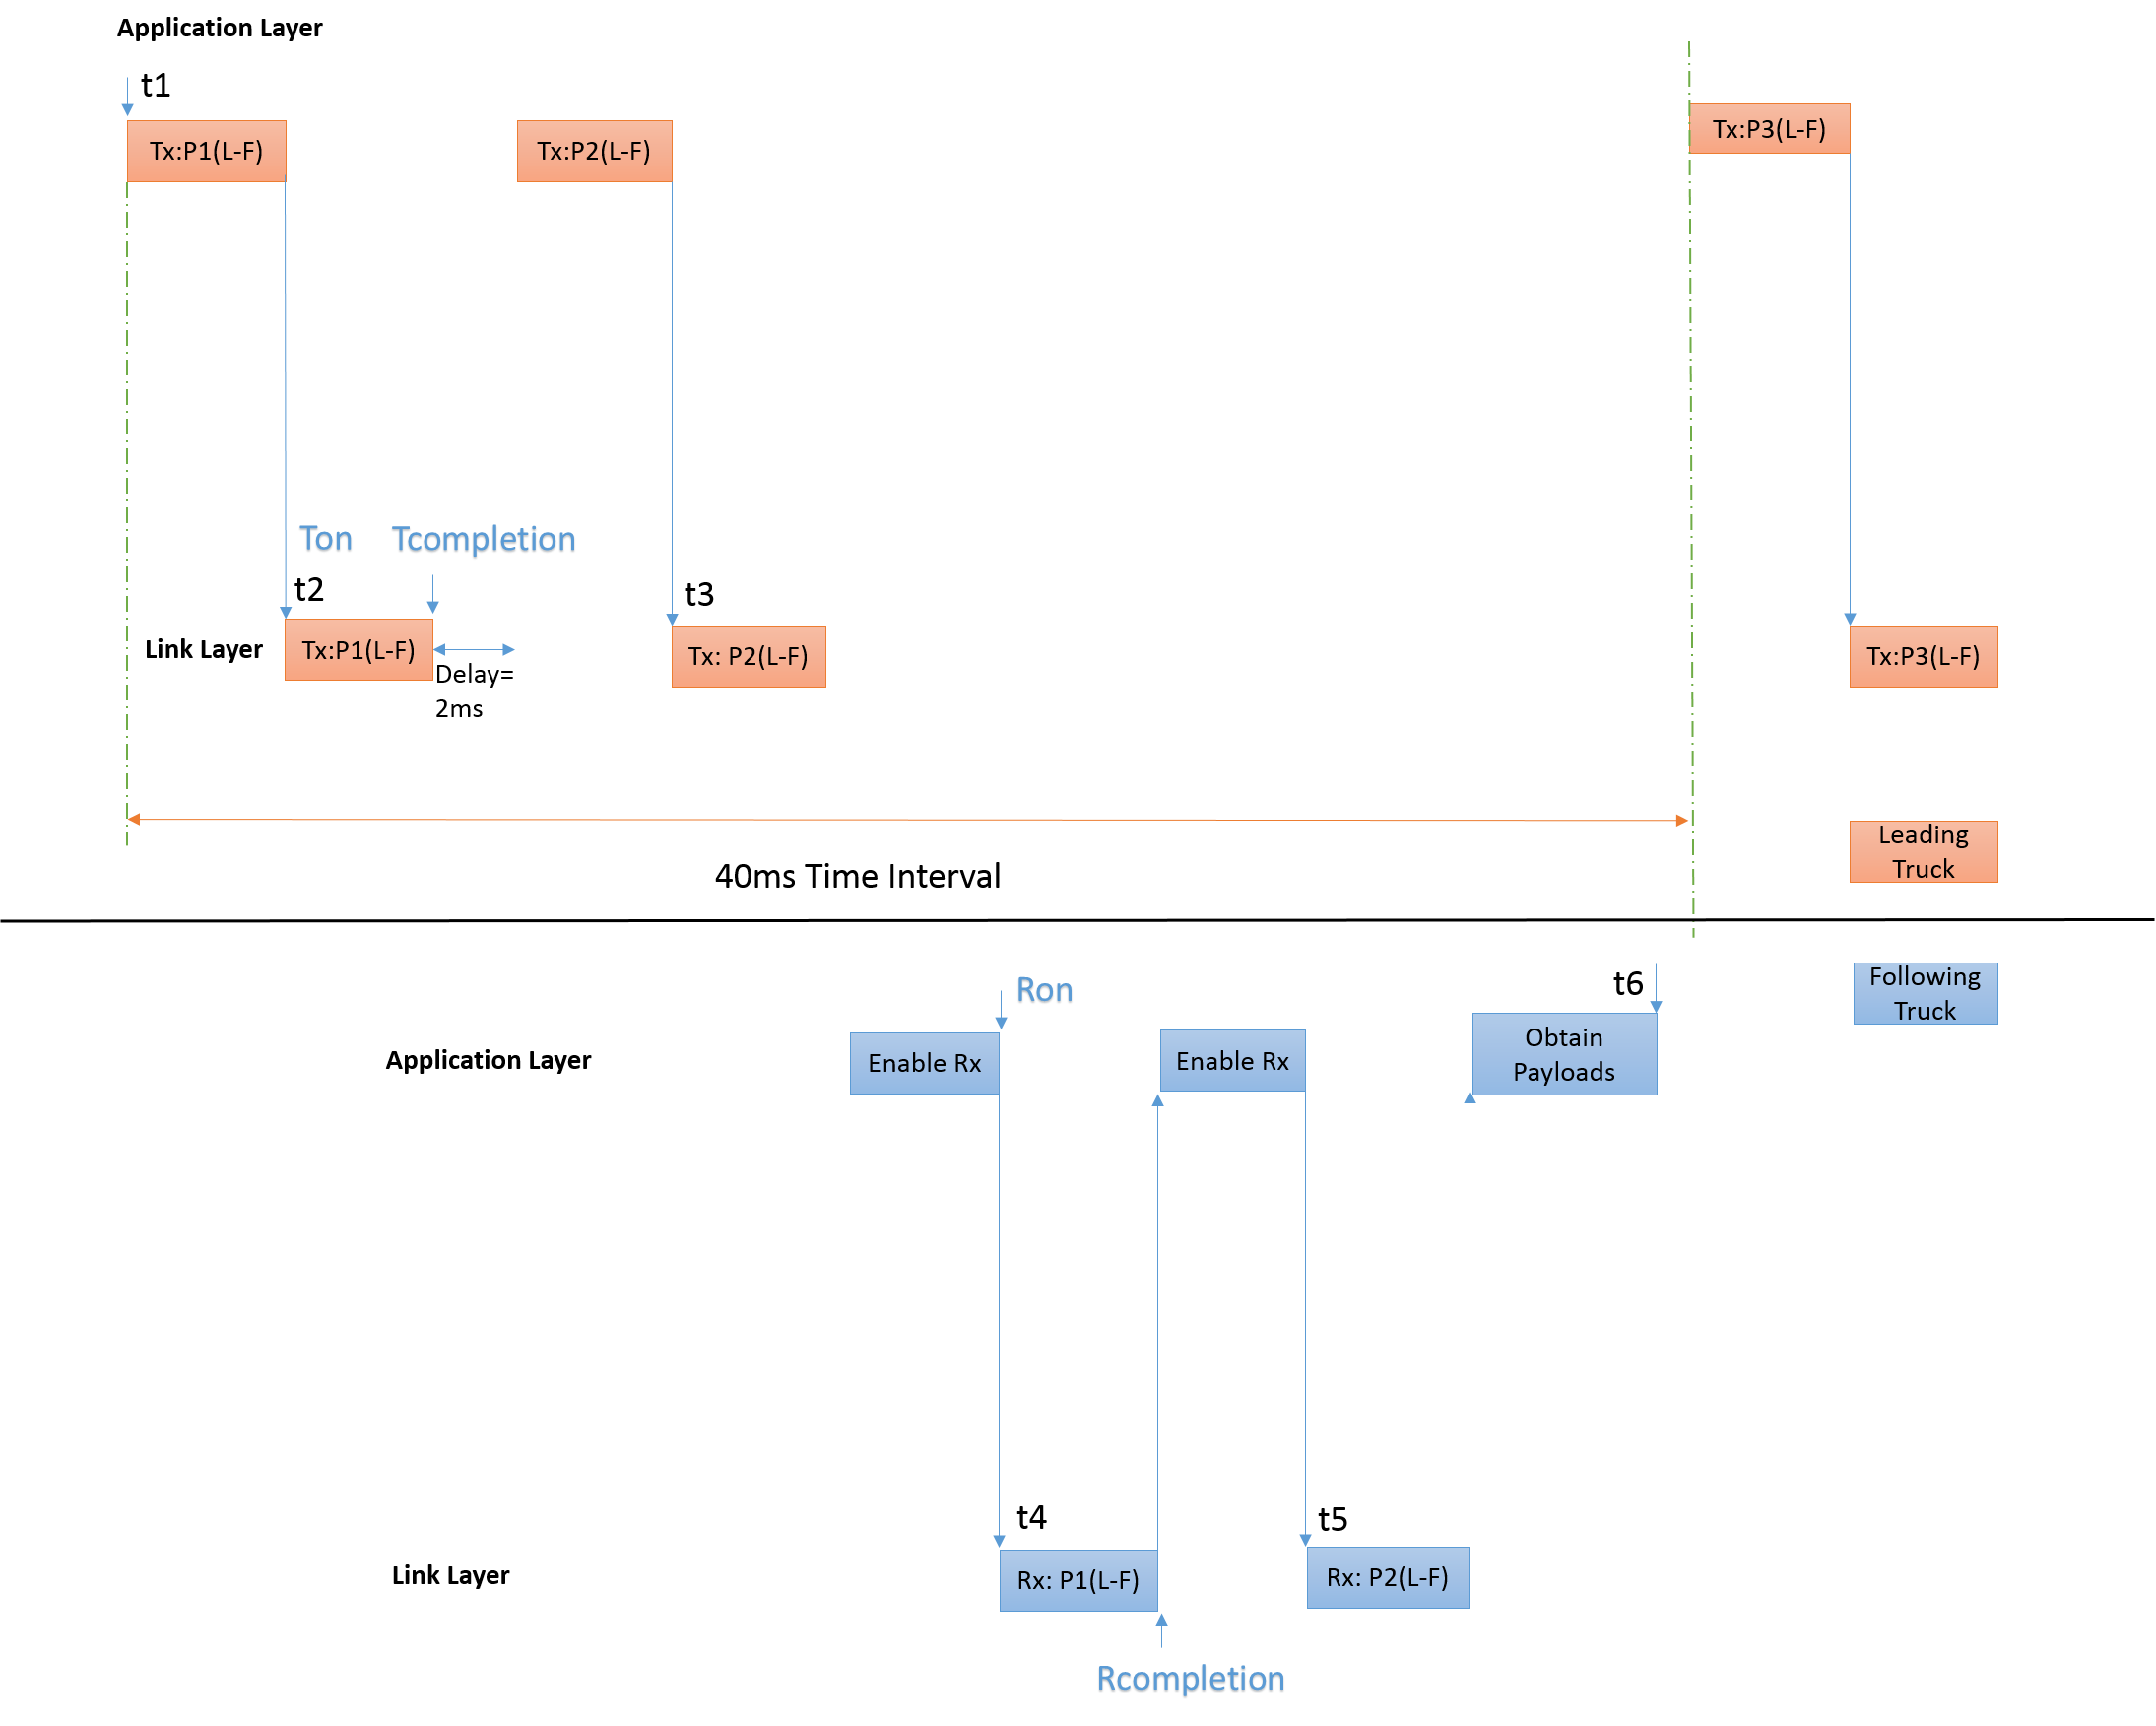
\includegraphics[width=1\textwidth]{figures/IndicationofLoggingParameters}
    \centering
    \caption{Logged parameters to determine appropriate working of the system}
    \label{fig:LoggedParametersDetermineAppWorking}    
\end{figure}




\subsection{MATLAB Implementation}
To process large data files created in the format as shown in Listing \ref{lst:loggingFormat}, we handle the log specific to each configuration at a time, on processing the log unique to that configuration completely; we go ahead with processing the log unique to the following configuration. Following this approach helps us to avoid storing significant amounts of data in memory which could lead to a MATLAB crash. On processing all the logs, we store the information appropriately so as to create desired graphs such as PER vs. Channel, MER vs. Channel, PER vs. Distance, Measured Distance vs. Calculated Distance, etc.

The parsing is implemented by obtaining the lines containing the string "messageLatency" from the log and stored in a cell array. A single row is created for each message with columns representing the parameter and its corresponding values. Depending on the number of messages and packets per message tested, appropriate number of lines are read that are specific to each configuration. The parameters packets per message, the number of messages, actual measured distance and the number of configurations tested and paths to the log files need to be input before running the post processing script.

The obtained cell array after parsing the log files is used for further processing. Based on the required results like PER, MER, message latency, packet latency, the accuracy of ranging, etc. the obtained cell array is traversed for the desired parameters and after applying the desired modifications on the data, it is stored in separate arrays corresponding to each result. Each row in these separate arrays corresponds to an average of all the values for the desired parameter in that specific configuration, and the column in these separate arrays corresponds to each run. It is to be noted that the cell array obtained by parsing the log files needs to be converted to numbers from strings to process them as indicated above. This process continues for all the configurations across all runs.

From these separate arrays, we obtain data and classify them based on channel, data rate, Preamble length, etc. by correlating with the configuration number. Consequently, the data is further processed based on the required result and the classification, and corresponding graphs created. The MATLAB implementation is such that it can process logs for up to four packets per message and any desired number of configurations and runs.

It is to be noted that based on the configurations that are tested, the code for classification needs to be modified because classification is performed by correlating with the configuration number. The MATLAB implementation currently calculates PER at leading truck, PER at following truck, MER at leading truck, MER at following truck, packet latency for leading truck (mean, min, max and standard deviation), packet latency for following truck (mean, min, max and standard deviation), message latency in leading truck (mean, min, max and standard deviation), message latency in following truck (mean, min, max and standard deviation), range accuracy, RX level at leading truck for each packet of a message (mean, min, max and standard deviation) and RX level at following truck for each packet of a message (mean, min, max and standard deviation). The MATLAB implementation allows creation of graphs with respect to the parameters stated above.
\clearemptydoublepage

\chapter{Duty Cycle Requirements for UWB}\label{chapter:dutycyclerequirements}
\nomenclature[A]{LDC}{Low Duty Cycle}
\nomenclature[A]{DAA}{Detect and Avoid}
\nomenclature[A]{EIRP}{Equivalent Isotropically Radiated Power}

In this chapter, we discuss the duty cycle requirements for UWB and determine if platooning application requirements meet the duty cycle requirements for UWB.

To permit the use of Ultra Wide Band (UWB) but mitigate the possibility/effect of interference with other systems, two main approaches have been adopted which include Low Duty Cycle (LDC), and Detect and Avoid (DAA). LDC in which UWB equipment must limit the relative time for which it is transmitting. Detect and Avoid (DAA) in which UWB systems listen for other UWB transmissions before they transmit. The LDC requirement needs to be met when using Band 3 of UWB wherein the center frequency is 4488 MHz. LDC and DAA requirements have to be met when using Band 1, Band 2 and Band 11 of UWB wherein the center frequencies are 3432 MHz, 3960 MHz, and 8712 MHz respectively as shown in Figure \ref{fig:UWBRegulations}. It is to be noted that Detect and Avoid is not supported by DecaWave DW1000, the hardware used for the implementation of the thesis. The channels supported by DecaWave DW1000 are as shown in the Figure \ref{fig:ChannelsDecawaveDW1000}.
From the Figure \ref{fig:UWBRegulations} and Figure \ref{fig:ChannelsDecawaveDW1000}, we can infer that LDC regulations need to be met when using Channels 1, 2, 3 and 4 of DecaWave DW1000, and the same is not required when operating in Channels 5 and 7.
\begin{figure}[htbp]
    \begin{center}
        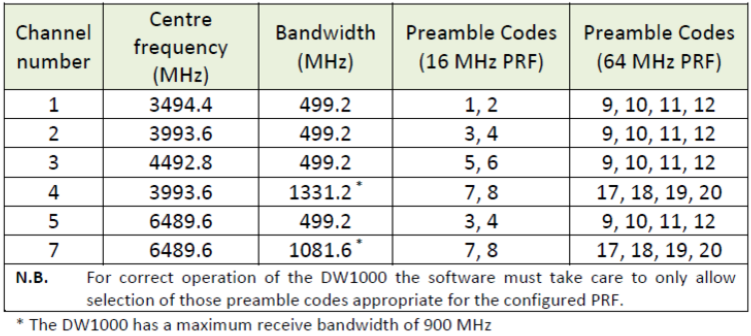
\includegraphics[width=1\textwidth]{figures/Picture2.png}
        \caption[Channels supported by DecaWave DW1000]{Channels supported by DecaWave DW1000 \protect\cite{DW1000UserManual}}
        \label{fig:ChannelsDecawaveDW1000}
    \end{center}
\end{figure}

\begin{figure}[htbp]
    \begin{center}
        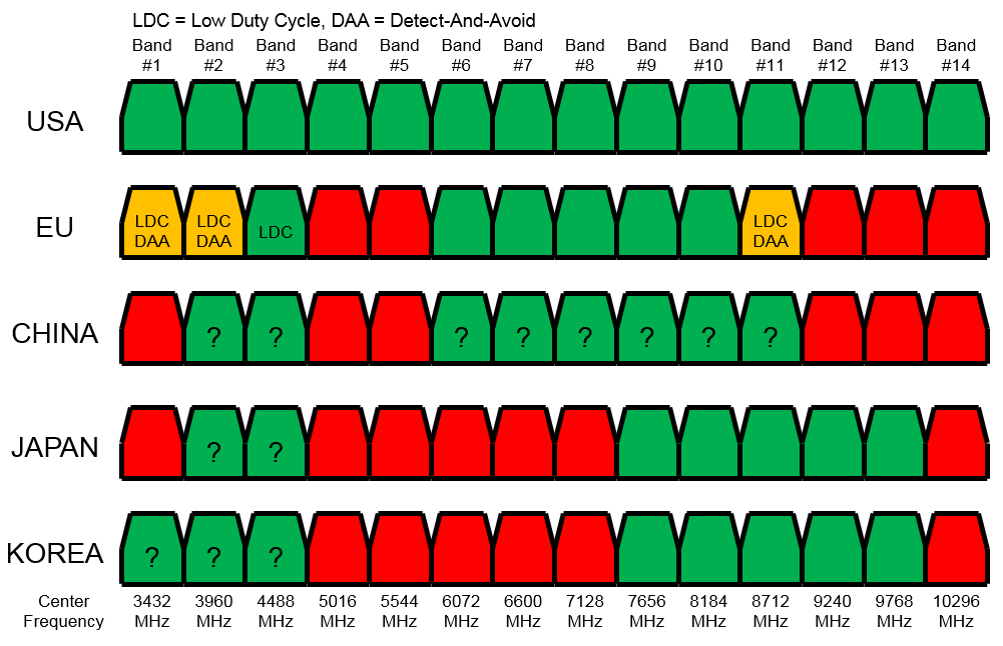
\includegraphics[width=1\textwidth, scale=0.7]{figures/Picture1.png}
        \caption{UWB Regulations, Source: F.Leong, NXP Semiconductors}
        \label{fig:UWBRegulations}
    \end{center}
\end{figure}

\section{Low Duty Cycle}
In Europe, the Electronic Communications Committee - one of CEPT's (European Conference of Postal and Telecommunications
Administrations) working committees dealing with radio spectrum use and telecommunications numbering\/ addressing, specifies technical requirements for LDC mitigation technique, enabling operation at -41.3 dBm /MHz Equivalent Isotropically Radiated Power (EIRP) within the band 3.4 - 4.8 GHz \cite{ECCDecision}. A device implementing LDC is a UWB device that meets the requirements as shown in Table ~\ref{fig:ECCDefLDC}.

\begin{table}[htbp]
    \begin{center}
        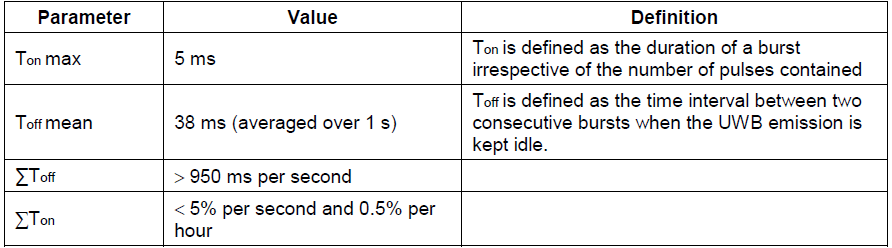
\includegraphics[width=1\textwidth]{figures/Picture3.png}
        \caption[ECC Definition of Low Duty Cycle Operation]{ECC Definition of Low Duty Cycle Operation \protect\cite{ECCDecision}}
        \label{fig:ECCDefLDC}
    \end{center}
\end{table}

To determine if LDC requirement can be met by truck platooning application, let's consider the UWB PHY frame structure and the application requirements.

\section{UWB PHY and Platooning Application}
UWB PHY frame structure is as shown in Figure \ref{fig:UWBPHYframeStructure}. According to the IEEE 802.15.4a UWB standard, the mandatory SHR Preamble base rate is 1.01 Msymbols/s and 0.25 Msymbol/s. The PHR is sent at 850 kb/s for all data rates greater than or equal to 850 kb/s and at 110 kb/s for the data rate of 110 kb/s.
The data field is transferred in MAC format as shown in Figure ~\ref{fig:MACMessageFormat} at the data rate defined experimentally. 

In truck platooning application, if we consider leading truck and the following truck, VFM (leading truck to the following truck) and PSM (following truck to the leading truck) are exchanged every 40 ms with a particular offset as shown in Figure \ref{fig:MessageExchangePlatooningApplication}.

Figure \ref{fig:DW1000SymbolDuration} shows the symbol durations for various configurations of PRF and data rate, which are used to calculate the LDC requirement for the truck platooning application.

\begin{figure}[htbp]
    \begin{center}
        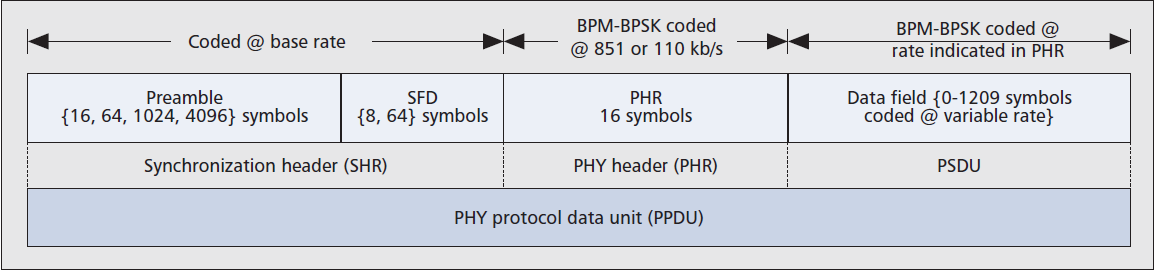
\includegraphics[width=1\textwidth]{figures/Picture4.png}
        \caption[UWB PHY Frame Structure]{UWB PHY Frame Structure \protect \cite{karapistoli2010overview}}
        \label{fig:UWBPHYframeStructure}
    \end{center}
\end{figure}

\begin{figure}[htbp]
    \begin{center}
        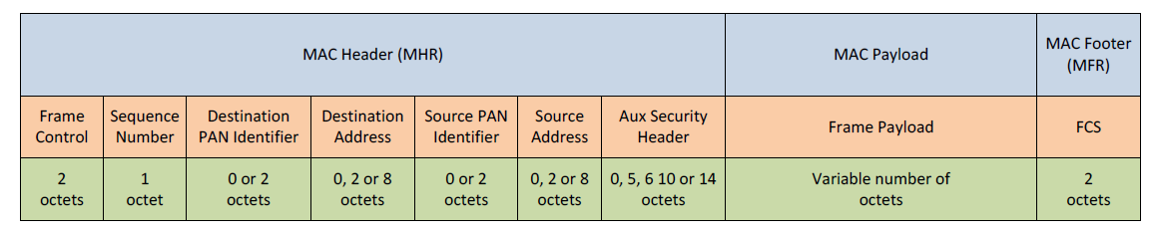
\includegraphics[width=1\textwidth]{figures/Picture5.png}
        \caption[802.15.4 - MAC Message Format]{802.15.4 - MAC Message Format \protect \cite{DW1000UserManual}}
        \label{fig:MACMessageFormat}
    \end{center}
\end{figure}

\begin{figure}[htbp]
    \begin{center}
        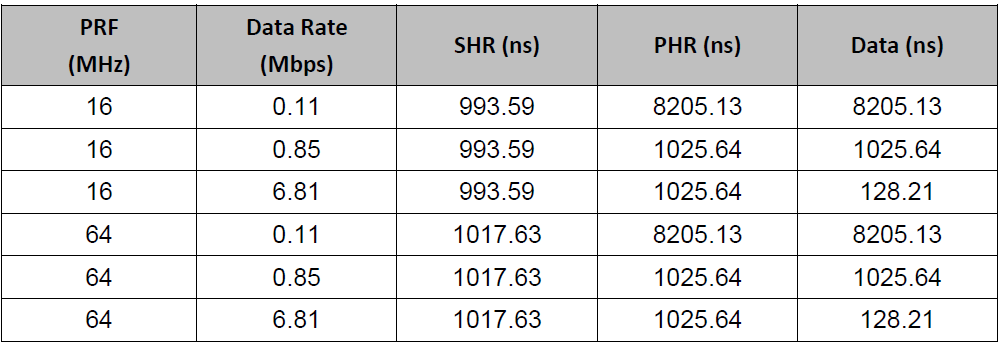
\includegraphics[width=1\textwidth]{figures/Picture7.png}
        \caption[DW1000 Symbol Durations]{DW1000 Symbol Durations \protect \cite{DW1000DataSheet}}
        \label{fig:DW1000SymbolDuration}
    \end{center}
\end{figure}

\section{LDC Calculation for the Truck Platooning Application}

According to the LDC requirement as specified in Table \ref{fig:ECCDefLDC}, the transmitter can be on for 50 ms of a second and 18000 ms of an hour. To check if the truck platooning application meets the LDC requirement, let's consider the typical platooning payloads of 60 bytes (1 packet/message) and 160 bytes (2 packets/message). Here, 60 bytes and 160 bytes corresponds to the minimum and maximum platooning payload of the current Eco-Twin Truck platooning implementation \cite{euTPC}.

For the calculation of the Ton times for 6.8 Mbps, following values are used for various parameters.
\vspace{0.2cm}
\\Preamble Length = 64 Symbols \\
Data Rate = 6.8 Mbps \\
Bit Rate = 6800 \\
PHR Rate = 850 \\
PHR = 19 bits \\
SFD length = 8 Symbols \\
PRF = 16 MHz (Symbol Duration = 993.59 ns) or 64 MHz(Symbol Duration = 1017.63 ns)\\

Let us calculate the respective Ton times for the following scenarios using Equation~\ref{eq:PreambleDuration} and Equation~\ref{eq:maxFrameDuration}. 
\begin{equation}
Preamble Duration = (preambleLength + sfdLength)* preambleSymbolDuration
\label{eq:PreambleDuration}
\end{equation}
\begin{equation}
maxFrameDuration = preambleDuration + 19/phrRate + packetSize * 8/ bitRate
\label{eq:maxFrameDuration}
\end{equation}

\begin{itemize}
    \item \textbf{Scenario 1: 60 bytes payload, 64 MHz PRF} For Scenario 1, we can determine that the maximum frame duration is 0.1662 ms. Considering a single mirror, 25  messages are transmitted in a second because of the platooning application requirement of 25 Hz. For 1 second, the total Ton time is 4.1550 ms out of the available 50 ms and for 1 hour, the total Ton time is 14958 ms out of the available 18000 ms. Since the max duration of a burst is always less than 5 ms. LDC requirement is met in this scenario. 
    
    \item \textbf{Scenario 2: 60 bytes payload, 16 MHz PRF} For Scenario 2, we can determine that the maximum frame duration is 0.1645 ms. For 1 second, the total Ton time is 4.1125 ms out of the available 50 ms and for 1 hour, the total Ton time is 14805 ms out of the available 18000 ms. Since the max duration of a burst is always less than 5 ms. LDC requirement is met in this scenario too. 
    
    \item \textbf{Scenario 3: 160 bytes payload, 64 MHz PRF} For Scenario 3, we can determine that the maximum frame duration is 0.3794 ms if we transmit two packets each of 80 bytes. For 1 second, the total Ton time is 9.4850 ms out of the available 50 ms and for 1 hour, the total Ton time is 34146 ms out of the available 18000 ms. LDC requirement is not met in this scenario because of the hourly constraint. 
    
    \item \textbf{Scenario 4: 160 bytes payload, 16 MHz PRF} For Scenario 4, we can determine that the maximum frame duration is 0.3760 ms if we transmit two packets each of 80 bytes. For 1 second, the total Ton time is 9.4000 ms out of the available 50 ms and for 1 hour, the total Ton time is 33840 ms out of the available 18000 ms. LDC requirement is not met in this scenario because of the hourly constraint. 
    
\end{itemize}

Hence the UWB system for truck platooning will meet the LDC requirement according to the regulations when 6.8 Mbps data rate, 60 bytes minimum platooning payload, minimum preamble length, and a UWB transceiver mounted on a single mirror is considered. 

\vspace{3cm}
Similarly, we can calculate Ton times for 850 Kbps and 110 Kbps using Equation~\ref{eq:PreambleDuration} and Equation~\ref{eq:maxFrameDuration}. For the calculation of Ton times for 850 Kbps, following values are used for various parameters.
\vspace{0.2cm}
\\Preamble Length = 256 Symbols \\
Data Rate = 850 Kbps \\
Bit Rate = 850 \\
PHR Rate = 850 \\
PHR = 19 bits \\
SFD length = 8 Symbols \\
PRF = 16 MHz (Symbol Duration = 993.59 ns) or 64 MHz(Symbol Duration = 1017.63 ns)\\

For the calculation of Ton times for 110 Kbps, following values are used for various parameters.
\vspace{0.1cm}
\\Preamble Length = 2046 Symbols \\
Data Rate = 110 Kbps \\
Bit Rate = 110 \\
PHR Rate = 110 \\
PHR = 19 bits \\
SFD length = 8 Symbols \\
PRF = 16 MHz (Symbol Duration = 993.59 ns) or 64 MHz(Symbol Duration = 1017.63 ns)\\


% Please add the following required packages to your document preamble:
% \usepackage{multirow}
% \usepackage{graphicx}
\begin{table}[]
    \centering
    \caption{Ton with respect to data rates for Platooning application}
    \label{tab:Ton with respect to data rates for Platooning application}
    \resizebox{\textwidth}{!}{%
        \begin{tabular}{|l|c|c|c|c|}
            \hline
            \multirow{2}{*}{\textbf{Data Rate}} & \multicolumn{4}{c|}{\textbf{Ton Duration in milliseconds (calculated per hour)}}                                                                                                                                    \\ \cline{2-5} 
            & \multicolumn{1}{l|}{\textbf{60 bytes, 64 MHz PRF}} & \multicolumn{1}{l|}{\textbf{60 bytes, 16 MHz PRF}} & \multicolumn{1}{l|}{\textbf{160 bytes, 64 MHz PRF}} & \multicolumn{1}{l|}{\textbf{160 bytes, 16 MHz PRF}} \\ \hline
            \textbf{6.8 Mbps}                   & 14958                                              & 14805                                              & 34146                                               & 33840                                               \\ \hline
            \textbf{850 Kbps}                   & 77013                                              & 76446                                              & 187902                                              & 186768                                              \\ \hline
            \textbf{110 Kbps}                   & 601704                                             & 597132                                             & 1465218                                             & 1456092                                             \\ \hline
        \end{tabular}%
    }
\end{table}

Table \ref{tab:Ton with respect to data rates for Platooning application} summarizes the Ton durations with respect to data rates 6.8 Mbps, 850 Kbps and 110 Kbps for Platooning application. It is to be noted that the LDC requirement is not fulfilled for all scenarios when 850 Kbps or 110 Kbps is used because, for 1 hour, the total Ton time must be within 18000 ms. Only in the case of 6.8 Mbps, LDC requirement is met when 60 bytes minimum platooning payload, minimum preamble length and a UWB transceiver mounted on a single mirror is considered. 
\clearemptydoublepage


\chapter{Experiments and Results}\label{chapter:experimentsAndResults}
Content is not included for reasons of confidentiality.
\clearemptydoublepage

\chapter{Conclusion and Future work}\label{chapter:conclusionAndFutureWork}
Content is not included for reasons of confidentiality.
\clearemptydoublepage







%\chapter{Literature Review}\label{chapter:Literature_review}
%This chapter contains a brief literature survey about design methodology of tubular receivers implemented by several researchers. An overview of the design criteria and the existing heat transfer models of tubular receivers available in the literature are also discussed.

\section{Tubular Receivers}
Tubular receivers are the most widely used state of the art receiver technology \cite{Goswami.2007}. There are four common system options available based on the receiver and storage fluid. The first two are state of the art systems and the other two are still in research phase.
\begin{figure}[h!]
	\includegraphics[width=0.5\textwidth]{figures/tubular_receiver_cavity_external}
	\centering
	\caption{Tubular receivers \cite{Wagner.2008}}
\end{figure}
\subsection{Water/Steam} 
\begin{figure}[h!]
	\includegraphics[width=0.5\textwidth]{figures/water_steam}
	\centering
	\caption{Flow layout of water/steam central receiver system \cite{water_steam}}
\end{figure}
In this type of system, water is used as a heat transfer fluid (HTF) and so there is a direct steam generation in the receiver itself. One of the main advantages of this system is no need of heat exchanger if storage is not considered. But, the disadvantages of this system are
\begin{itemize}
\item Low receiver peak flux limit (0.3 to 0.6 $MW/m^2$) \cite{Falcone.1986}.
\item  Storing energy in the form of high-pressure steam is uneconomical and so the energy must be transferred to some other medium with heat exchangers resulting into higher energy loss.
\item  Two-phase heat transfer in the receiver directly influences its design.
\item  The pioneer CSP power plant, solar one used oil/rock thermocline storage. The maximum temperature limitation of oil is 315 $^{\circ}$C and so the output steam from the storage has low temperature which results in the low turbine gross efficiency \cite{Falcone.1986}.
\end{itemize}
\subsection{Molten Salt}
\noindent Molten salt is an attractive HTF for CSP plants with storage because of its low cost and its commercial availability. Some of the attractive features \cite{Falcone.1986} are
\begin{figure}[h!]
	\includegraphics[width=0.7\textwidth]{figures/molten_salt_layout}
	\centering
	\caption{Flow layout of molten salt central receiver system \cite{Wagner.2008}}
\end{figure}
\begin{itemize}
\item High receiver peak flux limit compared to water/steam system (0.6 to 0.8 $MW/m^2$).
\item State of the art technology with 40 years of operational experience as an HTF. 
\item Non-toxic and stable over an extended period of time when protected from the environment and overheating. 
\item Molten salt is 2 to 3 times cheaper than sodium.
\end{itemize}
\subsection{Liquid Sodium}
\begin{figure}[h!]
	\includegraphics[width=0.5\textwidth]{figures/sodium_htf}
	\centering
	\caption{Flow layout of liquid sodium central receiver system \cite{Falcone.1986}}
\end{figure}
Liquid sodium has very good heat transfer properties and so it has low thermal losses due to the reduced area of the receiver. Mostly, sodium receivers are external type with already reduced losses and so the further loss reduction with cavity type receiver is not shown to be beneficial \cite{Falcone.1986}. Compared to molten salt, liquid sodium has very good heat transfer properties \cite{Falcone.1986} which are given below:
\begin{itemize}
\item Receiver peak flux limit (in excess of 1.5 $MW/m^2$).
\item Higher thermal conductivity and so it is able to operate with high incident solar flux.
\item Sodium has five times higher heat transfer rate than molten salt and so single pass is enough in the receiver fluid flow.
\item Sodium freezes at 100 $^{\circ}$C which is two times lower when compared with molten salt.
\item Sodium has higher boiling point (873 $^{\circ}$C) \cite{Nicholas.2012} which allows it to operate in other high-temperature cycles also.
\item Because of the higher operational flux, receiver size, cost and its losses are reduced resulting into higher receiver efficiency.
But, there are many limiting factors which act as a hindrance for sodium receiver to be commercially accomplished. Some of them \cite{Falcone.1986} are stated below:
\item The relatively high cost and low specific heat of sodium limit its usage as sensible heat storage medium.
\item Low volumetric heat capacity of sodium makes the storage tank larger and costlier.
\item The main point to note is that the highly reactive nature of sodium and water has to be considered while designing.
\end{itemize}
\subsection{Sodium/Salt Binary}
\begin{figure}[h!]
	\includegraphics[width=0.5\textwidth]{figures/sodium_binary_htf}
	\centering
	\caption{Flow layout of sodium/salt binary central receiver system \cite{Falcone.1986}}
\end{figure}
\noindent The fourth option, in which sodium is used as a receiver fluid and molten salt is used as the storage fluid. It combines the attractive feature of both fluids but the additional heat transfer loop is needed to couple the system to run which adds complexity. The risk of sodium fire is reduced because it is restricted within the concrete tower but the reaction between sodium and molten salt is not well-known. Current indications are that it would be strongly exothermic and release the gaseous product which may cause pressurisation problem \cite{Falcone.1986}.

\section{Receiver Design Methodology}
This section summarises the receiver design methodology suggested by various researchers.

\subsection{Falcone [1986] \cite{Falcone.1986}}
Falcone \cite{Falcone.1986} suggested the following steps for the tubular receiver design: 
\begin{enumerate}
	\item Calculate the thermal rating of the receiver based on system level requirements like plant output, type of receiver fluid and storage media, nature of power cycle and solar multiple.
	\item Select the flux limit based on working fluid and the tube material of the receiver.
	\item Then, calculate the required receiver absorber area for the given allowable flux limit.
	\item The receiver size should be within the limit of practical size.
	\item The minimum receiver size is largely a function of spillage considerations based on the size of reflected heliostat beam and the size of its target. The beam size increases along with the size of heliostat even for the focused and canted mirrors. The receiver size also corresponds to reflected beam size in order to keep the spillage losses within a reasonable limit.
	\item The maximum practical size is limited by the height of receiver panels due to shipping constraints.
\end{enumerate}
\subsection{Zavoico [2001] \cite{Zavoico.2001}}
Zavoico \cite{Zavoico.2001} suggested the following steps for the tubular receiver design: 
\begin{enumerate}
	\item Establish the allowable incident flux as a function of bulk salt temperature, allowable cumulative tube strains and corrosion rates at the salt film temperature.
	\item Estimate the receiver size based on the maximum allowable flux.
	\item Estimate the heat losses for various combinations of receiver height and diameter. 
	\item Then, the aspect ratio should be selected for the maximum receiver efficiency.
	\item The dimensions of the receiver should be selected such that it gives the lower cost.
\end{enumerate}
\subsection{Lata [2008] \cite{Lata.2008}}
Lata \cite{Lata.2008} tried to optimize the receiver dimensions in order to increase the allowable peak flux of molten salt receiver from 0.85 $MW/m^2$ to 1 $MW/m^2$. Basically, their design methodology is similar to other researchers. In addition, they tried to optimise the following receiver dimensions.
\begin{enumerate}
	\item Receiver size optimisation to minimise the thermal losses (H/D ratio selection).
	\item Small fluid cavity to maximise the receiver thermal efficiency and to prevent fatigue-creep damage (Tube diameter selection).
	\item Thin walled conduction to improve thermal efficiency (Tube wall thickness selection).
	\item Minimise the pressure losses by optimising the number of panels and molten salt circuit routeing (Number of panels and fluid path selection).
	\item High nickel alloy material with excellent mechanical properties (Material selection).
\end{enumerate}
All the above said design criteria for the receiver will be discussed in the next section.
\subsection{System Advisory Model (SAM) \cite{Wagner.2008}}
The performance model of SAM uses the TRNSYS components developed at the University of Wisconsin and the solar field optimisation algorithm is based on the DELSOL3 model developed at the Sandia national laboratory. It is capable of operating in two modes. The first one calculates the performance of an existing system. The second one is an optimisation of system design. \\\\
In the optimisation process, the tower height and receiver sizes are iteratively evaluated to find out the minimum possible cost of electricity output. But, the optimisation process needs the initial guess defined by the user. Then, the guess value is iteratively evaluated within the range given below. One of the limitation is that the educated guess of tower height has to be supplied by the user. It may mislead into wrong results if the guess value is not appropriate. The following are the ranges for the different parameters used for the optimisation.
\nomenclature[S]{P}{Power \nomunit{W}}
\nomenclature[S]{H}{Height \nomunit{m}}
\nomenclature[S]{D}{Diameter \nomunit{m}}
\nomenclature[Z]{el}{Electric}
\begin{itemize}
	\item Nominal plant electric output power: $ \quad  \frac{1}{2}P_{el,guess}\le P_{el,guess} \le 5 \times P_{el,guess} $
	\item Tower height: $ \quad  0.6 \times H_{tower} \le H_{tower} \le 2 \times H_{tower} $
	\item Receiver Diameter: $ \quad  0.4 \times D_{rec}\le D_{rec} \le 1.8 \times D_{rec} $
	\item Height to Diameter ratio (Aspect ratio): $ \quad 0.6 \times \frac{H_{rec}}{D_{rec}}\le \frac{H_{rec}}{D_{rec}} \le 1.4 \times \frac{H_{rec}}{D_{rec}} $ 
\end{itemize}
They have developed objective function for the minimisation of the lowest energy cost and optimising iteratively based on the objective function by varying all the parameters within this range.

\section{Design Criteria}
The design criteria summarise about every parameter which needs to be optimised for better receiver design.
\subsection{Allowable Peak Flux Limit }
\begin{figure}[h]
	\includegraphics[width=0.5\textwidth]{figures/Receiver_flux_graph}
	\centering
	\caption{Receiver peak flux value for different HTF and materials with respect to life cycles \cite{Falcone.1986}}
\end{figure}
The normal range of flux limit for the receiver fluids is tabulated below.
\begin{table}[h]
\begin{center}
	\begin{tabular}{ |c|c|c|c| } 
		\hline
		 \textbf{Name of the HTF} & \textbf{Flux limit range} & \textbf{Unit} \\
		\hline
		Water/Steam & 0.3 to 0.6 & $ MW/m^2 $ \\ 
		\hline
		Molten Salt& 0.6 to 0.85 & $ MW/m^2 $ \\ 
		\hline
		Liquid Sodium& 1.2 to 1.3 & $ MW/m^2 $ \\ 
		\hline
	\end{tabular}
	\caption{Receiver flux limit for different HTF\label{Receiver_flux_limit} \cite{Falcone.1986}}
\end{center}
\end{table}
It is based on the tube material and with the required number of life cycles. \figurename{ 2.6} represents the graph of receiver peak flux for different HTF and materials \cite{Falcone.1986}. In the graph, allowable flux limit of molten salt and sodium receiver with two types of steel are plotted with respect to life cycles. As a goal of 30 years lifetime for the receiver, it would be roughly 11000 cycles at the rate of one cycle per day. But, one should take into account for the transients due to weather conditions also. The allowable peak flux, ${q_o}$ can be calculated based on the simple model using the allowable thermal strain, thermal expansion and the poisson ratio of the material \cite{Liao.2014}. The average flux can be calculated by peak to average flux ratio. According to Stine and Harrigan \cite{Stine.1985}, the peak to average flux ratio can be between 2 to 3.
\nomenclature[G]{$\varepsilon$}{Allowable strain of the material \nomunit{-}}
\nomenclature[G]{$\delta$}{Thermal expansion coefficient \nomunit{1/m K}}
\nomenclature[G]{$\upsilon$}{ Poisson's ratio \nomunit{-}}
\nomenclature[S]{k}{Thermal conductivity \nomunit{W/m K}}
\nomenclature[S]{d}{Diameter of the receiver tube \nomunit{m}}
\nomenclature[S]{h}{Heat transfer coefficient \nomunit{W/m$^2$ K}}
\nomenclature[S]{R}{Thermal Resistance \nomunit{K/W}}
\nomenclature[S]{q$_o$}{Allowable peak flux \nomunit{W/m$^2$}}
\nomenclature[Z]{cond}{Conduction}
\nomenclature[Z]{o}{Outer}
\nomenclature[Z]{i}{Inner}
\begin{equation}
{q_o} = \frac{\varepsilon} {\delta [\frac{2}{1-\upsilon}R_{cond} + \frac{\pi}{\pi -1} (\frac{1}{2}R_{cond} + R_{conv})]}
\end{equation}
where
\begin{itemize}
	\item $R_{cond} = \frac{d_o}{2k_m}ln(\frac{d_o}{d_i})$
	\item $R_{conv} = \frac{d_o}{d_i} \frac{1}{h}$
	\item $\varepsilon$ = Allowable strain of the material
	\item $\delta$ = Thermal expansion coefficient, 1/m K
	\item $\upsilon$ = Poisson's ratio
	\item R = Thermal resistance, K/W
	\item d = Diameter of the receiver tube, m
	\item k = Thermal conductivity of the material, W/m K
	\item h = Heat transfer coefficient, W/m$^2$ K
	\end{itemize}
\subsection{Receiver Sizing}
Incident receiver thermal power should be estimated in order to size the receiver. Then, the allowable peak flux should be decided to calculate the absorber area required to handle the flux. The selection of the allowable peak flux has to be done carefully to avoid any failure. Generally, one-half to one-third of the peak flux \cite{Stine.1985} is selected as an average flux and the receiver is sized for the average flux in order to ensure that it would not fail. \\\\
For cavity receivers, the inner surfaces of the receiver are exposed to re-radiation because of the enclosed structure and it may lead to overheating. According to Falcone \cite{Falcone.1986}, the receiver size for cavity receivers is 25 percent larger than the external receiver for the same incident receiver thermal power. So, the average flux can be selected accordingly for the cavity receivers in order to ensure that it would not fail. Then, the receiver geometry is designed with the aim of lower cost and higher efficiency. The following section explains how to design the receiver geometry.
\subsection{Receiver Aspect Ratio}
According to the statement of Falcone \cite{Falcone.1986}, the receiver aspect ratio (height to diameter ratio) would be between 1 to 2. But, it should be optimised for minimum thermal losses and trade-off with spillage loss should also be considered. According to the statement of Zavoico \cite{Zavoico.2001}, the receiver aspect ratio will be in the range of 1.2 to 1.5 but it should be selected for maximum receiver efficiency. For cavity receivers, it is known as height to width ratio which is usually in the range of 0.7 to 1 \cite{Falcone.1986}. Some of the other design considerations from literatures \cite{Falcone.1986} \cite{Zavoico.2001} are:
\begin{itemize}
	\item  The shipping constraint of the sub-assembly of panel tubes and the maximum continuous length of available seamless tubing limit the receiver height to 30m. But currently, there are some power plants which slightly crossed this limit. Crescent Dunes Solar Energy Project in US has the receiver height of 30.48 m \cite{Crescent} and the Atacama-1 project in Chile has been planned for the receiver height of 32 m \cite{Atacama}. 
	\item The larger height is desirable because of the high pointing accuracy of the heliostats (low spillage loss). 
	\item The larger diameter is desirable to maximise the interior space available to place all the receiver components but resulting into increased thermal losses due to the larger diameter. So, space allocation design analysis should also be considered to optimise the aspect ratio.
\end{itemize} 
\subsection{Tube Diameter Selection}
The receiver tube diameter can vary between 20 mm to 45 mm \cite{Lata.2008} and generally made of stainless steel or Incoloy. The analysis by Lata \cite{Lata.2008} states the following: 
\begin{itemize}
	\item Smaller the diameter, higher the receiver efficiency because it increases the salt velocity which in turn increases the heat transfer coefficient. But, the limitation of smaller diameter is that it increases the manufacturing cost and also the pressure drop due to the increased number of tubes.
	\item Pressure drop is directly proportional to the length of the salt circuit and to the square of the salt velocity and it is inversely proportional to the tube diameter. So, tradeoff between pressure drop and receiver efficiency should be done to optimise the tube diameter.
	\item Smaller the tube wall thickness, higher the heat transfer rates because it reduces the temperature gradients and therefore the efficiency is increased. But, the practical constraint is that the wall thickness is limited to commercial values.
\end{itemize}
\subsection{Fluid Flow Path Selection}
\begin{figure}[h]
	\includegraphics[width=0.7\textwidth]{figures/flow_config}
	\centering
	\caption{Eight possible fluid flow configuration by Wagner \cite{Wagner.2008}}	
\end{figure}
\noindent The fluid flow path is one of the main design considerations in order to avoid the uneven distribution of heat flux. Falcone \cite{Falcone.1986} states that the upward fluid flow is preferable so that the buoyancy force of warmer does not counteract the pumping pressure. But for the molten salt receiver, multi-pass flow is needed and so it is difficult to design the upward fluid flow configuration in all the tubes. So, serpentine flow (up and down) is one of the best flow configurations. Wagner \cite{Wagner.2008} developed a receiver model to analyse the behaviour of the solar power plants and he studied eight possible fluid flow configuration of the receiver. The following suggestions are given by Wagner \cite{Wagner.2008} to design the efficient receiver:
\begin{itemize}
	\item It is observed that the configuration with single flow path has higher pressure drop and so the parasitic pump power is increased. Hence, the two parallel flow path in the receiver is suggested in order to obtain the higher receiver thermal efficiency. 
	\item In Northern hemisphere, the south to north flow configuration gives higher efficiency because if cold fluid enters the higher flux panel in northern side, it will lead to higher thermal losses. 
	\item During peak flux, the hot fluid from the south side could not be able to cool the higher flux northern panel. So, the northern panels are exposed to higher thermal stresses during peak hours which is not recommendable.
	\item Hence, in the Northern hemisphere, the north to south flow configuration with two parallel flow path with or without a crossover is recommended for higher efficiency with low thermal stress.
\end{itemize}
Rodriguez-Sanchez \cite{Rodriguez.2015} simulated the same eight flow configurations to select the best with the aim of increasing the receiver availability and the global efficiency of the solar tower plant. He also obtained the similar results like Wagner and he proposed that the north to south flow configuration with one crossover in the middle is the best configuration based on the considerations of receiver thermal efficiency, distributed flux, tube temperature and the thermal stress.
\subsection{Tower Sizing}
The tower height is mainly a function of the receiver thermal power of the plant \cite{Falcone.1986}. The tower height is also influenced by the type of solar field. Falcone \cite{Falcone.1986} presented the graph which shows the range of tower height for the given receiver thermal power and the type of solar field. The towers can be built of steel or concrete. Steel tower will look like wired microwave relay towers and the concrete tower will be similar to chimneys at industrial plants \cite{Falcone.1986}. \figurename{ 2.8} shows both steel and concrete type tower. The choice of selecting the type of tower mainly depends on the height of the tower \cite{Falcone.1986}. The steel tower is shown to be beneficial below 120 m  and concrete tower will be preferred for height more than 120 m \cite{Falcone.1986}. The cost of tower increases with increasing tower height. 
\begin{figure}[h]
	\includegraphics[width=0.7\textwidth]{figures/tower_sizing_pic}
	\centering
	\caption{Solar tower for external and cavity receivers \cite{Feierabend.2010}}
\end{figure}
\section{Cavity Specific Design Criteria}
The following section consists of design criteria specific for cavity receivers. There is no specific design criteria needed for external receivers. 
\subsection{Cavity Receiver Geometry}
The cavity receiver geometry is designed to reduce thermal losses by enclosing the absorber tubes inside the cavity. The receiver aspect ratio acts as a primary design parameter for the cavity receiver geometry which is generally 0.7 to 1 \cite{Falcone.1986}. It decides the width and height of the aperture opening and the radius of the cavity. In the cavity receiver, all the piping and headers are placed inside the cavity and so there is some space needed on the top and bottom of the absorber tubes. It should be considered while designing the cavity receiver geometry. Generally, these spaces are covered by the lip to avoid heat losses. The design of lip is explained in the subsection lip height. Like active surfaces, the inactive surfaces are also heated up due to re-radiation and so careful selection of receiver allowable flux is necessary. 
\begin{figure}[h]
	\includegraphics[width=0.7\textwidth]{figures/cavity_receiver_geometry}
	\centering
	\caption{Cavity receiver with three of four receiver panels assembled in PS10 power plant \cite{Feierabend.2010}}
\end{figure}
\subsection{Cavity Opening Angle}
The cavity opening angle is the coverage angle of the radiation to the receiver from the solar field. Usually, the cavity opening angle is 180 degrees and the commercial plants like PS 10 are designed with the cavity opening angle of 180 degrees \cite{Feierabend.2010}. But, it actually depends on the solar field arrangement. Lukas \cite{Feierabend.2010} calculated the receiver thermal efficiency with the various cavity opening angle. He observed that the receiver thermal efficiency increases with the increasing cavity opening angle. It is explained that because of the decrease in aperture opening, heat loss will be lowered which in turn results in higher efficiency. But, it is not possible to distribute the heat flux uniformly for the higher cavity opening angle and so it can't be applied in real applications \cite{Feierabend.2010}.
\subsection{Lip Height (Aperture to Total Height Ratio) } 
The lip height which is usually specified as the aperture to total height ratio. The difference between the total height to aperture height is known as lip height. Generally, the upper lip reduces the heat losses and the lower lip does not have much effect on the heat losses \cite{Kraabel.1983}. The value of aperture to total height ratio used by Lukas is 0.75 \cite{Feierabend.2010}. If the aperture to total height ratio is further increased, it will decrease the heat loss but the spillage loss is increased. Hence, the tradeoff should be done in order to optimise the aperture to total height ratio.
\subsection{Cavity Inclination}
\begin{figure}[h]
	\includegraphics[width=0.3\textwidth]{figures/cavity_inclination}
	\centering
	\caption{Cavity inclination angle \cite{Ma.1993}}	
\end{figure}
The cavity inclination can vary from 0${^\circ}$ to 90${^\circ}$. The convective heat loss of the cavity receiver depends on the wind speed, wind direction and also depends on the cavity inclination. Flesch \cite{Flesch.2015} conducted the cryogenic wind tunnel experiment and observed the influence of wind on the convective loss for head on and side on wind direction. In the no wind condition, the convective heat loss decreases with increasing receiver tilt angle\cite{Clausing.1981} \cite{Clausing.1983}. But with higher wind speed, the higher tilt angle also contributes to higher losses. From the analysis of cryogenic wind tunnel experiment, Flesch \cite{Flesch.2015} observed that the cavities should be designed in such a way that the wind flow is parallel to the aperture plane so that there is lesser wind influence to the heat losses. Moreover, cavity inclination is recommended in order to reduce the convection losses \cite{Flesch.2015}. 
\section{Heat Transfer Model}
The heat loss model which consists of heat loss due to external convection, radiation and reflection. Conduction loss to the back side of the receiver panel is small compared to other losses \cite{Stine.1985} and so it is neglected in this study. The overview of various heat transfer models is summarised in this section. It is divided into two subsections as external and cavity receivers. 
\subsection{External Receiver}
In the external receiver, the entire absorber area is exposed to the surroundings. So, there are higher thermal losses from the receiver to the surroundings when compared to cavity receivers. The main thermal losses include convection and radiation heat loss.
\subsubsection{Convective Heat Loss}
The heat transfer equations for the convection heat loss of cylindrical receivers are same like basic textbook equations. But, the Nusselt correlation that can be applied to the large-scale receivers is the ambiguous area in which a lot of researches are carried out \cite{Siebers.1984} \cite{Cengel.2003}. For the cylindrical receivers, heat transfer has an influence of both natural and the forced convection and so the mixed convection is usually considered \cite{Siebers.1984}. In order to find out which heat transfer is dominant, Richardson number is used \cite{Teichel.2011} and it is explained in the next subsection.\\\\
According to literatures \cite{Cengel.2003} \cite{Siebers.1984}, heat transfer coefficient for mixed convection, $h_{mix}$ can be stated with the following correlation. According to Cengel \cite{Cengel.2003}, the value $m$ lies between 3 and 4. The value close to 3 suits better for vertical surfaces and the larger values are suited for horizontal surfaces. Siebers \cite{Siebers.1984} studied this value particularly for both receivers and estimated the best-suited value of 3.2 and 1 for external and cavity receiver respectively.
\nomenclature[Z]{nat}{Natural}
\nomenclature[Z]{for}{Forced}
\nomenclature[Z]{mix}{Mixed}
\begin{equation}
\label{mixed_convection}
h_{mix} = (h_{nat}^m + h_{for}^m)^{1/m}
\end{equation}
where 
\begin{itemize}
	\item $h_{nat}$  = Heat transfer coefficient due to natural convection, W/m$^2$ K 
	\item $h_{for}$ = Heat transfer coefficient due to forced convection, W/m$^2$ K 
\end{itemize}
\textbf{Natural Convection Loss}\\[0.25cm]
The natural convection loss occurs due to buoyancy effects and the Nusselt correlation of the natural convection is given by many authors. The Nusselt correlation for the natural convection which can be applied for the large-scale solar external receiver is given below:\\\\
\textbf{Churchill and Chu [1975]:}
This correlation is used for the design of base-load nitrate salt central power plant by Abengoa \cite{Tilley.2014}. The research is carried out in Sandia national lab in US. All the fluid properties are calculated at the film temperature, $T_f = \frac{T_{amb}+T_s}{2}$.
\nomenclature[S]{T}{Temperature \nomunit{K}}
\nomenclature[S]{Nu}{Nusselt number \nomunit{-}}
\nomenclature[S]{Pr}{Prandtl number \nomunit{-}}
\nomenclature[S]{Ra}{Rayleigh number \nomunit{-}}
\nomenclature[Z]{f}{Film}
\nomenclature[Z]{amb}{Ambient}
\nomenclature[Z]{s}{Surface}
\begin{equation}
{Nu_{nat}} \ = \left({0.825 + \frac{0.387 \mathrm{Ra}_L^{1/6}}{\left(1 + (0.492/\mathrm{Pr})^{9/16} \right)^{8/27} }}\right)^2 \, \quad \mathrm{Ra}_L < 10^{12}
\end{equation}
For laminar flows, the following correlation is slightly more accurate. It is observed that a transition from laminar to turbulent boundary occurs when $Ra_{L}$ exceeds around $10^{9}$.
\begin{equation}
{Nu_{nat}} \ = \left(0.68 + \frac{0.67 \mathrm{Ra}_L^{1/4}}{\left(1 + (0.492/\mathrm{Pr})^{9/16}\right)^{4/9}}\right) \, \quad \mathrm10^{-1} < \mathrm{Ra}_L < 10^9 
\end{equation}
where 
\begin{itemize}
	\item Ra = Rayleigh number
	\item Pr = Prandtl number
\end{itemize}
Rayleigh number is defined as the product of Grashof number and the Prandtl number and it is given in the form of equation below:
\begin{equation}
Ra=Gr.Pr
\end{equation}
where 
\begin{itemize}
	\item Gr = Grashof number
\end{itemize}
\nomenclature[G]{$\beta$}{Volumetric expansion coefficient \nomunit{1/K}}
\nomenclature[G]{$\nu$}{Kinematic viscosity \nomunit{$m^2/s$}}
The Grashof number can be calculated by the following equation:
\begin{equation}
Gr=g \cdot \beta\cdot (T_{s,ave}-T_{amb})\cdot {H_{rec}^3/\nu_{fluid}}
\end{equation}
where 
\begin{itemize}
	\item $\beta$ = Volumetric expansion coefficient, $1/K$
	\item $\nu_{fluid}$ = Kinematic viscosity, $m^2/s$
\end{itemize}
\nomenclature[S]{$c_p$}{Specific heat \nomunit{J/kgK}}
\nomenclature[G]{$\mu$}{Dynamic viscosity \nomunit{$kg/ms$}}
\nomenclature[G]{$\rho$}{Density \nomunit{$kg/m^3$}}
Prandtl number is defined as the ratio of viscous diffusion rate and the thermal diffusion rate and it can be calculated by using the equation below:
\begin{equation}
\mathrm{Pr} = \frac{\mu / \rho}{k / c_p \rho} = \frac{c_p \mu}{k}
\end{equation}
where 
\begin{itemize}
	\item $\mu$ = Dynamic viscosity, $kg/m s$
\end{itemize}
\textbf{Siebers and Kraabel [1984] \cite{Siebers.1984}:}
This correlation is widely used for the heat loss calculation of the solar receivers \cite{Christian.2012}.  But, the author itself stated that there is nearly 40 percent uncertainty in the equation \cite{Siebers.1984}. All the fluid properties are calculated at the ambient temperature.
\nomenclature[S]{Gr}{Grashof number \nomunit{-}}
\begin{equation}
Nu_{nat}=0.098\cdot Gr_H^{1/3}\cdot(T_s/T_{amb})^{-0.14}
\label{siebers_natural_external_convection}
\end{equation}
\textbf{Forced Convection Loss}\\[0.25cm]
The forced convection loss occurs due to the influence of wind velocity and the Nusselt correlation for the forced convection which can be applied to the large-scale solar external receiver is described below: \\\\
\textbf{Churchill and Bernstein [1977] \cite {Cengel.2003}:}
The following correlation is valid for $Re\cdot Pr > 0.2$ \cite{Cengel.2003}. But, Christian and Clifford stated that this correlation is valid for Reynold's number up to $4 \times 10^5$ and so this correlation can't be used for higher wind speeds \cite{Christian.2012}. All the fluid properties are calculated at the film temperature, $T_f$.\\
\nomenclature[S]{Re}{Reynolds number \nomunit{-}}
\begin{equation}
Nu_{for}=0.3+\frac{0.62.Re^{1/2}\cdot Pr^{1/3}}{[1+(0.4/Pr)^{2/3}]^{1/4}}\left[1+\left(\frac{Re}{282,000}\right)^{5/8}\right]^{4/5}
\end{equation}
where
\begin{itemize}
	\item Re = Reynolds number
\end{itemize}
Reynolds number is defined as the ratio of inertial and the viscous forces and it can be calculated using the following equation:
\nomenclature[S]{$u_{wind}$}{Wind velocity \nomunit{m/s}}
\begin{equation}
Re =\frac{u_{wind}\cdot D_{rec}}{\nu_{air}}
\end{equation}
where 
\begin{itemize}
	\item $u_{wind}$ = Wind velocity, $m/s$
\end{itemize}
\textbf{Siebers and Kraabel [1984] \cite {Siebers.1984}:}
This correlation is widely used for the heat loss calculation of the solar receivers \cite{Christian.2012}. All the fluid properties are calculated at the film temperature, $T_f$. 
\nomenclature[S]{$K_s$}{Surface roughness \nomunit{-}}
\begin{table}[h]
	\centering
	\begin{tabularx}{\textwidth}{|c|c|c|}
		\hline
		& Reynolds Number Range & Correlation\\
		\hline
		\multicolumn{3}{|c|}{$K_s/D_{rec}=0$ (A smooth cylinder)} \\
		\hline
		(1) & All Re & $Nu_{for}=0.3+0.488\cdot Re^{0.5}\cdot \left(1+\left(\frac{Re}{282000}\right)^{0.625}\right)^{0.8}$\\
		\hline
		\multicolumn{3}{|c|}{$K_s/D_{rec}=75\times10^{-5}$} \\
		\hline
		(2) & $Re\le 7.0\times10^5$ & Use correlation (1) \\
		\hline
		(3) & $7.0\times10^5<Re<2.2\times10^7$ & $Nu_{for}=2.57\times10^{-3}\cdot Re^{0.98}$ \\
		\hline
		(4) & $Re\ge2.2\times10^7$ & $Nu_{for}=0.0455\cdot Re^{0.81}$ \\
		\hline
		\multicolumn{3}{|c|}{$K_s/D_{rec}=300\times10^{-5}$} \\
		\hline
		(5) & $Re\le 1.8\times10^5$ & Use correlation (1) \\
		\hline
		(6) & $1.8\times10^5<Re<4\times10^6$ & $Nu_{for}=0.0135\cdot Re^{0.89}$ \\
		\hline
		(7) & $Re\ge4\times10^6$ & Use correlation (4) \\
		\hline
		\multicolumn{3}{|c|}{$K_s/D_{rec}=900\times10^{-5}$} \\
		\hline
		(8) & $Re\le 1\times10^5 $ & Use correlation (1) \\
		\hline
		(9) & $Re>1\times10^5$ & Use correlation (4) \\
		\hline
	\end{tabularx}
	\caption{Nusselt correlation for forced convection of external receivers \cite{Siebers.1984}}
	\label{siebers_forced_external_convection}
\end{table}\\
where 
\begin{itemize}
	\item $K_s/D_{rec}$ = Surface roughness
	\item $K_s$ = Radius of the receiver tube, m
\end{itemize}

\noindent \textbf{{Cengel [2003] \cite{Cengel.2003}:}}
In this correlation, the fluid can be either gas or liquid but it is valid between the Reynolds number range of $4 \times 10^4 - 4 \times 10^5$. This correlation is used for the design of base-load nitrate salt central power plant by Abengoa \cite{Tilley.2014}. The research is carried out in Sandia national lab in US.\\
\begin{equation} 
Nu_{for}=0.027\cdot Re^{0.805}\cdot Pr^{1/3}
\end{equation}
\subsubsection{Radiative Heat Loss}
The radiation heat loss, $\dot Q_{loss,rad}$ is simple for external receivers and it can be calculated using Stefan-Boltzmann law. The external receiver is coated with the black coating to increase the absorptivity. Generally, black pyromark is used to coat the receiver panels and housing \cite{Zavoico.2001}.
\nomenclature[G]{$\sigma$}{Stefan-Boltzmann constant \nomunit{$W / m^2 K^4$}}
\nomenclature[G]{$\epsilon$}{Emissivity \nomunit{-}}
\nomenclature[Z]{ave}{Average}
\begin{equation}
\dot Q_{loss,rad}=\sigma \cdot \epsilon_{rec}\cdot A_{rec}\cdot (T_{s,ave}^4-T_{amb}^4)
\end{equation}
where  
\begin{itemize}
	\item $\sigma$ = Stefan-Boltzmann constant, $ 5.670 \cdot 10^{-8} W / m^2 K^4$ 
	\item $\epsilon_{rec}$ = Emissivity of the receiver
	\item $A_{rec}$ = Area of the receiver, $m^2$
	\item $T_{s,ave}$ = Average surface temperature, K
	\item $T_{amb}$ = Ambient temperature, K.
\end{itemize}
\subsection{Cavity Receiver}
In this subsection, the heat transfer models specific for cavity receiver are discussed. In the cavity receivers, the absorber tubes are enclosed in a cavity to reduce the thermal losses. Like external receivers, the main thermal losses in the cavity receivers are convection heat loss and radiation heat loss.
\subsubsection{Convective Heat Loss}
Convection losses can be divided into natural convection due to buoyancy and forced convection due to the influence of wind velocity.  In order to find out which heat transfer is predominant, the Richardson number can be used \cite{Teichel.2011}. With the help of this number, it is easy to find out what kind of convection mechanism has to be included in the heat transfer model. Richardson number, $Ri$ is defined as the ratio of Grashof number to the square of Reynold’s number.
\nomenclature[S]{Ri}{Richardson number \nomunit{-}}
\begin{equation}
Ri = Gr/Re^2
\end{equation}
\begin{itemize}
	\item If the Richardson number is greater than unity, natural convection dominates over the forced convection. 
	\item If it is much lower than unity which indicates that natural convection is negligible and the forced convection dominates the heat transfer.
\end{itemize}
\begin{figure}[h]
	\includegraphics[width=0.8\textwidth]{figures/Richardson_number}
	\centering
	\caption{Variation of Richardson number with respect to wind velocity for cavity receiver \cite{Teichel.2011} }
\end{figure}
In order to have an idea about Richardson number, Teichel \cite{Teichel.2011} plotted the Richardson number with respect to varying wind speed shown in the \figurename{ 2.11}. From the \figurename{ 2.11}, one can conclude that the natural convection is dominant for the wind velocity less than 5 m/s. For wind velocities between 6 to 20 m/s, a mixed convection exists where both natural and forced convection have to be considered. For wind velocities higher than 25 m/s, the forced convection dominates and so the natural convection can be neglected. \\\\
Generally, the wind velocity can never exceed 20 m/s at the height of the receiver \cite{Teichel.2011} and so only natural convection or mixed convection can be expected in the large central tower receivers. So, buoyancy effect has the significant influence on the heat transfer of convection losses.\\\\
However, the forced convection on large-scale cavity receivers has not been sufficiently studied. But, there are several studies on small scale cavity receivers \cite{Prakash.2009} \cite{Taumoefolau.2004} and the heat losses due to wind velocity and direction \cite{Ma.1993} are also studied. Therefore, it is not well known whether these correlations can be applied to large central receivers of CSP towers. \\\\
\textbf{Natural Convection Loss}
\begin{figure}[h]
	\includegraphics[width=0.5\textwidth]{figures/two_zone_model}
	\centering
	\caption{Two convection zones of the cavity receiver \cite{Flesch.2015} }
\end{figure}\\\\
\noindent Convection heat loss for the cavity receiver can be well explained with the two-zone model. The figure shows the stagnant zone and convective zone of the cavity receiver.
\begin{itemize}
      \item The stagnant zone is the region where the air is standing still and the temperature is close to the wall temperature \cite{Flesch.2015}.
      \item The convection zone is the region where the cold air enters through the aperture opening, gets heated up and leaves through the top of the aperture \cite{Flesch.2015}.
\end{itemize}  
If the natural convection dominates, the stagnant zone is higher than the convective zone because the increasing wind speed can shrink the stagnant zone \cite{Flesch.2015}.\\\\
In 1983, Clausing \cite{Clausing.1983} published the analytical and experimental modelling results with the test cavities in the cryogenic wind tunnel experiment conducted at the University of Illinois, Urbana-Champaign. Based on the results, he developed the natural convection heat transfer correlations and then he improved the correlations with the experimental work in 1987. Siebers and Kraabel \cite{Siebers.1984} also came up with the natural convection heat transfer correlations in 1984 and it was based on the experimental work on cubical cavities by Kraabel. \\\\
\textbf{Clausing(1983) \cite{Clausing.1983}:}
According to Clausing, the circulating flow inside the cavity is mainly due to the buoyancy effects at boundary layers of the active surfaces \cite{Feierabend.2010}. However, it can be affected by the wind inflow and its direction. Clausing considered the wind velocity in the bulk flow velocity inside the cavity.  Convection heat losses will not be greatly influenced by the wind velocity lower than 8 m/s.  He developed the correlation which allows calculating the heat transfer coefficient specific for each surface separately. \\\\
This can be applied only if the heat transfer is dominated by internal resistance and the wind effect does not have high influence. This model is valid for Rayleigh number greater than $1.6 \times 10^9$ and the temperature ratio of wall to ambient is between 1 and 2.6. It is numerically validated for the no-wind and the head-on wind conditions. According to Teichel \cite{Teichel.2011}, the temperature ratio of the receiver is between 1.8 and 3.4 and so it is out range for some conditions. \\\\
\textbf{Clausing(1987) \cite{Clausing.1987}:}
Clausing updated his previous model by experimental investigation of smooth, isothermal cubic cavity with a variety of side facing apertures to predict the convection loss for large-scale solar receivers. The large scale receivers are modelled using the cryogenic wind tunnel at the University of Illinois, Urbana – Champaign. Using the results, Clausing came up with the correlation which was valid for larger Rayleigh numbers and the larger temperature ratio of wall to ambient so that it can be applied to large-scale solar receivers. \\\\
Unlike the previous model, this model is developed with only one heat transfer coefficient using the aperture area for the calculation of convection loss. This model is valid for $3 \times 10^7$ $\le$ Ra $\le$ $ 3 \times 10^{10}$ and 1 $\le$ $T_w/T_{amb}$ $\le$ 3. The actual receiver condition of large scale receivers can have still higher Rayleigh numbers and so it might not be valid for all cases \cite{Teichel.2011}.\\\\
\textbf{Siebers and Kraabel (1984) \cite{Siebers.1984}:}
Siebers and Kraabel developed the loss correlations for both cylindrical and cavity receivers which is based on the large and small scale experiments and also with the available literature. He considered natural convection in large cavities is similar to large vertical flat plates.  He developed the Nusselt correlation for a simple cavity receiver with the validity range of $10^5$ $\le$ Gr $\le$ $10^{12}$. Then, the heat transfer correlation is like the simple convection heat transfer. But, the correction factor is introduced in order to account for aperture lips and the tilt angle of the cavity. This model is validated with the experimental measurements and it shows good accordance with the results.\\
\textbf{Forced Convection Loss}\\[0.25 cm]
Forced convection has a significant influence on the convective heat transfer but there are no reliable correlations are available to predict the forced convection heat transfer for the cavity receiver. The only simple correlation that can be applied to the cavity receiver is the correlation by Siebers and Kraabel \cite{Siebers.1984}. They used the forced convection correlation for the vertical flat plate in order to account for the wind effect. It is also validated with the experimental data. The overall heat transfer coefficient can be obtained by adding the natural and forced convection heat transfer together. \\\\
While validating this correlation with 4.5 MW test receiver at Sandia Lab, the forced convection values are mostly over predicted and so it is a conservative model. The author states that the equation is expected to have an uncertainty of more than 50 percent \cite{Siebers.1984}.
\subsubsection{Radiative Heat Loss}
The radiation from active surfaces of the cavity receiver will directly or indirectly reach all the inactive surfaces and also it leaves to ambient through the aperture opening. It will re-radiate inside the cavity and will reach all active and inactive surfaces again. It is complex to find out the radiation heat losses accurately. But, it can be calculated by defining view factors and there are two widely used methods to calculate radiation heat loss \cite{Teichel.2011}. They are
\begin{itemize}
	\item Radiosity method
	\item F-hat method
\end{itemize}
But, the view factors can be calculated using analytical or by ray tracing method. The analytical method is limited to the specific cavity geometry and for other geometries, ray tracing is used.
%
%%\clearemptydoublepage
%
%\chapter{Design Methodology}\label{chapter:Design_methodology}
%This chapter consists of the design approach for tubular receivers and it also discusses the receiver design model for both external and cavity receivers.
\section{Design Approach}
\begin{enumerate}
	\item The design method involves the calculation of the incident thermal power to the receiver as a first step. It can be calculated with the desired electric power output, power block efficiency, storage hours, solar multiple and the receiver thermal efficiency. In order to design the receiver, the efficiency is initially assumed to calculate the thermal power.
	\item Once the thermal power is calculated, the type of receiver fluid and material needs to be selected.
	\item Based on the type of heat transfer fluid and the receiver material, the allowable flux limit on the receiver can be chosen/calculated. After fixing the allowable flux limit, the receiver size can be calculated.
	\item The next step is to design the receiver geometry in order to obtain maximum efficiency and the lower thermal stress in the receiver. The aspect ratio (height to diameter ratio) has to be chosen considering the factor of minimum thermal loss from the receiver. If the aspect ratio is fixed, then the height and diameter of the receiver will be known.
	\item For the cavity receivers, the additional parameters like cavity opening angle, aperture to total height ratio and cavity inclination should be fixed to calculate the receiver geometry.
	\item The tube diameter selection is one of the main design parameter, which needs to be selected in such a way that the pressure loss is minimised and the receiver efficiency is increased. Smaller diameter results in higher efficiency and the larger diameter tends to increase the pressure losses. Therefore, a trade-off between the receiver efficiency and the pressure loss should be considered in order to have a better overall efficiency.
	\item The next step is selecting the tube thickness. Smaller thickness will lead to higher receiver efficiency, but it is limited by typical values of commercial tubes.
	\item As a next step, the mass flow rate is calculated and the maximum design fluid flow velocity is fixed. Then, the cross-sectional area required for the fluid flow will be calculated using mass flow rate, velocity and the density of the fluid. Once the cross-sectional area is known, the number of tubes and panels can be calculated by selecting the number of flow path.
	\item Now, the heat losses can be calculated for the designed receiver and the actual efficiency will be known. Hence, the receiver needs to be resized with actual efficiency and it is iterated until it converges.
	\item Tower height sizing can be done with the receiver thermal power and the type of solar field.
\end{enumerate}
\begin{figure}[h!]
	\includegraphics{figures/Design_method_receiver}
	\centering
	\caption{Receiver design methodology for tubular receivers}	
\end{figure}
\section{General Receiver Design Model}
This section describes the receiver design model which is common for both external and cavity receivers.
\subsection{Receiver Thermal Power}
As it is explained in the design approach, the first step is to calculate the incident receiver thermal power. To calculate the receiver thermal power, thermal power required for the power block is obtained from the power block model, solar multiple is obtained from the solar multiple model and the receiver thermal efficiency is assumed. Then, the receiver thermal power, $P_{th,rec}$ is calculated by \\\\
\nomenclature[G]{$\eta$}{Efficiency \nomunit{-}}
\nomenclature[S]{SM}{Solar multiple \nomunit{-}}
\nomenclature[Z]{th}{Thermal}
\nomenclature[Z]{pb}{Power block}
\begin{equation}
	P_{th,rec} = \frac{P_{th,pb}} {\eta_{rec,guess}} \cdot SM
\end{equation}
where
\begin{itemize}
	\item $P_{th,pb}$ = Thermal power required for power block, W
	\item $\eta_{rec,guess}$ = Assumed receiver thermal efficiency
	\item $SM$ = Solar multiple
\end{itemize} 
\subsection{Calculation of HTF Properties}
The properties of heat transfer fluid play a main role in the receiver design. The correlation of the properties is implemented for solar salt, hitec, hitec XL, therminol, liquid sodium and for some gases also \cite{Benoit.2016}. In addition, there is a provision to specify the value of the HTF properties to simulate some other HTF as a receiver fluid. The properties needed for the receiver model are density, specific heat capacity, dynamic viscosity and the thermal conductivity. In this thesis, molten salt receiver is the main focus and the correlation used to calculate the molten salt (solar salt) properties are given in the \tablename{ 3.1}.
\begin{table}[h]
	\centering
	\begin{adjustbox}{width=1\textwidth}
		\large
	\begin{tabular}{|c|c|c| } 
		\hline
		Property & Equation & Units \\
		\hline
		Density & $\rho = 2090 - (0.636 \cdot T_{mean,htf})$ & $kg/m^3$ \\ 
		%\hline
		Specific heat capacity & $C_{p} = 1443 + 0.172 \cdot T_{mean,htf}$ & $J/kg K$  \\
		%\hline
		Dynamic viscosity & $\mu = (22.714 - (0.120 \cdot T_{mean,htf}) + (2.281 \times 10^{-4} \cdot T_{mean,htf}^2) - (1.474 \times 10^{-7} \cdot T_{mean,htf}^3)) / 10^3$ & Pa s\\
		%\hline
		Thermal conductivity & $k = 0.443 + 1.9 \cdot 10^{-4} \cdot T_{mean,htf}$ & W/m K\\ 
		\hline
	\end{tabular}
	\end{adjustbox}
	\caption{Properties of solar salt \cite{Zavoico.2001}}
\end{table}\\
where 
\begin{itemize}
	\item $T_{mean,htf}$ is the mean fluid temperature in degree Celsius, $^{\circ}$C
\end{itemize}
\subsection{Receiver Sizing}
Receiver sizing is done based on the allowable flux on the receiver. The allowable flux on the receiver depends on the receiver material and the type of the heat transfer fluid. Generally, the allowable peak flux for molten salt receiver fluid with 316 Stainless steel material is 0.83 $MW/m^2$ \cite{Falcone.1986} and with Incoloy 800H is 1 $MW/m^2$ \cite{Liao.2014} \cite{Zavoico.2001}. So, these values are used as default values in the model. The average allowable flux can be calculated by the peak to average flux ratio. Falcone used a specific value of 1.78 for external receivers and 2.65 for cavity receivers \cite{Falcone.1986}. Because of re-radiation, cavity receivers have the higher peak to average flux ratio and so the receiver size is larger for the same receiver thermal power. The value used by Falcone is also in accordance with the Gemasolar design flux and hence it is used in this model. Using the average allowable flux, the area of the receiver, $A_{rec}$ can be calculated by 
\begin{equation}
	A_{rec} = \frac {\dot Q_{th,rec}} {Q_{ave,flux}}
\end{equation}
where 
\begin{itemize}
	\item $Q_{ave,flux}$ = Allowable average flux of the receiver, $W/m^2$
	\item $\dot Q_{th,rec}$ = Incident receiver thermal power, $W$
\end{itemize}
\subsection{Receiver Surface Temperature Calculation}
It is assumed that the receiver has a uniform surface temperature. The heat transfer through the tube walls is calculated and it includes conduction through the tube wall thickness and then convection to the receiver fluid. The surface temperature of the receiver is calculated by calculating resistance due to conduction and convection. The thermal power in the receiver fluid, $\dot Q_{fluid}$ can be obtained by:
\nomenclature[Z]{htf}{Heat transfer fluid}
\begin{equation}
\dot Q_{fluid} = \frac {T_{s,ave}-T_{htf,ave}}{R_{cond}+R_{conv}}
\end{equation}
where 
\begin{itemize}
	\item $T_{s,ave}$ = Average surface temperature of the receiver, $K$
	\item $T_{htf,ave}$ = Average temperature of the receiver fluid, $K$
	\item $R_{cond}$ = Resistance due to conduction through tube walls, $K/W$
	\item $R_{conv}$ = Resistance due to internal convection between tube wall and the receiver fluid, $K/W$
\end{itemize}
\nomenclature[S]{r}{Radius \nomunit{m}}
\nomenclature[S]{n}{Count \nomunit{-}}
\nomenclature[Z]{tube}{Receiver tube}
\begin{equation}
R_{cond} = \frac{ln(r_{o,tube}/r_{i,tube})}{2\cdot \pi\cdot H_{rec}\cdot k_{tube}\cdot n_{tube}}
\end{equation}
where 
\begin{itemize}
	\item $r_{o,tube}$ = Radius of the receiver outer tube, $m$
	\item  $ r_{i,tube}$ =  Radius of the receiver inner tube, $m$
	\item $ k_{tube}$ = Thermal conductivity of the receiver tube, $W/m K$ 
	\item $ n_{tube}$ = Total number of tubes in the receiver
	\item $H_rec$ = Height of the receiver, $m$
\end{itemize}
\begin{equation}
R_{conv} = \frac {1}{h_{inner}\cdot \pi\cdot r_{i,tube}\cdot H_{rec}\cdot n_{tube}}
\end{equation}
where 
\begin{itemize}
	\item $ h_{inner} $ = Heat transfer coefficient of internal convection between tube wall and the receiver fluid, $W/m^2 K$
\end{itemize}
\begin{equation}
h_{inner}=Nu\cdot k_{fluid}/L_c
\end{equation}
where
\begin{itemize}
	\item Nu = Nusselt number
	\item $L_c$ = Characteristic length 
\end{itemize}
The Nusselt correlation, $Nu$ by Dittus-Boelter \cite{Benoit.2016} is used and it is given by,
\begin{equation}
Nu = 0.023Re^{0.8}Pr^{0.4}
\end{equation}
where
\begin{itemize}
	\item $Re$ = Reynolds number
	\item $Pr$ = Prandtl number
\end{itemize}
\noindent The above equation is valid for $0.7 < Pr < 120$ and $10^4 < Re < 1.2 \times 10^5$. Using these equations, the surface temperature of the receiver is calculated.
\subsection{Mass Flow Rate Calculation}
The design mass flow rate of the receiver fluid is calculated with the incident receiver thermal power and the thermal efficiency of the receiver. The minimum limitation of the mass flow rate to avoid any damage is to make sure that the flow is turbulent. So, it can be calculated with the Reynolds number greater than or equal to 4000 \cite{Rodriguez.2015}. The mass flow rate, $\dot m_{htf}$ is calculated by
\nomenclature[S]{$\dot m$}{Mass flow rate \nomunit {kg/s}}
\begin{equation}
\dot m_{htf}= \frac{\dot Q_{inc,rec}\cdot \eta_{rec}}{cp_{htf,ave}\cdot (T_{htf,hot}-T_{htf,cold})}
\end{equation}
where 
\begin{itemize}
	\item $\eta_{rec}$ = Receiver thermal efficiency
	\item $cp_{htf,ave}$ = Specific heat of the receiver fluid, J/kg K
	\item $T_{htf,hot}$ = Outlet temperature of the hot receiver fluid, K
	\item $T_{htf,cold}$ = Inlet temperature of the cold receiver fluid, K
\end{itemize}
\subsection{Pressure Loss and Pump Power Calculation}
The pressure drop across the receiver tube is given by the following equation. The pressure loss due to the bends is not considered in this model. The pressure loss model is very simple model to estimate the approximate pressure loss in the receiver tubes.
\nomenclature[S]{$\Delta$ P}{Pressure difference \nomunit{$N/m^2$}}
\nomenclature[S]{v}{Velocity \nomunit {m/s}}
\nomenclature[S]{f}{Darcy friction factor \nomunit{-}}
\begin{equation}
\Delta P_{tube}=\rho_{fluid} \cdot f\cdot \frac{H_{rec}}{D_{tube,inner}} \cdot \frac{v_{fluid}^2}{2}
\end{equation}
where $f = (0.790lnRe-1.64)^{-2}$ for smooth tubes valid for $10^4<Re<10^6 $ and for rough tubes $f = \frac{1}{\sqrt{f}}=-2.0\log{\left(\frac{\epsilon/D}{3.7}+\frac{2.51}{Re\sqrt{f}}\right)}$ \\\\
where 
\begin{itemize}
	\item $\Delta P_{tube}$ = Pressure loss through the receiver tube, $Pa$
	\item $\rho_{fluid}$ = Density of the receiver fluid, $kg/m^3$
	\item $v_{fluid}$ = Velocity of the receiver fluid, $m/s$
	\item $\epsilon/D $ = Relative roughness
\end{itemize}
The pressure drop for pumping the fluid up to the receiver is given by
\nomenclature[S]{g}{Acceleration due to gravity \nomunit {$m/s^2$}}
\nomenclature[Z]{tower}{Solar tower}
\begin{equation}
\Delta P_{tower}=\rho_{fluid}\cdot g \cdot H_{tower}
\end{equation}
where 
\begin{itemize}
	\item $\Delta P_{tower}$ = Pressure loss through the pumping of receiver fluid upto the tower, Pa
	\item $H_{tower}$ = Height of the tower, $m$
\end{itemize}
The net presure drop across the receiver panels are given by 
\nomenclature[Z]{net}{Net}
\begin{equation}
\Delta P_{net}=(\Delta P_{tube}\cdot  n_{panels}/n_{flow path})+\Delta P_{tower}
\end{equation}
where
\begin{itemize}
	\item $\Delta P_{net}$ = Net pressure loss through the receiver panels, Pa
	\item $n_{panels}$ = Number of panels in the receiver
	\item $n_{flow path}$ = Number of flow path in the receiver
\end{itemize}  
The energy required to pump the receiver fluid through the receiver is given by
\nomenclature[S]{W}{Power \nomunit{W}}
\begin{equation}
\dot W_{pump}= \frac {\Delta P_{net}\cdot v_{fluid}\cdot \frac {\pi D_{tube,inner}^2}{4}\cdot n_{tubes,panel}}{\eta_{pump}}
\end{equation}
where 
\begin{itemize}
	\item $\dot W_{pump}$ = Parasitic pump power required for the receiver, $W$
	\item $n_{tubes,panel}$ = Number of tubes per panel in the receiver
	\item $\eta_{pump}$ = Pump efficiency
\end{itemize}
\section{External Receiver Design Model}
\subsection{Geometry Design}
For the external receiver, the outer geometry design includes diameter and height of the receiver. In order to design the outer geometry, the parameter receiver aspect ratio (Height to diameter ratio) should be introduced. Usually for an external receiver, the aspect ratio lies between 1 to 2 \cite{Falcone.1986}. In this model, the default value of receiver aspect ratio is set as 1.5. The area of the receiver can be written as \\
\begin{equation}
	A_{rec} = \pi \cdot D_{rec} \cdot H_{rec} \cdot \pi / 2
\end{equation}
The curvature of the tubes is also included in the receiver absorber area and so the allowable average flux can also be calculated for the same. The above equation can be reformulated in terms of receiver aspect ratio and the geometry can be calculated as\\
\begin{equation}
	D_{rec} = \sqrt{A_{rec} / (\pi \cdot {h/d}_{ratio} \cdot \pi / 2)}
\end{equation}
\begin{equation}
	H_{rec} = {h/d}_{ratio} \cdot D_{rec}
\end{equation}
where 
\begin{itemize}
	\item $D_{rec}$ = Diameter of the receiver, $m$
	\item ${h/d}_{ratio}$ = Receiver aspect ratio
	\item $\pi / 2$ = Factor due to the curvature of the receiver tubes
\end{itemize}
\subsection{Tube and Panel Design}
In order to design receiver tube and panel, the tube outer diameter, the tube thickness and the number of flow path in the receiver should be selected. The tube outer diameter usually varies between 20 mm to 45 mm \cite{Lata.2008}. It will vary based on the receiver thermal power. Because of the fact that mass flow rate of the fluid will be varied to meet the required receiver thermal power. Consequently, the fluid velocity will be varied to meet the required mass flow. So, the cross-sectional area should be adjusted to maintain the fluid velocity within the allowable limit.\\\\
Scalability of the power plant is addressed by developing the linear correlation for tube outer diameter with receiver thermal power. The linear correlation will act as a default value when the user does not specify any value of tube outer diameter. It is developed with the two extreme cases of a commercial power plant. The 10 MW power plant with 2 hours of storage and the 100 MW power plant with 14 hours of thermal storage are considered as the two extremes. The tube outer diameter is 12.7 mm \cite{Stine.2001} and 40.9 mm \cite{Tilley.2014} respectively. The developed linear correlation for tube outer diameter, $d_{o,tube}$ is shown below:
\begin{equation}
	d_{o,tube} = (0.00004827128 \cdot P_{th,rec}/1000000) + 0.01062434
\end{equation}
Tube thickness depends on the pressure exerted by the fluid onto the tube. For instance, direct water/steam receiver needs thicker tubes to hold the higher pressure. It can be as low as 1 mm for the molten salt receiver. As a conservative approach, the default value of tube thickness is selected as 2 mm in this model. \\\\
Wagner \cite{Wagner.2008} suggested the number of flow path as 2 for the efficient receiver and so the default value is selected as 2 in this model. The total number of receiver tubes, $n_{tube,rec}$ can be calculated as
\begin{equation}
	n_{tube,rec} = \frac{\pi \cdot D_{rec}} {d_{o,tube}}
\end{equation}\\
Then, the number of panels in the receiver, $n_{panels}$ can be calculated by calculating the number of tubes per panel, $n_{tube,panel}$. It can be calculated by knowing the cross sectional area of the fluid which are given below:
\begin{equation}
	n_{tube,panel} = \frac{A_{sec}} {\pi \cdot (d_{i,tube} / 2)^2 \cdot n_{flowpath}}
\end{equation}
where
\begin{itemize}
	\item $A_{sec}$ = Cross sectional area of the fluid flow path
\end{itemize}
\begin{equation}
	A_{sec} = \frac{\dot m_{htf}} {\rho_{fluid} \cdot v_{fluid}}
\end{equation}\\
Once the number of tubes per panel is calculated, the number of receiver panels, $n_{panels}$ can be calculated as
\begin{equation}
	n_{panels} = \frac{n_{tube,rec}} {n_{tube,panel}}
\end{equation}
While designing, it should be taken care that the number of panels will also be even if the number of flow path is even.  In this model, a condition is written to check and adjust the number of panels to the very next even number.
\subsection{Tower Height Design}
Currently, there is no reliable tower height model in the literature. Tower height is given as a user input in all the commercial design software. In this model, either user can give input for tower height or the default values are selected within the tool chain. Falcone \cite{Falcone.1986} has given the graph for tower height with respect to the receiver thermal power and so the correlation is developed by curve fitting with his values. It can act as default values for tower height in the developed receiver model. The graph by Falcone is shown in \figurename{ 3.2}. The correlation for calculating tower height for surround field is given below:
\begin{figure}[h]
	\includegraphics[width=0.7\textwidth]{figures/tower_sizing}
	\centering
	\caption{Variation of tower height with respect to receiver thermal power \cite{Falcone.1986}}
\end{figure}
\begin{equation}
	H_{tower,min} = 36.30075 + (0.3013896 \cdot P_{th,rec}) - (0.0001004369 \cdot P_{th,rec}^2)
\end{equation}
\begin{equation}
	H_{tower,max}= 54.91579 + (0.3070526 \cdot P_{th,rec}) - (0.0001039793 \cdot P_{th,rec}^2)
\end{equation}       
\begin{equation}
	H_{tower} = \frac{H_{tower,min} + H_{tower,max}} {2}
\end{equation}
where
\begin{itemize}
	\item $H_{tower,min}$ = Minimum tower height, $m$
	\item $H_{tower,max}$ = Maximum tower height, $m$
	\item $H_{tower}$ = Tower height, $m$
\end{itemize} 

\subsection{Receiver Thermal Efficiency}
The receiver thermal efficiency is calculated by defining all thermal losses from the receiver.
\begin{equation}
	\eta_{rec} = 1 - \frac{Q_{loss,tot}} {P_{th,rec}}
\end{equation}
where 
\begin{itemize}
	\item $\eta_{rec}$ = Receiver thermal efficiency
	\item $Q_{loss,tot}$ = Total heat loss from the receiver, $W$
\end{itemize}
The heat loss model includes heat loss due to reflection, external convection and radiation. The conduction to the back side of the receiver panel is small compared to other losses and it is neglected \cite{Stine.1985}.\\
\begin{equation}
\dot Q_{loss,tot} = \dot Q_{loss,ref}+ \dot Q_{loss,conv} + \dot Q_{loss,rad}
\end{equation}
\nomenclature[S]{$\dot Q$}{Heat energy \nomunit{KW}}
\nomenclature[Z]{tot}{Total}
\nomenclature[Z]{ref}{Reflection}
\nomenclature[Z]{conv}{Convection}
\nomenclature[Z]{rad}{Radiation}
where 
\begin{itemize}
	\item $\dot Q_{loss,ref}$ = Heat loss due to reflection, $W$
	\item $\dot Q_{loss,conv}$ = Heat loss due to external convection, $W$
	\item $\dot Q_{loss,rad}$ = Heat loss due to radiation, $W$
\end{itemize}

\subsubsection{Reflection Heat Loss}
The part of the radiation which are reflected away from the receiver surface is called reflective heat loss. It can be calculated by using the absorptance of the receiver coating. The following equation gives the reflective heat loss from the receiver surface:
\nomenclature[G]{$\alpha$}{Absorptance \nomunit{-}}
\nomenclature[Z]{eff}{Effective}
\nomenclature[Z]{inc}{Incident}
\nomenclature[Z]{rec}{Receiver}
\nomenclature[Z]{abs}{Absorber}
\nomenclature[Z]{env}{Envelope}
\begin{equation}
\dot Q_{loss,ref}=(1-\alpha_{eff})\cdot P_{th,rec} 
\end{equation}
where 
\begin{itemize}
	\item $\alpha_{eff}$ = Effective absorptance due to the curvature of receiver tubes
	\item $\alpha$ = Absorptance of the paint
\end{itemize}
The curvature of the tubes has to be taken into account while calculating absorptance. The effective absorptance can be calculated by:
\nomenclature[S]{A}{Area \nomunit{$m^2$}}
\begin{equation}
\alpha_{eff} = \frac {\alpha} {\alpha+(1-\alpha)\frac{A_{abs}}{A_{env}}}
\end{equation}
where
\begin{itemize}
	\item $A_{abs}$ = Area of the absorber, $m^2$
	\item $A_{env}$ = Projected area of the envelope without considering the curvature of tubes, $m^2$
\end{itemize}
\subsubsection{Convection Heat Loss}
The external receiver is usually approximated as a cylinder. It is considered as a vertical cylinder for the heat transfer model. The height of the receiver is always higher than the diameter and it agrees to the following condition to treat the receiver as vertical plate for the heat transfer correlations. 
\nomenclature[S]{L}{Length \nomunit{m}}
\nomenclature[Z]{c}{Characteristic}
\begin{equation}
\frac{D_{rec}}{H_{rec}}\ge \frac{35}{Gr_{L}^{\frac{1}{4}}}
\end{equation}
The external convection heat loss equation is given below with the mixed convection heat transfer coefficient.
\begin{equation}
\dot Q_{loss,conv} = h_{mix}\cdot A_{rec}\cdot (T_{s,ave}-T_{amb})
\end{equation}
where 
\begin{itemize}
	\item $h_{mix}$ = Heat transfer coefficient due to mixed convection, $W/m^2 K$
\end{itemize}
\textbf{{Mixed convection:}}\\[0.2cm]
According to literatures \cite{Siebers.1984}, most of the external solar receivers will undergo mixed convection. So, mixed convection is used in this model. It can be stated with the correlation \cite{Cengel.2003} \cite{Siebers.1984} which is given in equation \ref{mixed_convection}.\\\\
\textbf{{Natural convection:}}\\[0.2cm]
The heat transfer coefficient for natural convection, $h_{nat}$ can be calculated with the following equation:
\begin{equation}
h_{nat}=Nu_{nat}\cdot k_{air}/L_c
\end{equation}
In this thesis, Siebers and Kraabel correlation is used for the heat transfer model because of its wide validity range and it is developed especially for large-scale solar receivers based on the experiments. Siebers and Kraabel correlation is given in the equation \ref{siebers_natural_external_convection}.\\\\
\textbf{{Forced convection:}}\\[0.2cm]
The heat transfer coefficient for forced convection, $h_{for}$ can be calculated with the following equation:
\begin{equation}
h_{for}=Nu_{for}\cdot k_{air}/D_{rec}
\end{equation}
Like natural convection, Siebers and Kraabel correlation is used for the forced convection also due to its wide validity range and it is developed for large-scale solar receivers. In the \tablename{ 2.2}, Nusselt correlation for smooth and rough cylinders are shown. 
\subsubsection{Radiative Heat Transfer}
The radiative heat transfer for external convection is very simple and the Stefan-Boltzmann equation is used to calculate the radiative heat loss. It is explained in the section \ref{chapter:Literature_review}.
\section{Cavity Receiver Design Model}
\subsection{Geometry Design}
Geometry design includes the radius of the cavity, height of the receiver, height of the absorber, lip height, width and height of the aperture, cavity opening angle and the cavity inclination angle. Aspect ratio should be decided to design cavity receivers. It usually ranges between 0.7 to 1 for cavity receivers \cite{Falcone.1986}. Receiver aspect ratio is shown in the \figurename{ 3.3} where ${H_P}/{W_A}$ is the height to width ratio or receiver aspect ratio. \\\\
The following steps show how to calculate the width and height of the receiver aperture.
 \begin{figure}[h]
 	\includegraphics[width=0.5\textwidth]{figures/Cavity_receiver_sketch}
 	\centering
 	\caption{Geometry of cavity receiver \cite{Feierabend.2010}}	
 \end{figure}
Once the absorber area is calculated with the allowable heat flux, width and height of the receiver aperture can be calculated by fixing aspect ratio and the cavity opening angle. \\
\nomenclature[G]{$\theta$}{Cavity opening angle \nomunit{-}}
\begin{equation}
	A_{abs} = \frac {\theta_{rec}}{180} \cdot \pi \cdot R_{rec} \cdot H_{abs} \cdot \frac {\pi}{2}
\end{equation}\\
where 
\begin{itemize}
	\item $A_{abs}$ = Receiver absorber area, $m^2$
	\item $\theta_{rec}$ = Cavity opening angle in degrees, $\circ$ 
	\item $R_{rec}$ = Radius of the receiver, $m$
	\item $H_{abs}$ = Height of the absorber, $m$
\end{itemize}
\begin{figure}[hb]
	\includegraphics[width=0.5\textwidth]{figures/cavity_opening_angle}
	\centering
	\caption{Internal angle geometry of cavity receiver \cite{Feierabend.2010}}	
\end{figure}
The radius and height of the absorber can be calculated by rewriting the above equation in terms of aspect ratio which is shown below. In order to have an idea of receiver radius and its internal angle geometry, it is shown in the \figurename{ 3.4}. The aperture width, $W_{aper}$ can be calculated from the following equation with the assumption of receiver width always equals to aperture width or by fixing aperture to total width ratio:
\begin{equation}
	W_{aper} = 2 R_{rec} \cos \left( \frac{\pi - \theta_{rec}}{2} \right)
\end{equation}
\begin{equation}
	H_{aper} = h/d_{ratio} \cdot 2 \cdot R_{rec}
\end{equation}
where
\begin{itemize}
	\item  $H_{aper}$ = Aperture height of the receiver, $m$
\end{itemize}
\begin{equation}
	R_{rec} = \sqrt{\frac{A_{abs}} {\frac{\theta_{rec}} {\pi} \cdot \pi^2 \cdot h/d_{ratio}}}
\end{equation}
In order to accommodate the receiver pipings and headers inside the cavity, extra space should be needed. After including the space, the overall height can be calculated with the parameter aperture to total height ratio. The extra spacing is covered by the lip in the cavity. Only upper lip is considered in the current model. The aperture to total height of the receiver is chosen as 0.75 and the total height and lip height of the receiver can be calculated by \\\\
\begin{equation}
	H_{rec} = \frac{1} {\left(\frac{h_{aper}}{h_{tot}}\right)_{ratio}} \cdot H_{abs}
\end{equation}
\begin{equation}
	H_{lip} = H_{rec} - H_{abs}
\end{equation}
where
\begin{itemize} 
	\item $H_{lip}$ = Lip height of the receiver, $m$
	\item $\left(\frac{h_{aper}}{h_{tot}}\right)_{ratio}$ = Aperture to total height ratio
\end{itemize}
\subsection{Tube and Panel Design}
The receiver tube and panel design is more same like external receivers except the calculation of number of receiver tubes in the receiver. The number of receiver tubes can be calculated by\\\\
\begin{equation}
n_{tube,rec} = \frac{\pi \cdot R_{rec} \cdot \frac{\theta_{rec}}{\pi}}{d_{tube,outer}}
\end{equation}
\subsection{Tower Height Design}
The tower height for cavity receiver is calculated by the correlation developed by curve fitting Falcone values. The correlation is shown below:\\\\
\begin{equation}
	H_{tower,min} = 58.31818 + (0.4377023 \cdot P_{th,rec}) - (0.0001802198 \cdot P_{th,rec}^2)
\end{equation}        
\begin{equation}
	H_{tower,max}= 76.02273 + (0.4571479 \cdot P_{th,rec}) - (0.0002080919 \cdot P_{th,rec}^2)
\end{equation}
\begin{equation}
	H_{tower} = (H_{tower,min} + H_{tower,max}) / 2
\end{equation}
\subsection{Receiver Thermal Efficiency}
The general procedure for calculation of receiver thermal efficiency is same as that of external receivers. The heat losses which are different for cavity receivers are shown below.
\subsubsection{Reflection Heat Loss}
The reflection heat loss is reduced because of the enclosed cavity and the reflected radiation can only pass through the aperture to reach the ambient. The simple reflection loss equation is derived by assuming the receiver thermal power is uniformly distributed throughout the receiver. The following equation is used to calculate the reflected heat loss from the cavity receiver:
\begin{equation}
	\dot Q_{loss,ref}=(1-\alpha_{eff})\cdot \frac{P_{th,rec}}{A_{abs}} \cdot A_{aper}
\end{equation}
where 
\begin{itemize}
   \item $A_{aper}$ = Area of the aperture, $m^2$
\end{itemize}
\subsubsection{Convection Heat Loss}
In the cavity receiver, the convection heat loss can be reduced because the absorber tubes are not directly exposed to the surroundings. Also, the direct wind influence is protected by the cavity structure and the heated air inside the cavity is also blocked by the closed ceiling. Therefore, it is assumed that the inactive surfaces and the air inside the cavity are in the higher temperatures due to re-radiation.\\\\
\textbf{{Natural convection:}}\\[0.2cm]
\begin{figure}[ht]
	\includegraphics[width=0.7\textwidth]{figures/Cavity_area_heat_transfer}
	\centering
	\caption{Internal heat transfer area of the cavity receiver \cite{Siebers.1984}}	
\end{figure}
The following Nusselt correlation by Siebers can be used to calculate the natural heat transfer coefficient:
\nomenclature[Z]{w}{Wall}
\begin{equation}
Nu_l = 0.088Gr_l^{1/3} \left(\frac{T_w}{T_{amb}}\right)^{0.18} \quad  10^5 \le Gr \le 10^{12}
\end{equation}
The direct heat transfer coefficient correlation for air at normal atmospheric temperatures is given by:
\begin{equation}
h_{nc,0} = 0.81(T_w - T_{amb})^{0.426}
\end{equation}
\begin{equation}
h_{nc} = h_{nc,0} \left(\frac{A_1}{A_2}\right) \left(\frac{A_3}{A_1}\right)^n
\end{equation}
where
\begin{itemize}
	\item n is 0.63 and for cavities inclined more than 30$^\circ$, n is 0.8
	\item Area $A_1$, $A_2$ and $A_3$ are shown in the \figurename{ 3.5}.
\end{itemize}
 The area used for heat transfer is the total interior surface of the cavity receiver, $A_1$.\\\\
\textbf{{Forced convection:}}\\[0.2cm]
The following Nusselt correlations by Siebers can be used to calculate the forced heat transfer coefficient:
\begin{equation}
Nu_W = 0.0287Re_W^{0.8}Pr^{1/3}
\end{equation}
The area used for heat transfer is the aperture area of the cavity receiver.
\subsubsection{Radiation Heat Loss}
In this thesis, the simple radiation loss model is derived with aperture opening area by assuming the uniform temperature inside the cavity and by using enclosure and reciprocity rule. The cavity receiver is coated with the black coating to increase the absorptivity. Generally, black pyromark is used to coat the receiver panels and housing \cite{Zavoico.2001}. The following equation is used to calculate the radiation heat loss from the cavity receiver:
\begin{equation}
\dot Q_{loss,rad}=\sigma_S\cdot \epsilon_{rec}\cdot A_{aper}\cdot (T_{s,ave}^4-T_{amb}^4)
\end{equation}
where 
\begin{itemize}
	\item $\sigma_S = 5.670 \cdot 10^{-8} W / m^2 K^4$ is  Stefan-Boltzmann constant,
	\item $\epsilon_{rec} = 0.83$ the emissivity of black pyromark \cite{Zavoico.2001}.
\end{itemize}
This is valid if the average surface temperature of all surfaces inside the cavity is used.

%
%%\clearemptydoublepage
%
%\chapter{Implementation of the Design Method}\label{chapter:Implementation and Validation of the Design method}
%The main aim of this thesis focuses on the implementation of design method for external and cavity receivers in the in-house solar tower power plant design tool $devISE_{crs}$. This section describes the general overview of the Fraunhofer in-house solar power tower software and the implementation structure of the receiver module in the tool.
\section{Software Description}
\begin{figure}[h!]
	\includegraphics[width=1\textwidth]{figures/flowchart_overall_software}
	\centering
	\caption{General structure of the in-house solar tower power plant design and simulation software}	
\end{figure}
As seen in the \figurename{ 4.1}, $devISE_{crs}$ is embedded in the ISE in-house tool for the design and simulation of the solar tower power plant. The brief function of each tool includes:
\begin{itemize}
	\item GUI (Graphical User Interface): It is used to get the inputs parameters from the users.
	\item $devISE_{crs}$: A design tool to size the power plant based on the specified input parameters and to design all the sub modules of the power plant.
	\item $ColSim_{csp}$: A transient plant simulation software which assess the annual yield of the power plant.
	\item Post processor: A post processor which return the results back to the GUI for displaying to the user. 
\end{itemize}
The role of the $devISE_{crs}$ is the design part and to supply the inputs needed for the $ColSim_{csp}$. The following section describes about the $devISE_{crs}$ tool and its several modules.

\section{$devISE_{crs}$ - A Design Tool}
\begin{figure}[h!]
	\includegraphics{figures/flowchart_devISEcrs_software}
	\centering
	\caption{Modules of the devISEcrs design tool}	
\end{figure}
There are four main modules in the $devISE_{crs}$ tool which will be discussed below:
\begin{itemize}
	\item The power block is the first module in the design tool and it computes the thermal power required for the power block, power block efficiency, mass flow rate and the gross to net conversion factor based on the design point calculations.
	\item The next module is storage and currently it can design the two tank molten salt storage. It can able to compute the thermal power required for the storage, total mass and volume of the molten salt and also the dimensions of the tank.
	\item The next module in the design flow is receiver module. The scope of the master thesis mainly deals with the design method of the receiver module and so it will be discussed separately in the next section. The receiver design method can be able to calculate the dimensions of two types of tubular receiver: external and cavity receiver, tower height, mass flow rate, pressure drop and the thermal losses of receiver.
	\item  The last module is the solar field which will design the solar field layout and the optical losses of the solar field. 
\end{itemize}  
\section{Implementation Structure of Receiver Module in devISEcrs}
As the $devISE_{crs}$ tool is written in Python, the receiver module is also implemented in Python. It is highly object oriented. The documentation of code is done using doxygen style. The structure of receiver design method implementation and the main functions are shown in the \figurename{ 4.3}. \\\\
\begin{figure}[h!]
	\includegraphics{figures/inheritance_structure}
	\centering
	\caption{Class inheritance structure of the receiver module in devISEcrs}	
\end{figure}
The receiver module includes the design method for two types of receivers and it shares some design steps. So the inheritance structure is used to implement the two types of the receiver. The functionalities which are common to both receivers are placed in the receiver class and the two types of the receiver class are inherited from the receiver class. In each type of receiver class, there are two main functions design and efficiency. The design function which calls the other functions receiver geometry, receiver tube and panel, tower height and many sub functions to design and size the receiver. The efficiency function which calculates the receiver efficiency by calling several other losses function.\\\\
The receiver module needs the two main inputs from the power block and storage module to design the receiver which are thermal power required for the power block and the solar multiple. It is implemented in such a way that the other design parameters can either be given as an input parameter or can be calculated inside the receiver module. It can also be possible to call the particular function to perform specific design or to calculate only thermal losses for the existing receiver. The outputs from the receiver module is returned as a named tuple containing all the necessary parameters needed for the solar field module. \\\\
The current model allows the user to design with the receiver fluid molten salt and liquid sodium. The user can also specify the properties of any specific fluid and can be able to design the receiver. The other receiver fluids can also be incorporated in the model with ease. \\\\
The other parameters like design velocity of the receiver fluid, absorptivity of the coating, design wind velocity, inlet and outlet temperature of the receiver fluid and many other parameters are given default nominal value inside the receiver module. But all the parameters will be overwritten if the user specifies its value. The input and output parameters of the particular class and its default values are tabulated in the next section.

\section{Inputs/outputs of Receiver Module}
This section describes the input and output parameters of the receiver classes and also the used default values of some input parameters. 
\subsection{Receiver class}
\subsubsection{Input parameters and its default values:}
\begin{table}[h!]
	\begin{center}
		\begin{tabular}{ |c|c|c|c| } 
			\hline
			\textbf{Name} & \textbf{Default value} & \textbf{Unit} \\
			\hline
			Thermal power required for power block & - & $W$\\
			\hline
			 Solar multiple & - & - \\ 
			\hline
			Assumed receiver thermal efficiency & $0.9$	& - \\ 
			\hline
			Temperature of hot fluid out & $565$ & °C \\
			\hline
			Temperature of cold fluid in & $288$ & °C \\
			\hline
			Ambient temperature & $298$ & $ K $ \\
			\hline
			Absorptivity of the receiver surface & $0.97 $ & - \\
			\hline
			Velocity of the receiver fluid & $4$ &  $ m/s $ \\
			\hline
			Wind velocity & $8$ &  $m/s$ \\
			\hline
			Emissivity of the receiver surface & $0.88$ & - \\
			\hline
			Absolute viscosity of air  & $1.846 \times 10^{-5}$ & $Kg/m s$ \\
			\hline
			Kinematic viscosity of air  & $1.568 \times 10^{-5}$ & $ m^2/s $ \\
			\hline
			Specific heat of air  & $1005$ & $J/kg K$ \\
			\hline
			Volumetric expansion coefficient of air  & $3.43 \times 10^{-3}$ & $1 / K$ \\
			\hline
			Thermal conductivity of air  & $0.0257$ & $W/m K$ \\
			\hline
			Thermal conductivity of receiver tube & $23.9 $ & $W/m K$ \\
			\hline
			Efficiency of pump & $0.8$ & - \\
			\hline
		\end{tabular}
		\caption{Input parameters and its default value of the receiver class}
		\label{Receiver class input parameters}
	\end{center}
\end{table}
\subsection{External receiver class}
\subsubsection{Design input parameters and its default values:}
These are the input parameters specific for external receivers. 
\begin{table}[h!]
	\begin{center}
		\begin{tabular}{ |c|c|c|c| } 
			\hline
			\textbf{Name} & \textbf{Default value} & \textbf{Unit} \\
			\hline
			Heat transfer fluid & Molten salt & - \\
			\hline
			Receiver aspect ratio & $1.5$ & - \\
			\hline
			Outer diameter of receiver tube & Diameter correlation & $m$ \\
			\hline
			Thickness of receiver tube & $0.002$ & $m$ \\
			\hline
			Number of flow path & $2$ & - \\
			\hline
			Tower height & Tower correlation & $m$ \\
			\hline
		\end{tabular}
		\caption{Input parameters and its default value of the external receiver class}
		\label{External receiver class input parameters}
	\end{center}
\end{table}
\subsubsection{Output parameters:} 
\begin{table}[h!]
	\begin{center}
		\begin{tabular}{ |c|c|c|c| } 
			\hline
			\textbf{Name} & \textbf{Unit} \\
			\hline
			Area of the receiver & $m^2$ \\
			\hline
		    Height of the receiver & $m$ \\
			\hline
			Diameter of the receiver & $m$ \\
			\hline
			Outer diameter of receiver tube & $m$ \\
		    \hline
			Thickness of receiver tube & $m$ \\
		    \hline
			Number of panels & - \\
			\hline
			Number of tubes per panel & - \\
			\hline
			Tower height & $m$ \\
			\hline
			Mass flow rate of the fluid & $kg/s$ \\
			\hline
			Minimum allowable mass flow rate & $kg/s$ \\
			\hline
			Incident receiver thermal power & $W$ \\
			\hline
		\end{tabular}
		\caption{Output parameters of the external receiver class}
		\label{External receiver class output parameters}
	\end{center}
\end{table}
\subsection{Cavity receiver class}
\subsubsection{Input parameters and its default values:}
These are the input parameters specific for cavity receivers.
\begin{table}[h!]
	\begin{center}
		\begin{tabular}{ |c|c|c|c| } 
			\hline
			\textbf{Name} & \textbf{Default value} & \textbf{Unit} \\
			\hline
			Heat transfer fluid & Molten salt & - \\
			\hline
			Receiver aspect ratio & $1$ & - \\
			\hline
			Cavity opening angle & $180$ & $degrees$ \\
			\hline
			Aperture to total height ratio & $0.75$ & - \\
			\hline
			Aperture to total width ratio & $1$ & - \\
			\hline
			Outer diameter of receiver tube & Diameter correlation & $m$ \\
			\hline
			Thickness of receiver tube & $0.002$ & $m$ \\
			\hline
			Number of flow path & $2$ & - \\
			\hline
			Cavity inclination angle & $0$ &  $degrees$ \\
			\hline
			Tower height & Tower correlation & $m$ \\
			\hline
			Tower Orientation & $180$ & $degrees$ \\
			\hline
		\end{tabular}
		\caption{Input parameters and its default value of the cavity receiver class}
		\label{Cavity receiver class input parameters}
	\end{center}
\end{table}
\subsubsection{Output parameters:} 
\begin{table}[h!]
	\begin{center}
		\begin{tabular}{ |c|c|c|c| } 
			\hline
			\textbf{Name} & \textbf{Unit} \\
			\hline
			Area of the receiver & $m^2$ \\
			\hline
			Total height of the receiver & $m$ \\
			\hline
			Diameter of the receiver & $m$ \\
			\hline
			Lip height & $m$ \\
			\hline
			Outer diameter of receiver tube & $m$ \\
			\hline
			Thickness of receiver tube & $m$ \\
			\hline
			Number of panels & - \\
			\hline
			Number of tubes per panel & - \\
			\hline
			Cavity opening angle & $degrees$ \\
			\hline
			Cavity inclination angle & $degrees$ \\
			\hline
			Tower height& $m$ \\
			\hline
			Mass flow rate of the fluid & $kg/s$ \\
			\hline
			Minimum allowable mass flow rate & $kg/s$ \\
			\hline
			Incident receiver thermal power & $W$ \\
			\hline
			Receiver normal vector & - \\
			\hline
		\end{tabular}
		\caption{Output parameters of the cavity receiver class}
		\label{Cavity receiver class output parameters}
	\end{center}
\end{table}

%
%%\clearemptydoublepage
%\chapter{Results and Validation}\label{chapter: Validation of the Receiver Model}
%This chapter explains about how the developed design method is validated and the results using that model is explained in the following sections. 
\section{Validation of the Design Method} 
The validation of design method is done using the reference plants. It is chosen in such a way that the reference plant is commercially well established and the data of the plant is available in the literature. Then the plant is designed using the developed model for the same specifications of the reference plant and it is compared against the reference plant to check the validity of the developed design method.  
\subsection{External receiver}
For the validation of external receiver, Gemasolar power plant in Spain is used as a test case. The developed design model is mainly aimed at molten salt receiver and so Gemasolar plant is the suitable test case. Gemasolar plant is the 20 MW solar tower power plant with 15 hours of storage located in the province of Seville, Spain. It is the first central tower plant with molten salt as a heat storage technology. The plant location and the characteristics are tabulated in the table 5.1.
\begin{table}[h!]
	\begin{center}
		\begin{tabular}{ |c|c|} 
			\hline
			\multicolumn{2}{|c|}{\textbf{Location}} \\
			\hline
			Latitude & 37.33°\\
			\hline
			Longitude & 5.19° \\
			\hline
			\multicolumn{2}{|c|}{\textbf{Plant Characteristics}} \\
			\hline
			Electric Power & 19.9 MWe \\
			\hline
			Storage Capacity & 15 hours \\
			\hline
			\multicolumn{2}{|c|}{\textbf{Receiver parameters}} \\
			\hline
			Receiver thermal power & 120 MWth \\
			\hline
			Receiver fluid & Molten salt \\
			\hline
			Tower height & 140 m \\
			\hline
		\end{tabular}
		\caption{Gemasolar power plant characteristics}
		\label{Gemasolar plant characteristics}
	\end{center}
\end{table}
\subsubsection{Receiver design}
The external receiver is designed using the model for the plant characteristics of Gemasolar and it is compared with the data available in the literature. 
\begin{table}[h!]
	\begin{center}
		\begin{tabular}{ |c|c|c|} 
			\hline
			\textbf{Design parameters} & \textbf{Gemasolar plant} & \textbf{devISEcrs model} \\
			\hline
			Receiver diameter & 8.1 m & 7.4 m\\
			\hline
			Receiver height & 10.6 m & 11 m \\
			\hline
			Diameter of receiver tube & 25 mm & 21 mm\\
			\hline
			Thickness of receiver tube & & 1.2 mm \\
			\hline
			No. of receiver panels & & 12\\
			\hline
			No. of tubes per panel & & 92\\
			\hline
			Tower height & 140 m  & \\
			\hline
		\end{tabular}
		\caption{Comparison of Gemasolar receiver design parameters}
		\label{Gemasolar plant characteristics}
	\end{center}
\end{table}
5.2 Receiver thermal losses

\subsection{Cavity receiver}
5.1 Receiver design
5.2 Receiver thermal losses
PS10 reference plant
Table of plant characteristics data and location
Table comparing design parameters comparison of receiver
Validation of the receiver efficiency and thermal losses
\section{Effect of Spillage Loss on Heliostat Size}

%\chapter{Conclusions}\label{chapter:conclusions}
%Write your conclusions here.

\clearemptydoublepage

%Choose a good bibliography style, plain would do often, but these might be nice too
%\bibliographystyle{plain}

\bibliographystyle{apacite}
\bibliography{references}

\clearemptydoublepage

\appendix
\addcontentsline{toc}{chapter}{Appendix}

\chapter{Configurations for Measurement Plan MP\_Interference}
\begin{lstlisting}[caption={Configurations for Measurement Plan MP\_Interference}, label={app:ConfigurationsforMeasurementPlanMPInterference}, language=C]
Log,configModes,0,channel,1,dataRate,2,PRF,1,preambleLength,36,preambleCodes,1,smartPower,0,nonStandardSFD,0
Log,configModes,1,channel,1,dataRate,2,PRF,1,preambleLength,20,preambleCodes,2,smartPower,0,nonStandardSFD,0
Log,configModes,2,channel,1,dataRate,2,PRF,1,preambleLength,4,preambleCodes,1,smartPower,0,nonStandardSFD,0
Log,configModes,3,channel,1,dataRate,2,PRF,2,preambleLength,36,preambleCodes,9,smartPower,0,nonStandardSFD,1
Log,configModes,4,channel,1,dataRate,2,PRF,2,preambleLength,20,preambleCodes,10,smartPower,0,nonStandardSFD,1
Log,configModes,5,channel,1,dataRate,2,PRF,2,preambleLength,4,preambleCodes,11,smartPower,0,nonStandardSFD,1
Log,configModes,6,channel,1,dataRate,2,PRF,2,preambleLength,36,preambleCodes,12,smartPower,1,nonStandardSFD,1
Log,configModes,7,channel,1,dataRate,2,PRF,2,preambleLength,20,preambleCodes,9,smartPower,1,nonStandardSFD,0
Log,configModes,8,channel,1,dataRate,2,PRF,2,preambleLength,4,preambleCodes,10,smartPower,1,nonStandardSFD,0
Log,configModes,9,channel,3,dataRate,2,PRF,1,preambleLength,36,preambleCodes,5,smartPower,0,nonStandardSFD,1
Log,configModes,10,channel,3,dataRate,2,PRF,1,preambleLength,20,preambleCodes,6,smartPower,0,nonStandardSFD,1
Log,configModes,11,channel,3,dataRate,2,PRF,1,preambleLength,4,preambleCodes,5,smartPower,0,nonStandardSFD,1
Log,configModes,12,channel,3,dataRate,2,PRF,1,preambleLength,36,preambleCodes,6,smartPower,0,nonStandardSFD,0
Log,configModes,13,channel,3,dataRate,2,PRF,1,preambleLength,20,preambleCodes,5,smartPower,0,nonStandardSFD,0
Log,configModes,14,channel,3,dataRate,2,PRF,1,preambleLength,4,preambleCodes,6,smartPower,0,nonStandardSFD,0
Log,configModes,15,channel,3,dataRate,2,PRF,2,preambleLength,36,preambleCodes,9,smartPower,0,nonStandardSFD,1
Log,configModes,16,channel,3,dataRate,2,PRF,2,preambleLength,20,preambleCodes,10,smartPower,0,nonStandardSFD,1
Log,configModes,17,channel,3,dataRate,2,PRF,2,preambleLength,4,preambleCodes,11,smartPower,0,nonStandardSFD,1
Log,configModes,18,channel,3,dataRate,2,PRF,2,preambleLength,36,preambleCodes,12,smartPower,1,nonStandardSFD,1
Log,configModes,19,channel,3,dataRate,2,PRF,2,preambleLength,20,preambleCodes,9,smartPower,1,nonStandardSFD,0
Log,configModes,20,channel,3,dataRate,2,PRF,2,preambleLength,4,preambleCodes,10,smartPower,1,nonStandardSFD,0
Log,configModes,21,channel,5,dataRate,2,PRF,1,preambleLength,36,preambleCodes,3,smartPower,0,nonStandardSFD,1
Log,configModes,22,channel,5,dataRate,2,PRF,1,preambleLength,20,preambleCodes,4,smartPower,0,nonStandardSFD,1
Log,configModes,23,channel,5,dataRate,2,PRF,1,preambleLength,4,preambleCodes,3,smartPower,0,nonStandardSFD,1
Log,configModes,24,channel,5,dataRate,2,PRF,1,preambleLength,36,preambleCodes,4,smartPower,0,nonStandardSFD,0
Log,configModes,25,channel,5,dataRate,2,PRF,1,preambleLength,20,preambleCodes,3,smartPower,0,nonStandardSFD,0
Log,configModes,26,channel,5,dataRate,2,PRF,1,preambleLength,4,preambleCodes,4,smartPower,0,nonStandardSFD,0
Log,configModes,27,channel,5,dataRate,2,PRF,2,preambleLength,36,preambleCodes,9,smartPower,0,nonStandardSFD,1
Log,configModes,28,channel,5,dataRate,2,PRF,2,preambleLength,20,preambleCodes,10,smartPower,0,nonStandardSFD,1
Log,configModes,29,channel,5,dataRate,2,PRF,2,preambleLength,4,preambleCodes,11,smartPower,0,nonStandardSFD,1
Log,configModes,30,channel,5,dataRate,2,PRF,2,preambleLength,36,preambleCodes,12,smartPower,1,nonStandardSFD,1
Log,configModes,31,channel,5,dataRate,2,PRF,2,preambleLength,20,preambleCodes,9,smartPower,1,nonStandardSFD,0
Log,configModes,32,channel,5,dataRate,2,PRF,2,preambleLength,4,preambleCodes,10,smartPower,1,nonStandardSFD,0
Log,configModes,33,channel,7,dataRate,2,PRF,1,preambleLength,20,preambleCodes,7,smartPower,0,nonStandardSFD,1
Log,configModes,34,channel,7,dataRate,2,PRF,1,preambleLength,4,preambleCodes,7,smartPower,0,nonStandardSFD,1
Log,configModes,35,channel,7,dataRate,2,PRF,1,preambleLength,36,preambleCodes,7,smartPower,0,nonStandardSFD,0
Log,configModes,36,channel,7,dataRate,2,PRF,1,preambleLength,20,preambleCodes,8,smartPower,0,nonStandardSFD,0
Log,configModes,37,channel,7,dataRate,2,PRF,1,preambleLength,4,preambleCodes,8,smartPower,0,nonStandardSFD,0
Log,configModes,38,channel,7,dataRate,2,PRF,2,preambleLength,36,preambleCodes,17,smartPower,0,nonStandardSFD,1
Log,configModes,39,channel,7,dataRate,2,PRF,2,preambleLength,20,preambleCodes,17,smartPower,0,nonStandardSFD,1
Log,configModes,40,channel,7,dataRate,2,PRF,2,preambleLength,4,preambleCodes,17,smartPower,0,nonStandardSFD,1
Log,configModes,41,channel,7,dataRate,2,PRF,2,preambleLength,36,preambleCodes,18,smartPower,1,nonStandardSFD,1
Log,configModes,42,channel,7,dataRate,2,PRF,2,preambleLength,20,preambleCodes,18,smartPower,1,nonStandardSFD,0
Log,configModes,43,channel,7,dataRate,2,PRF,2,preambleLength,4,preambleCodes,19,smartPower,1,nonStandardSFD,0
\end{lstlisting}
\chapter{Configurations for Measurement Plan MP\_Speed\_Or\_Acceleration\_Difference}
\begin{lstlisting}[caption={Configurations for Measurement Plan MP\_Speed\_Or\_Acceleration\_Difference}, label={app:ConfigurationsforMeasurementPlanMPSpeedOrAcceleration}, language=C]
Log,configModes,0,channel,1,dataRate,0,PRF,2,preambleLength,40,preambleCodes,9,smartPower,0,nonStandardSFD,0
Log,configModes,1,channel,1,dataRate,0,PRF,2,preambleLength,12,preambleCodes,9,smartPower,0,nonStandardSFD,0
Log,configModes,2,channel,1,dataRate,0,PRF,2,preambleLength,40,preambleCodes,9,smartPower,0,nonStandardSFD,1
Log,configModes,3,channel,1,dataRate,0,PRF,2,preambleLength,12,preambleCodes,9,smartPower,0,nonStandardSFD,1
\end{lstlisting}

\chapter{Configurations for Measurement Plan MP\_Distance}
\section{110 Kbps}
\begin{lstlisting}[caption={Configurations for Measurement Plan MP\_Distance, 110 Kbps}, label={app:ConfigurationsforMeasurementPlanMPDistance110kbps}, language=C]
Log,configModes,0,channel,1,dataRate,0,PRF,2,preambleLength,12,preambleCodes,9,smartPower,0,nonStandardSFD,0
\end{lstlisting}
\section{850 Kbps}
\begin{lstlisting}[caption={Configurations for Measurement Plan MP\_Distance, 850 Kbps}, label={app:ConfigurationsforMeasurementPlanMPDistance850kbps}, language=C]
Log,configModes,0,channel,1,dataRate,1,PRF,2,preambleLength,8,preambleCodes,9,smartPower,0,nonStandardSFD,0

Log,configModes,1,channel,1,dataRate,1,PRF,2,preambleLength,8,preambleCodes,9,smartPower,0,nonStandardSFD,1
\end{lstlisting}
\section{6.8 Mbps}
\begin{lstlisting}[caption={Configurations for Measurement Plan MP\_Distance, 6.8 Mbps}, label={app:ConfigurationsforMeasurementPlanMPDistance6.8Mbps}, language=C]
Log,configModes,0,channel,4,dataRate,2,PRF,1,preambleLength,36,preambleCodes,7,smartPower,1,nonStandardSFD,0

Log,configModes,1,channel,4,dataRate,2,PRF,2,preambleLength,36,preambleCodes,17,smartPower,1,nonStandardSFD,1

Log,configModes,2,channel,4,dataRate,2,PRF,2,preambleLength,36,preambleCodes,18,smartPower,1,nonStandardSFD,1

Log,configModes,3,channel,1,dataRate,2,PRF,1,preambleLength,36,preambleCodes,1,smartPower,1,nonStandardSFD,0

Log,configModes,4,channel,1,dataRate,2,PRF,2,preambleLength,36,preambleCodes,9,smartPower,1,nonStandardSFD,1

Log,configModes,5,channel,1,dataRate,2,PRF,2,preambleLength,36,preambleCodes,12,smartPower,1,nonStandardSFD,1
\end{lstlisting}

\section{Antenna Rotation}
\begin{lstlisting}[caption={Configurations for Measurement Plan MP\_Distance, Antenna Rotation}, label={app:ConfigurationsforMeasurementPlanMPDistanceAntennaRotation}, language=C]
Log,configModes,0,channel,1,dataRate,0,PRF,2,preambleLength,12,preambleCodes,9,smartPower,0,nonStandardSFD,0
\end{lstlisting}

\chapter{Parameter encodings for configurations}
\begin{table}[!h]
	\centering
	\caption{Data Rate, PRF and Preamble length encodings}
	\label{my-label}
	\resizebox{\textwidth}{!}{%
		\begin{tabular}{|l|l|l|}
			\hline
			\textbf{Parameter} & \textbf{Encoding} & \textbf{Actual Value} \\ \hline
			Data Rate          & 0                 & 110 Kbps              \\ \hline
			Data Rate          & 1                 & 850 Kbps              \\ \hline
			Data Rate          & 2                 & 6.8 Mbps              \\ \hline
			PRF                & 1                 & 16 MHz                \\ \hline
			PRF                & 2                 & 64 MHz                \\ \hline
			Preamble Length    & 12                & 4096                  \\ \hline
			Preamble Length    & 40                & 2048                  \\ \hline
			Preamble Length    & 8                 & 1024                  \\ \hline
			Preamble Length    & 52                & 512                   \\ \hline
			Preamble Length    & 36                & 256                   \\ \hline
			Preamble Length    & 20                & 128                   \\ \hline
			Preamble Length    & 4                 & 64                    \\ \hline
		\end{tabular}%
	}
\end{table}


\end{document}
